\documentclass[10pt,=table]{beamer}

\usetheme[subsectionpage=none]{metropolis}
%\useoutertheme{infolines}
%HEADEEER
\makeatletter


%SECTION PAGES (HEAD then COMPLETE title)
\defbeamertemplate*{section page}{mytheme}[1][]{
  \centering
  \begin{minipage}{22em}
    \raggedright
    \usebeamercolor[fg]{section title}
    \usebeamerfont{section title}
    \insertsectionhead\\[-1ex]
    \vspace{1cm}
    \usebeamerfont{subsection title}
    \insertsection\\[-1ex]
    \usebeamertemplate*{progress bar in section page}
    \par
    \ifx\insertsubsectionhead\@empty\else%
      \usebeamercolor[fg]{subsection title}%
      \usebeamerfont{subsection title}%
      \insertsubsectionhead
    \fi
    \vskip0.8cm
    \ifstrempty{#1}{}{%
		    \includegraphics[width=\textwidth]{#1}%		
	}
           

  \end{minipage}
  \par
  \vspace{\baselineskip}
}
%SUBSECTIONN PAGE (only subsection title)

\makeatother


\usepackage{appendixnumberbeamer}
\usepackage{booktabs}
\usepackage{multirow}
\usepackage{forest} 
\usepackage{adjustbox}
\usepackage{mathtools}
\usepackage{tikz}
\usepackage{xcolor,colortbl}
\usepackage{makecell}
\definecolor{greenEric}{HTML}{297373}
\usepackage{pdfpcnotes}
\usepackage[linesnumbered,ruled,vlined]{algorithm2e}
\newcommand*\circled[1]{\tikz[baseline=(char.base)]{
            \node[shape=circle,draw,inner sep=1pt] (char) {#1};}}

%\usepackage[scale=2]{ccicons}

\usepackage[backend=bibtex,style=alphabetic,sorting=ynt]{biblatex}
\addbibresource{Thesis_f.bib}
\def\argmax{\operatornamewithlimits{arg\,max}}
\usepackage{pgfplots}
\usepgfplotslibrary{dateplot}

\usepackage{xspace}
\newcommand{\themename}{\textbf{\textsc{metropolis}}\xspace}

% \usepackage[T1]{fontenc} 
% \usepackage[latin1]{inputenc}
% \usepackage[frenchb]{babel}
\usepackage{FiraSans}
 

\newcolumntype{a}{>{\columncolor{greenEric}}c}
%\usepackage{bibentry}
%\usepackage[ruled]{algorithm2e}
%\SetKwRepeat{Do}{do}{while}%
%\SetKwInput{KwInput}{Input}
%\SetKwInput{KwOutput}{Output}

\hbadness=10000


\usepackage{url}

\usepackage{graphicx}
% % % % % % % % % % % % % % % % % % %DEFINITIONS MINE
\newcommand\mlex{M^{\scriptscriptstyle L}}
\newcommand\msyn{M^{\scriptscriptstyle S}}
\newcommand\mstd{M^{\scriptscriptstyle T}}
\newcommand\slex{S^{\scriptscriptstyle L}}
\newcommand\ssyn{S^{\scriptscriptstyle S}}
\newcommand\sstd{S^{\scriptscriptstyle T}}

\newcommand{\stackwords}[2]{\begin{tabular}[t]{@{}l@{}}#1\\#2\end{tabular}}

\title{\large Hypergraphs and Information Fusion for Term Representation Enrichment. Applications to Named Entity Recognition and Word Sense Disambiguation}
\subtitle{\normalsize  Ph.D. Thesis Defense}

% \\ 
%February 7th 2018 \\ 
%Supervisor: Sabine Loudcher \\
%Co-supervisor: Julien Ah-Pine \\ 
%Laboratoire ERIC \\ Universit\'{e} Lumi\`{e}re Lyon 2}
\date[February 7th, 2018]{February 7th, 2018}
\author[Pavel SORIANO-MORALES]{\normalsize Pavel Soriano-Morales\\{Supervised by Sabine Loudcher and Julien Ah-Pine}}

\institute{
	 \vspace{15mm} % 
	\begin{center}
      
\includegraphics[height=0.9cm]{Logo/Logo_Lyon_1}% Logo Lyon 1
      
\includegraphics[height=0.9cm]{Logo/Logo-Lyon2}% Logo Lyon 2 
      
\includegraphics[height=0.9cm]{Logo/Logo-udl}% Logo Univ Lyon
      
\includegraphics[height=0.9cm]{Logo/Logo_ISH}% Logo ISH
      
      \end{center}
      }
 \titlegraphic{\vspace{6mm}\hfill
\includegraphics[height=1.3cm]{Logo/4_Logo_ERIC_avec_baseline}} % Logo ERIC
  
\begin{document}

\metroset{sectionpage=none}
\maketitle


\section{Introduction}
\metroset{sectionpage=progressbar}
\begin{frame}{Why is it useful to us to understand text?}
%	\large  \textbf{Why it is useful to us to automatically understand written language?} \hfill
	\vspace{1cm}
	\begin{columns}
	\column{0.5\textwidth}
	\begin{minipage}[c][0.5\textheight][c]{\linewidth}
	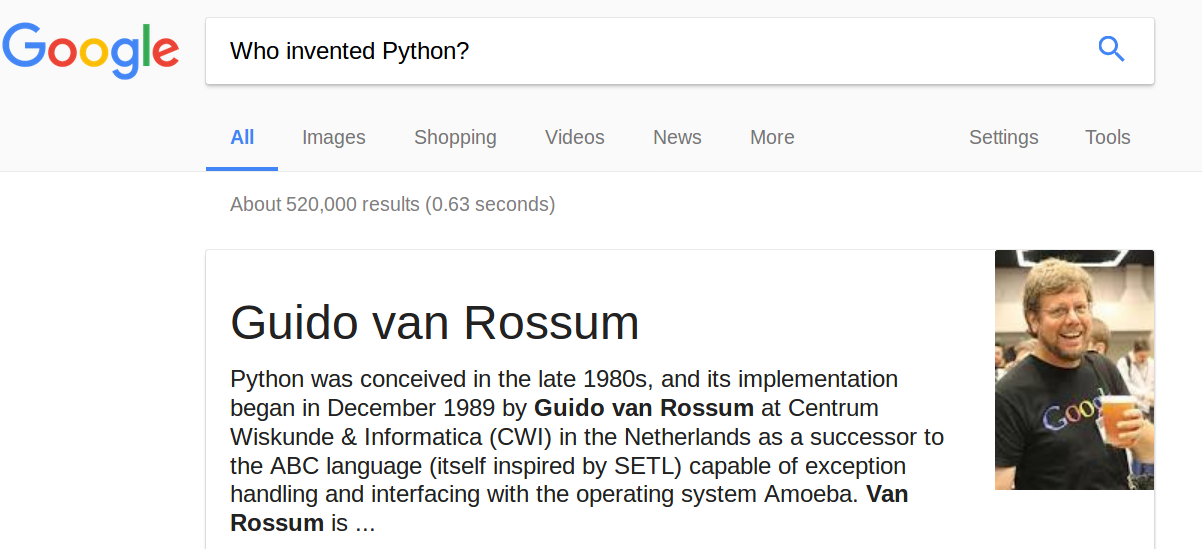
\includegraphics[width=1\linewidth]{image2/Chapitre1/guido_google.png}
	\end{minipage}
	\column{0.5\textwidth}
	\begin{minipage}[c][0.5\textheight][c]{\linewidth}
	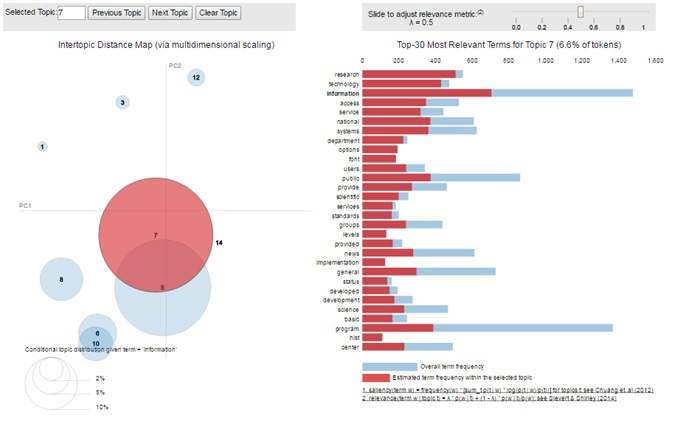
\includegraphics[width=1\linewidth]{image2/Chapitre1/lda_2d.jpg}
	\end{minipage}
	\end{columns}
	\vspace{\textheight}
\end{frame}

\begin{frame}{How do we extract meaning from text?}
%\vspace{1cm}

\begin{itemize}
\item[] {{We use \textbf{Natural Language Processing} (NLP), a field of computer science interested in making computers comprehend text and obtain useful information from it}}
\end{itemize}
\begin{figure}
\centering
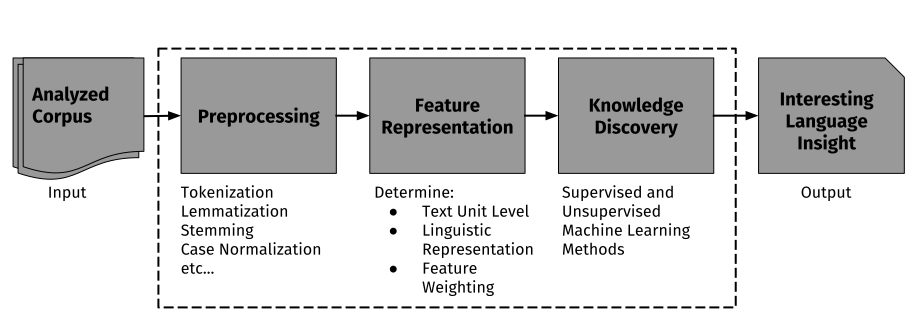
\includegraphics[width=1\linewidth]{image2/Chapitre1/nlp_flow}
\end{figure}
\vspace{\textheight}
\end{frame}

	
\begin{frame}
\frametitle{Feature Representation and Knowledge Discovery}
%\vspace{1cm}


\begin{columns}
	\column{0.5\textwidth}
	\begin{itemize}
		\item[] How do we represent text for the machine to understand? 
	\end{itemize}
	\begin{minipage}[c][0.5\textheight][c]{\linewidth}
		\centering
		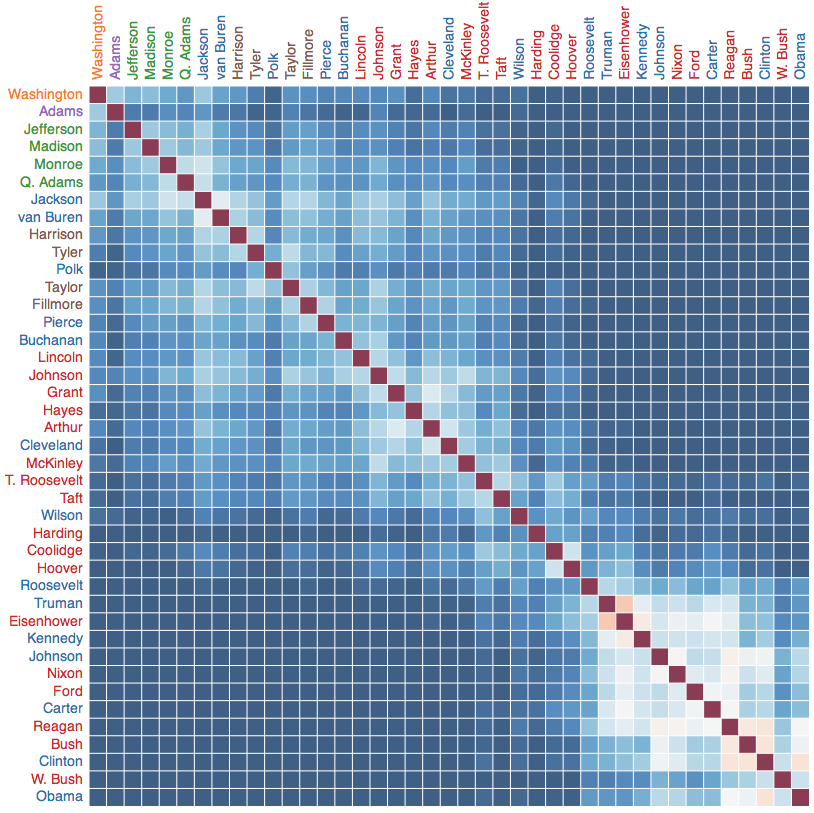
\includegraphics[width=.7\linewidth]{image2/Chapitre1/matrix.png}
	\end{minipage}
	\begin{itemize}
		\item[] Dealing with \textcolor{orangeEric}{data sparsity}
		\item[] Leveraging \textcolor{orangeEric}{heterogeneity}
	\end{itemize}	
	\column{0.5\textwidth}
	\begin{itemize}
		\item[] What techniques do we use to discover meaning from text?
	\end{itemize}
	
	\begin{minipage}[c][0.5\textheight][c]{\linewidth}
		\centering
		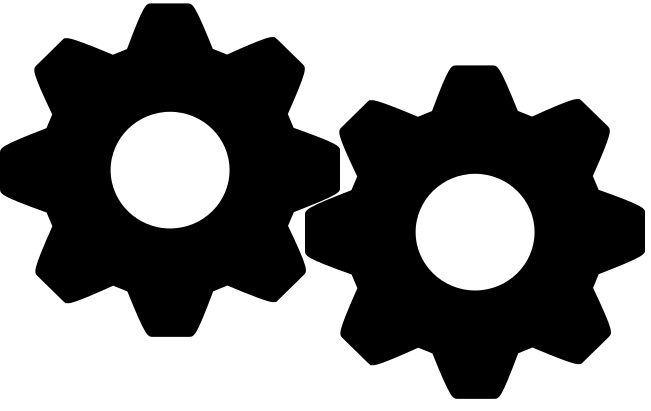
\includegraphics[width=.8\linewidth]{image2/Chapitre1/kdisc.png}

	\begin{itemize}
		\item[] Finding \textcolor{orangeEric}{semantic communities}
	\end{itemize}	
	\end{minipage}	
\end{columns}

\vspace{\textheight}

\end{frame}
%\subsection{Challenges and Contributions}

\begin{frame}{Representing Text}
%So for example, in this text, I can get features that describe its properties. They may be lexical (needing only the information of the words surrounding each word), syntactical (exaplin syntactic vs dependency tree)

\begin{itemize}
	\item \textbf{Common ways to represent text}
	\begin{itemize}
		\item Lexical
		\item Syntactic
		\begin{itemize}
				\item Constituency Tree
				\item Dependency Tree
		\end{itemize}
		\item Semantic
	\end{itemize}
	\onslide<2-> \item \textbf{Example Phrase}
	\begin{itemize}
		\item[] \textit{The report contains copies of the minutes of these meetings}
	\end{itemize}
\end{itemize}

\begin{overprint}
  				
  \onslide<3>
	  \vfill
	  \centering
	  \textbf{Lexical Representation}
	  \vspace{.3cm}
	  	  
      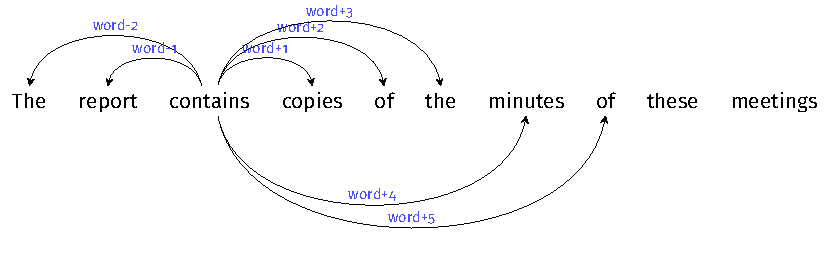
\includegraphics[width=.8\linewidth]{img/tree/lexical_tree.pdf}
	  \vfill
  \onslide<4>
	  \vfill
  	  \centering
  	  \textbf{Constituency Tree Representation}
      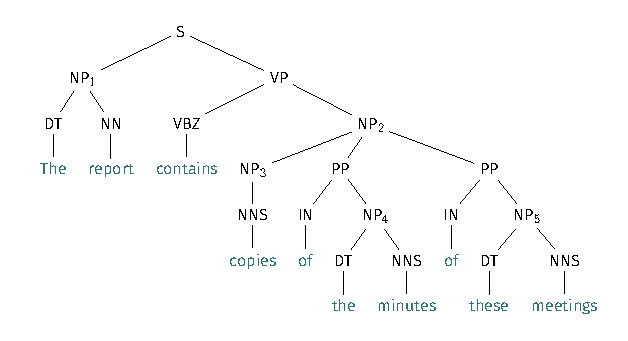
\includegraphics[width=.65\linewidth]{img/tree/tree.pdf}
      \vfill
  \onslide<5>
	  \vfill
	  \centering
   	  \textbf{Dependency Tree Representation}
   	  \vspace{.3cm}
      
      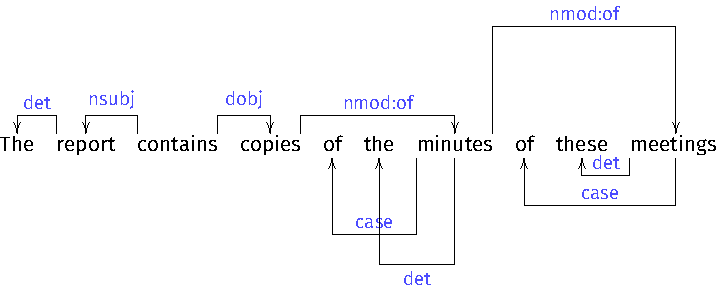
\includegraphics[width=.8\linewidth]{img/tree/dep_tree.pdf}
      \vfill
\end{overprint}
\end{frame}



%\begin{frame}{Represention Models}
%\begin{itemize}
%\item \textbf{Two classic models}
%	\begin{itemize}
%		\item Graph-based 
%		\item Matrix-based
%	\end{itemize}
%\item \textbf{Leveraging the network structure}
%	\begin{itemize}
%		\item We can find communities of similiar words according to their meaning
%	\end{itemize}
%\end{itemize}
%\begin{overprint}
%	  % on every slide (not sure if it is officially supported)
%	  \onslide<2>
%	  \centering
%	      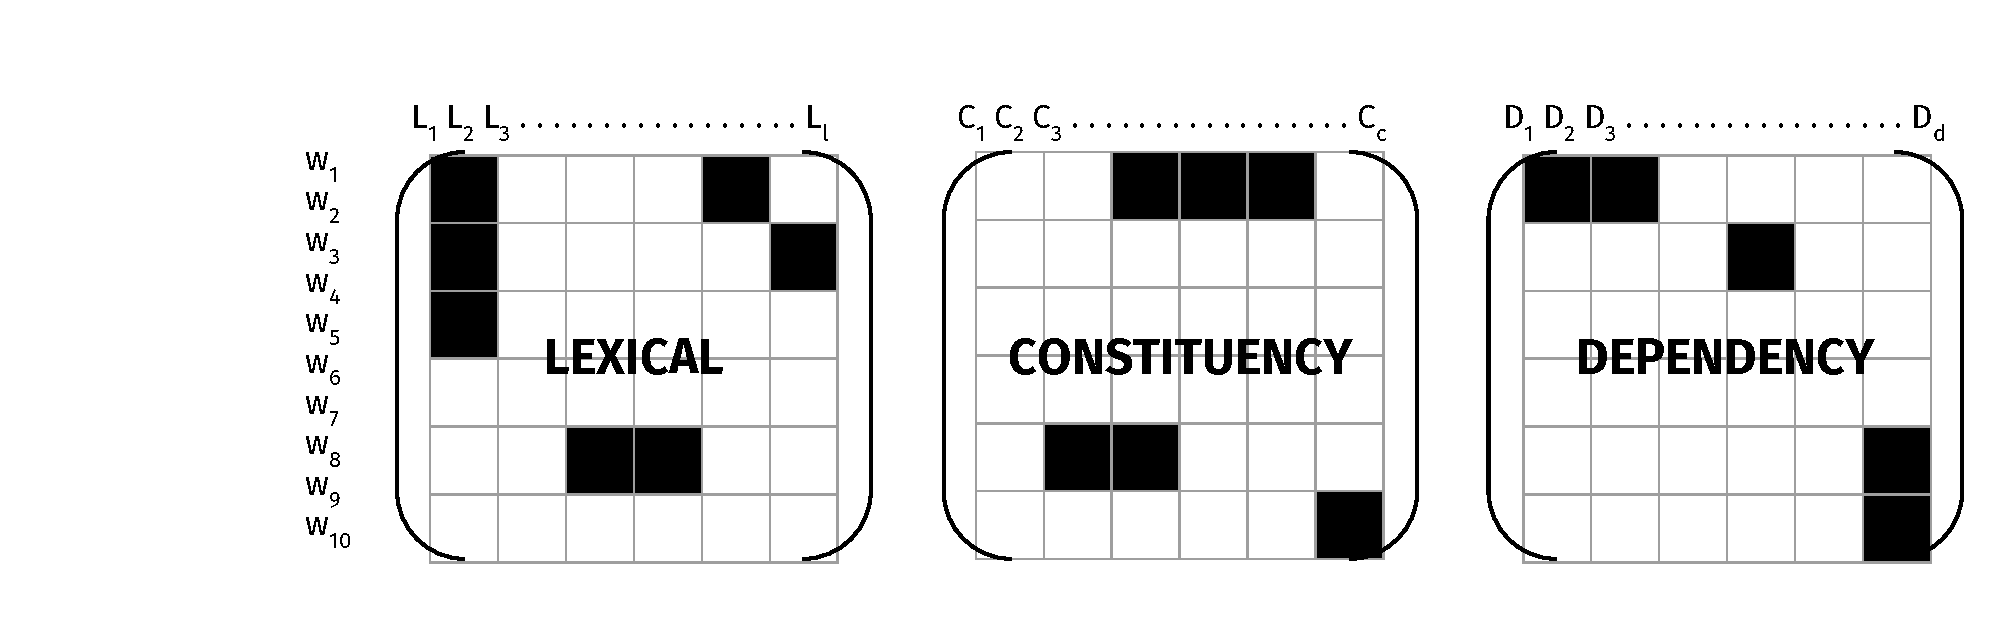
\includegraphics[width=.8\linewidth]{image2/Chapitre1/feature_types.pdf}	
%%	  \onslide<3>
%%	  \centering
%%		  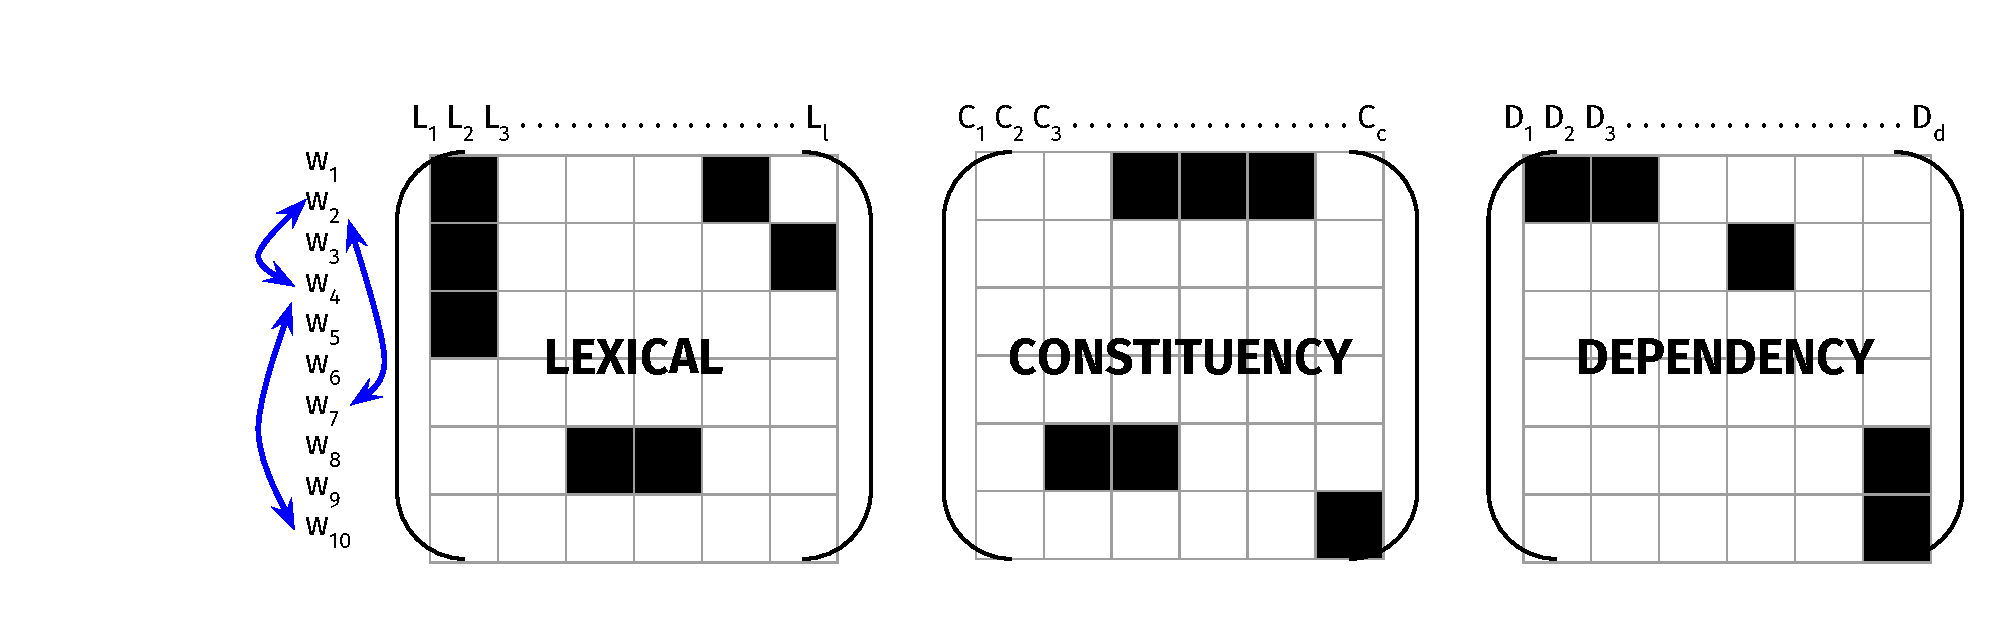
\includegraphics[width=\linewidth]{image2/Chapitre1/feature_types_communities.pdf}	  
%	  % on slide two
%\end{overprint}
%
%\end{frame}

\begin{frame}{Represention Models}
	\begin{columns}
		\column{.5\textwidth}
		\begin{minipage}[c][0.3\textheight][c]{\linewidth}
		 \centering
		 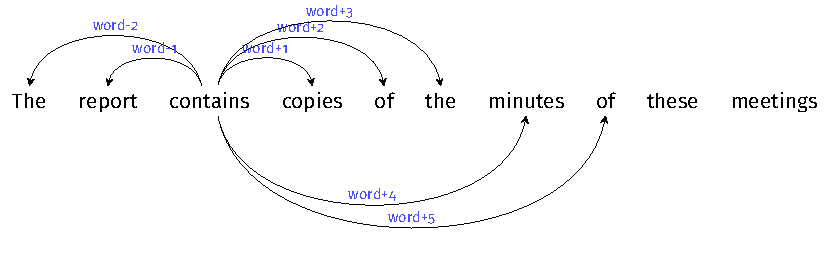
\includegraphics[width=1\linewidth]{img/tree/lexical_tree.pdf}
		\end{minipage}
		\begin{minipage}[c][0.3\textheight][c]{\linewidth}
		 \centering
		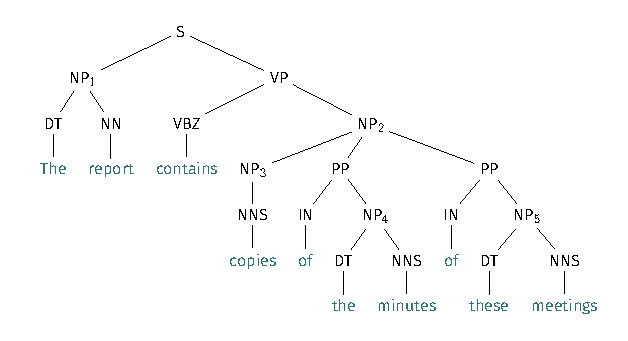
\includegraphics[width=1\linewidth]{img/tree/tree.pdf}
		\end{minipage}
		\begin{minipage}[c][0.3\textheight][c]{\linewidth}
		\centering
		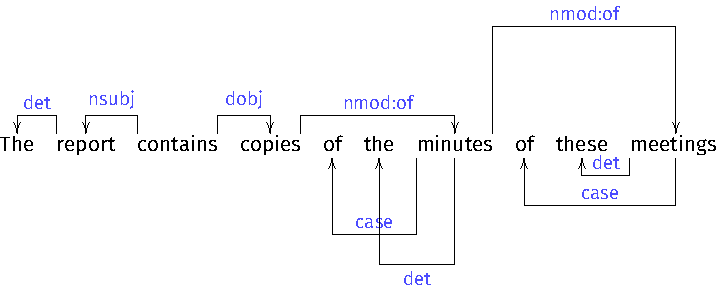
\includegraphics[width=1\linewidth]{img/tree/dep_tree.pdf}
		\end{minipage}
		\column{.5\textwidth}
		\begin{minipage}[c][0.3\textheight][c]{\linewidth}
		 \centering
		 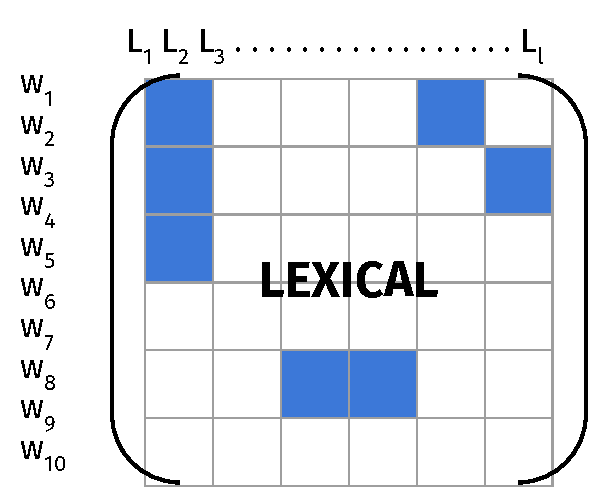
\includegraphics[width=.6\linewidth]{image2/Chapitre1/lexical.pdf}
		\end{minipage}
		\begin{minipage}[c][0.3\textheight][c]{\linewidth}
		 \centering
		 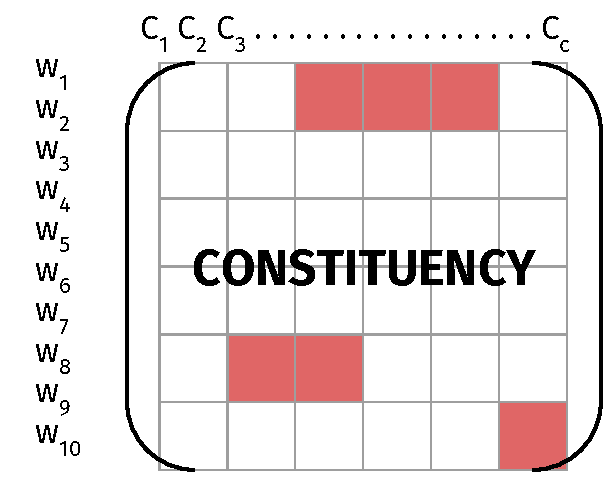
\includegraphics[width=.6\linewidth]{image2/Chapitre1/syn_1.pdf}
		\end{minipage}
		\begin{minipage}[c][0.3\textheight][c]{\linewidth}
		\centering
		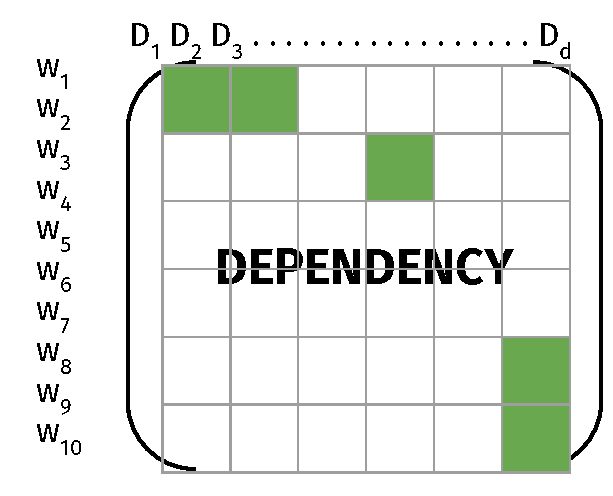
\includegraphics[width=.6\linewidth]{image2/Chapitre1/dep_1.pdf}
		\end{minipage}	
	\end{columns}
\end{frame}


\begin{frame}{Main Challenges and Contributions}
\vspace{1cm}
	\begin{enumerate}
		\item<1-> What type of model can we employ to represent a corpus  \textcolor{orangeEric}{using heterogeneous features}?
		\begin{itemize}
		\item<1-> \textit{Hypergraph model to  \textcolor{greenEric}{hold different types of  linguistic information}}
		\end{itemize}
		
		\item<2-> How can we combine these features while  \textcolor{orangeEric}{dealing with feature sparsity}?
		\begin{itemize}
		\item<2-> \textit{Multimedia fusion techniques to \textcolor{greenEric}{combine and densify} representation spaces}	    	 
		\end{itemize}
		\item<3-> How can we \textcolor{orangeEric}{find communities} existing within the language networks?
		\begin{itemize}
		\item<3-> \textit{An alternative network-based algorithm to \textcolor{greenEric}{discover semantically related words} within a text}
		\end{itemize}
		
	\end{enumerate}
 \vspace{\textheight}
\end{frame}


\begin{frame}{Work Overview}
\begin{center}
\vfill
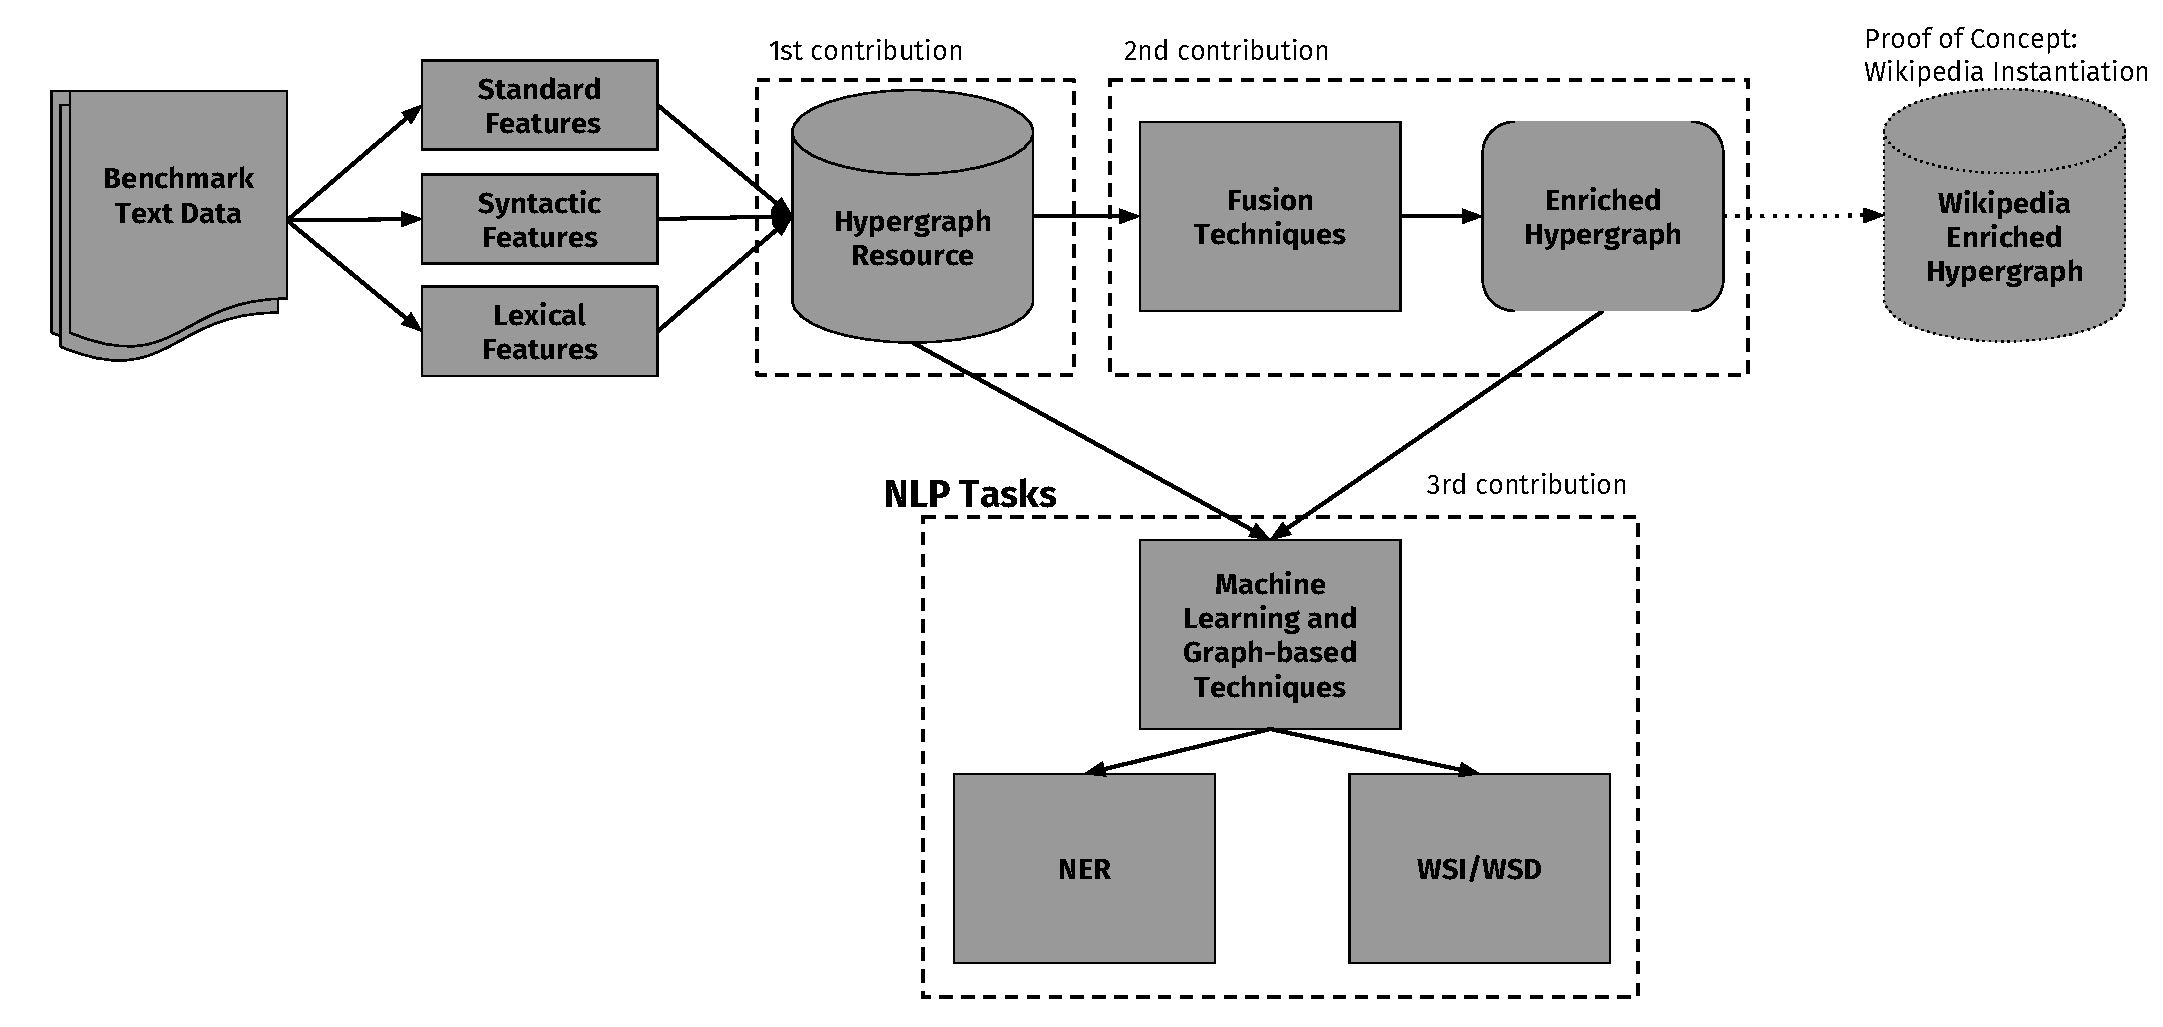
\includegraphics[width=1.04\linewidth]{image2/Chapitre1/main_diag_presi.pdf}
\end{center}
\vfill
% \vspace{\textheight}
\end{frame}

\setbeamertemplate{section page}[mytheme]

\section[Contributions in Detail]{Hypergraph Linguistic Model}
\metroset{sectionpage=none}
\section{Hypergraph Linguistic Model}
\metroset{sectionpage=simple}
%\begin{frame}{Work Overview}
%%\large  \textbf{Approach Overview} \hfill
%\begin{center}
%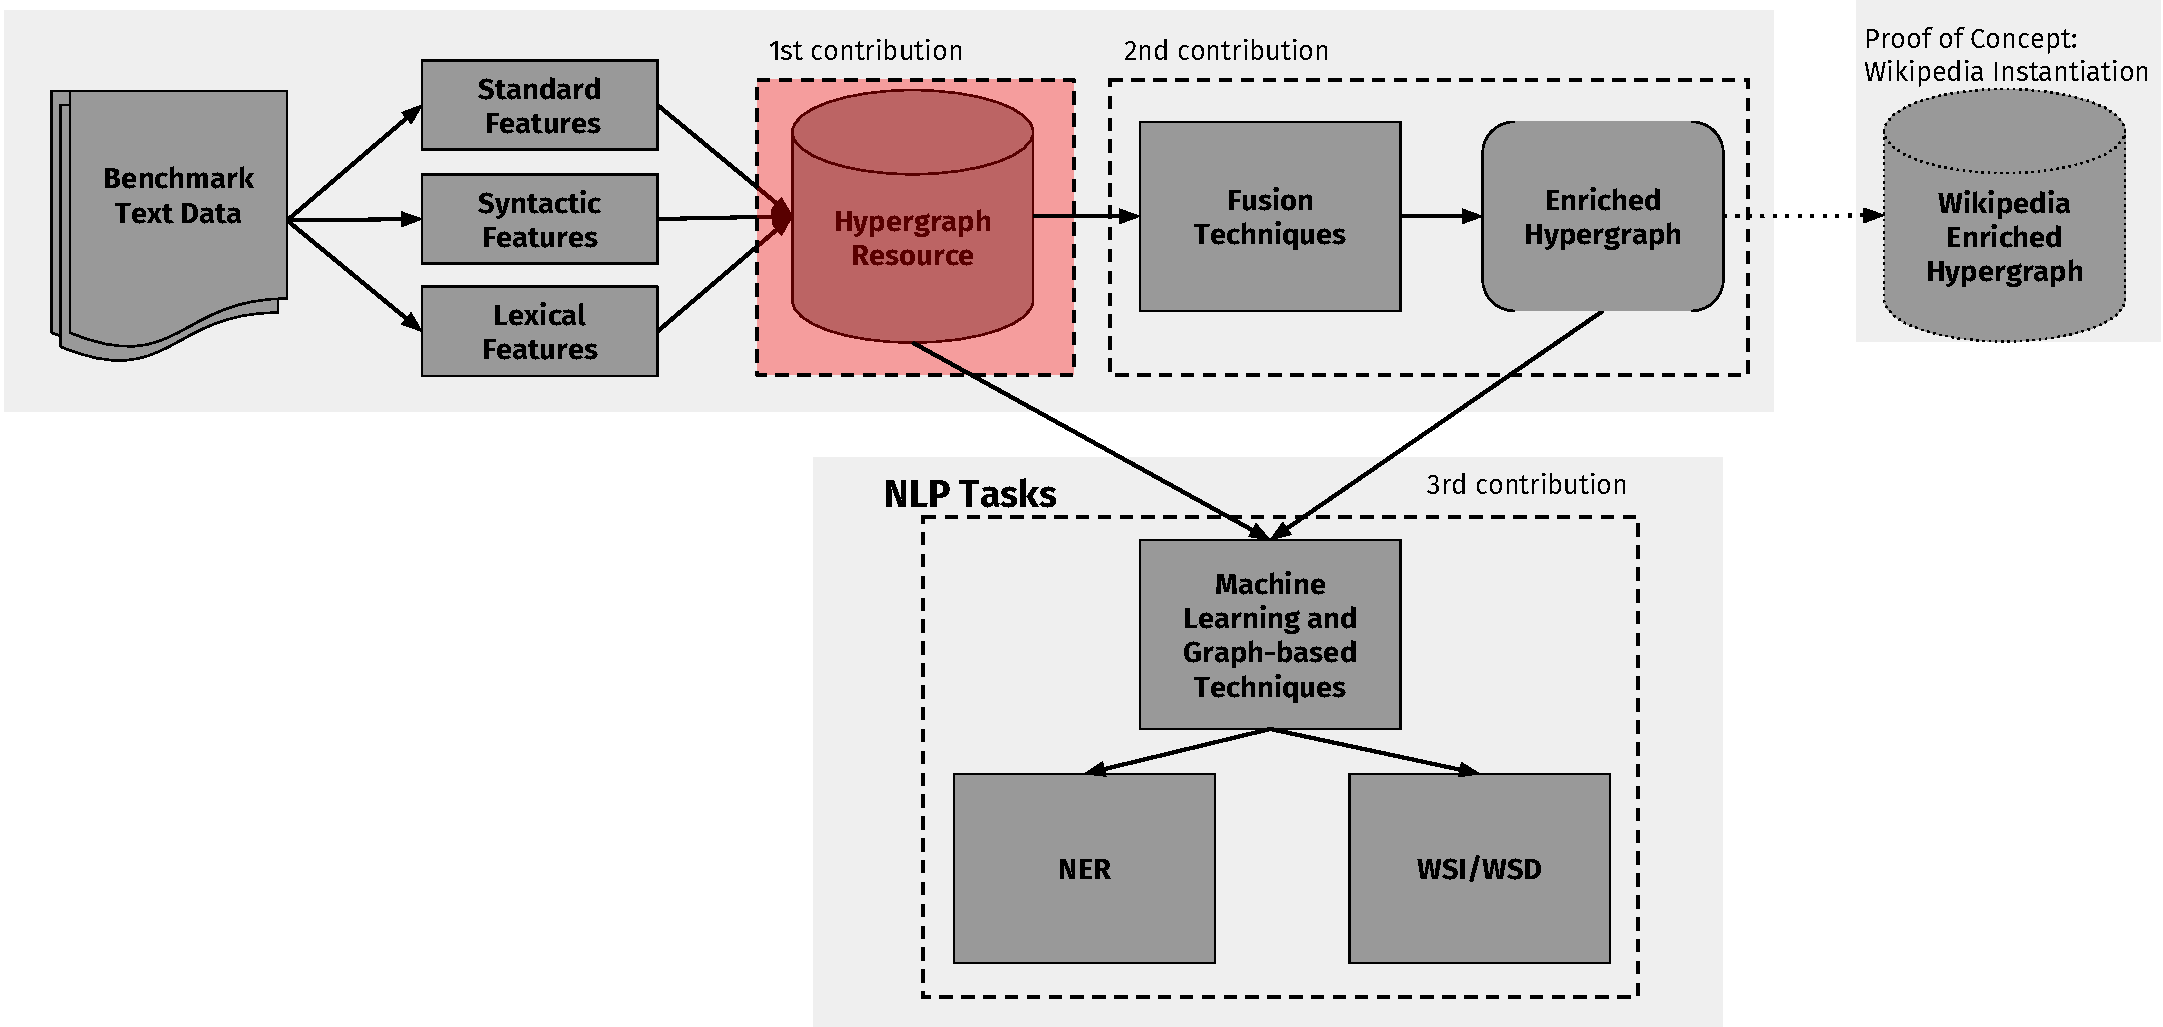
\includegraphics[width=1.04\linewidth]{image2/Chapitre3/main_diag_contr1.pdf}
%\end{center}
%
% \vspace{\textheight}
%\end{frame} 


\begin{frame}{Introduction}


\begin{itemize}
	\item<1-> \textbf{Leveraging contexts}
	\begin{itemize}
	\item<1-> We extract linguistic information from words based on the \textcolor{orangeEric}{distributional hypothesis} (a word is defined by its surroundings)
	\item<1-> These surroundings are defined as contexts
	\item<1-> Contexts are formed by the interactions a word participates in. These interactions can be lexical or syntactical or other types.

	\end{itemize}
	\item<2-> \textbf{We use network models to represent contexts} 
		\begin{itemize}

		\item<2-> Graphs structures can give us a clearer view into the relations of words within a text 	
		\item<2-> Allow us to apply methods from graph theory
		\item<2-> Ultimately graphs are transformed to a vectorial representation through the adjacency/incidence matrices
		
		\end{itemize}
		
\end{itemize}
\vspace{\textheight}
\end{frame}




\begin{frame}{Classic Language Networks}
%What is the state of the art ? How is text is represented by means of networks?
% Three main types
%todo Add here the networks by choudhury et al venus stuff

\begin{itemize}
\item[] \large \textbf{Example phrase}
\item[] \textit{The report contains copies of the minutes of these meetings} 
\end{itemize}

\begin{overprint}
  % on every slide (not sure if it is officially supported)
  \onslide<2>
	  \centering
	  
	  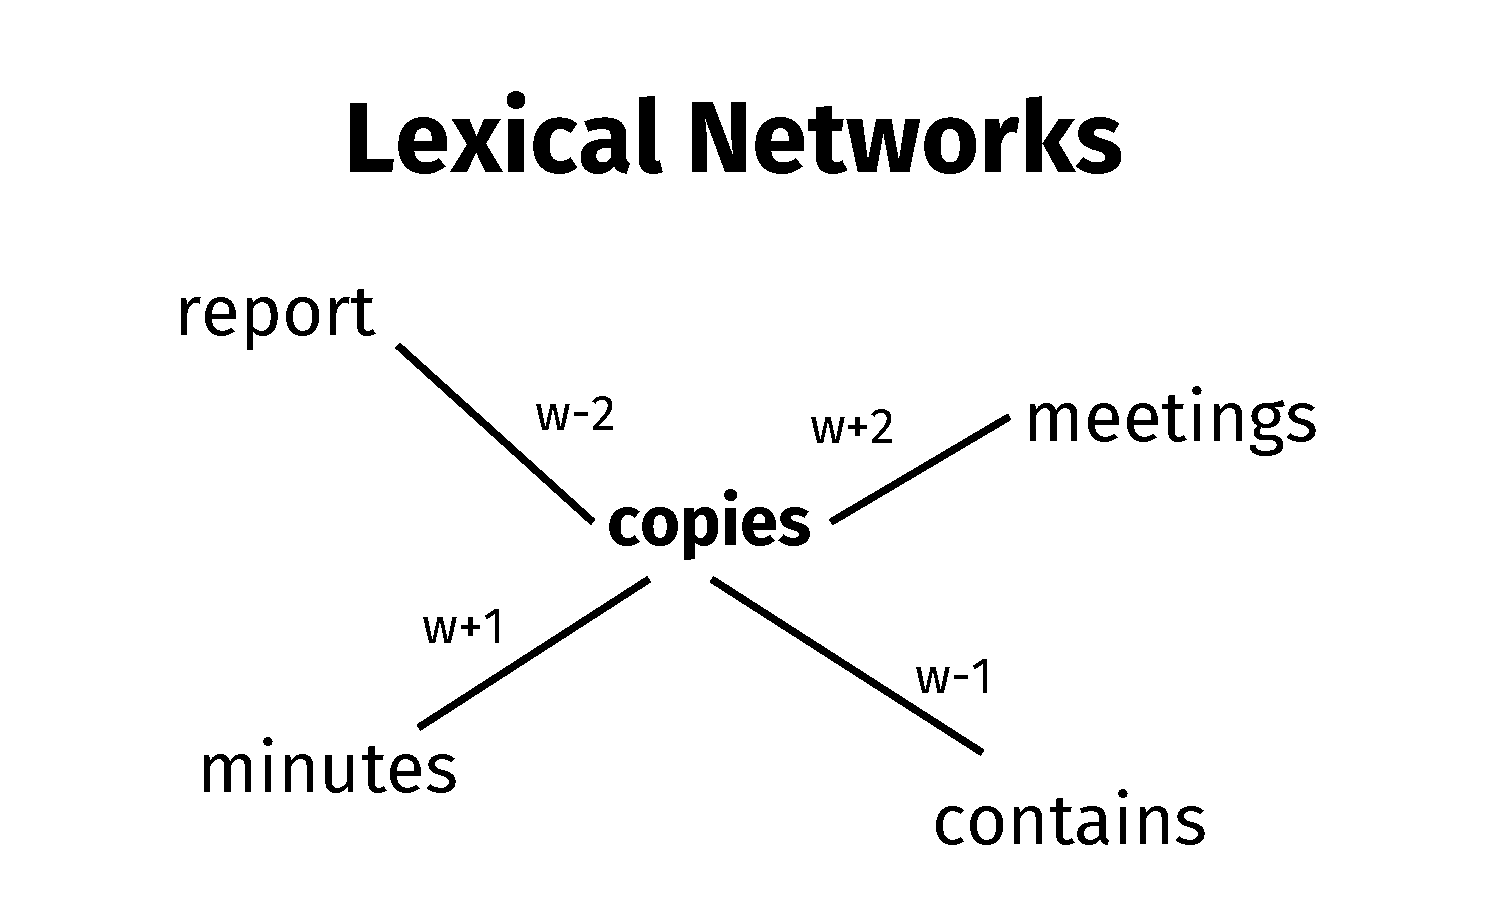
\includegraphics[width=.6\linewidth]{image2/Chapitre2/lexi_network_ex.pdf}
%	  \\ \cite{2008.Klapaftis.WSIUsingCollocations}
  \onslide<3>
	  \centering
  	  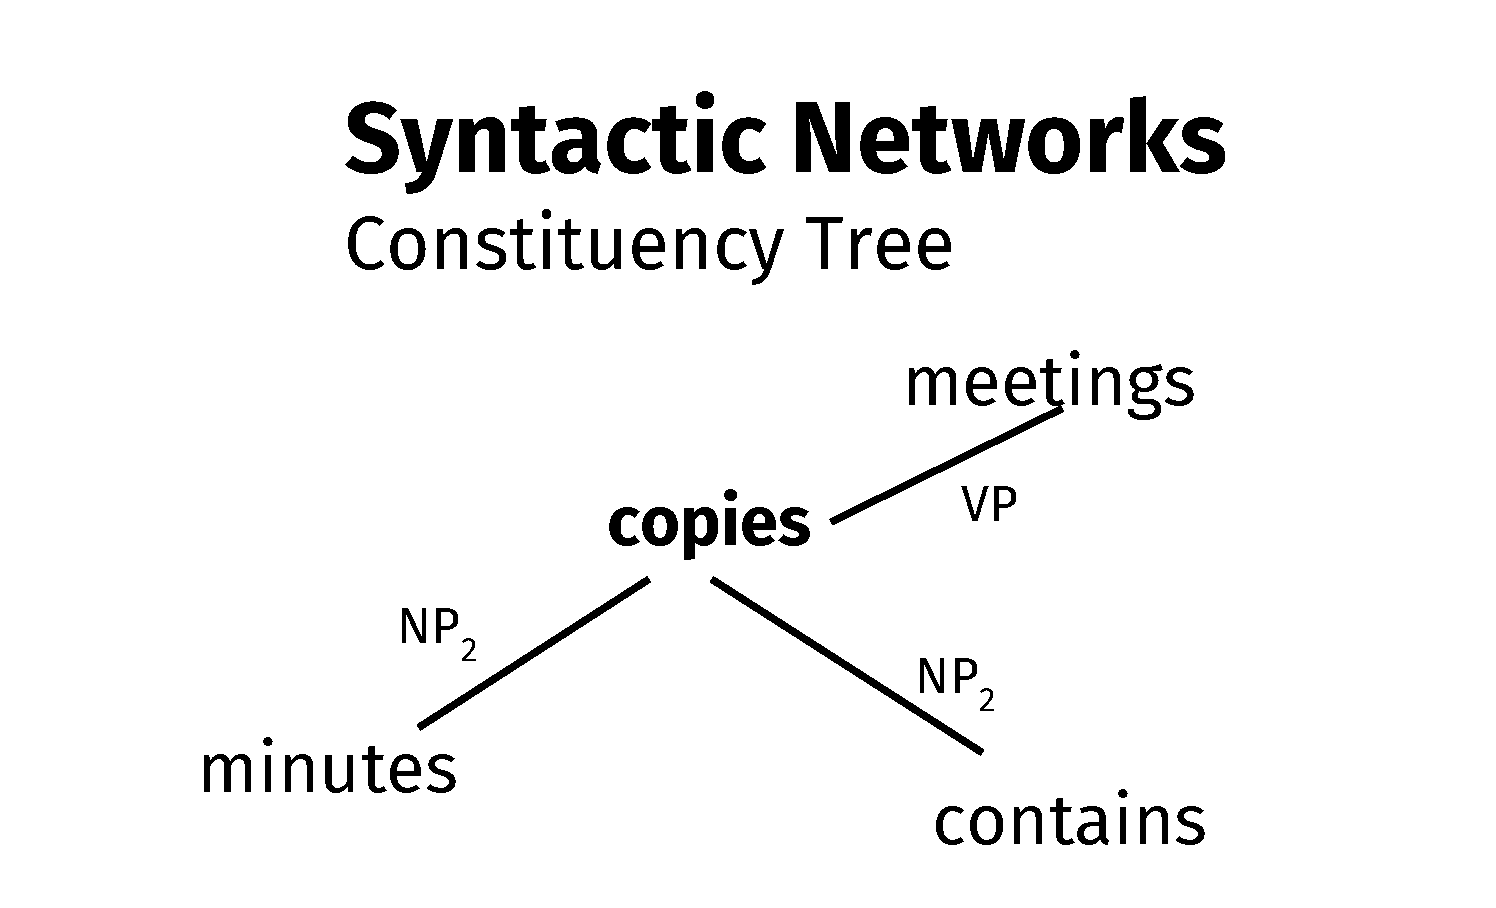
\includegraphics[width=.6\linewidth]{image2/Chapitre2/consti_network_ex.pdf}   
  \onslide<4>
	  \centering
	  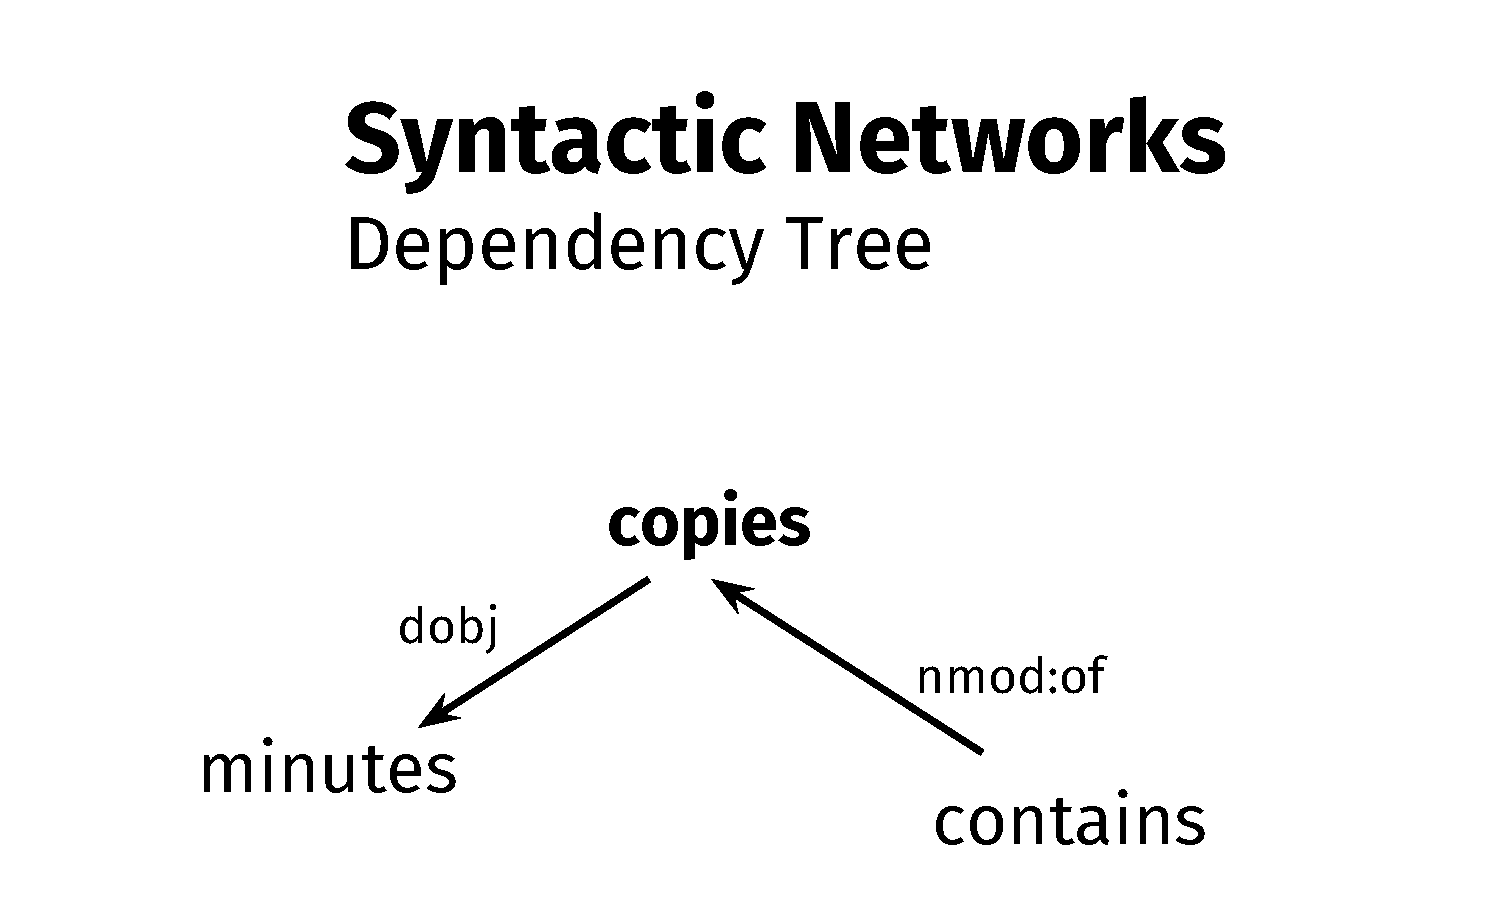
\includegraphics[width=.6\linewidth]{image2/Chapitre2/deps_network_ex.pdf} 
%  \onslide<5>
%	  \centering
%	  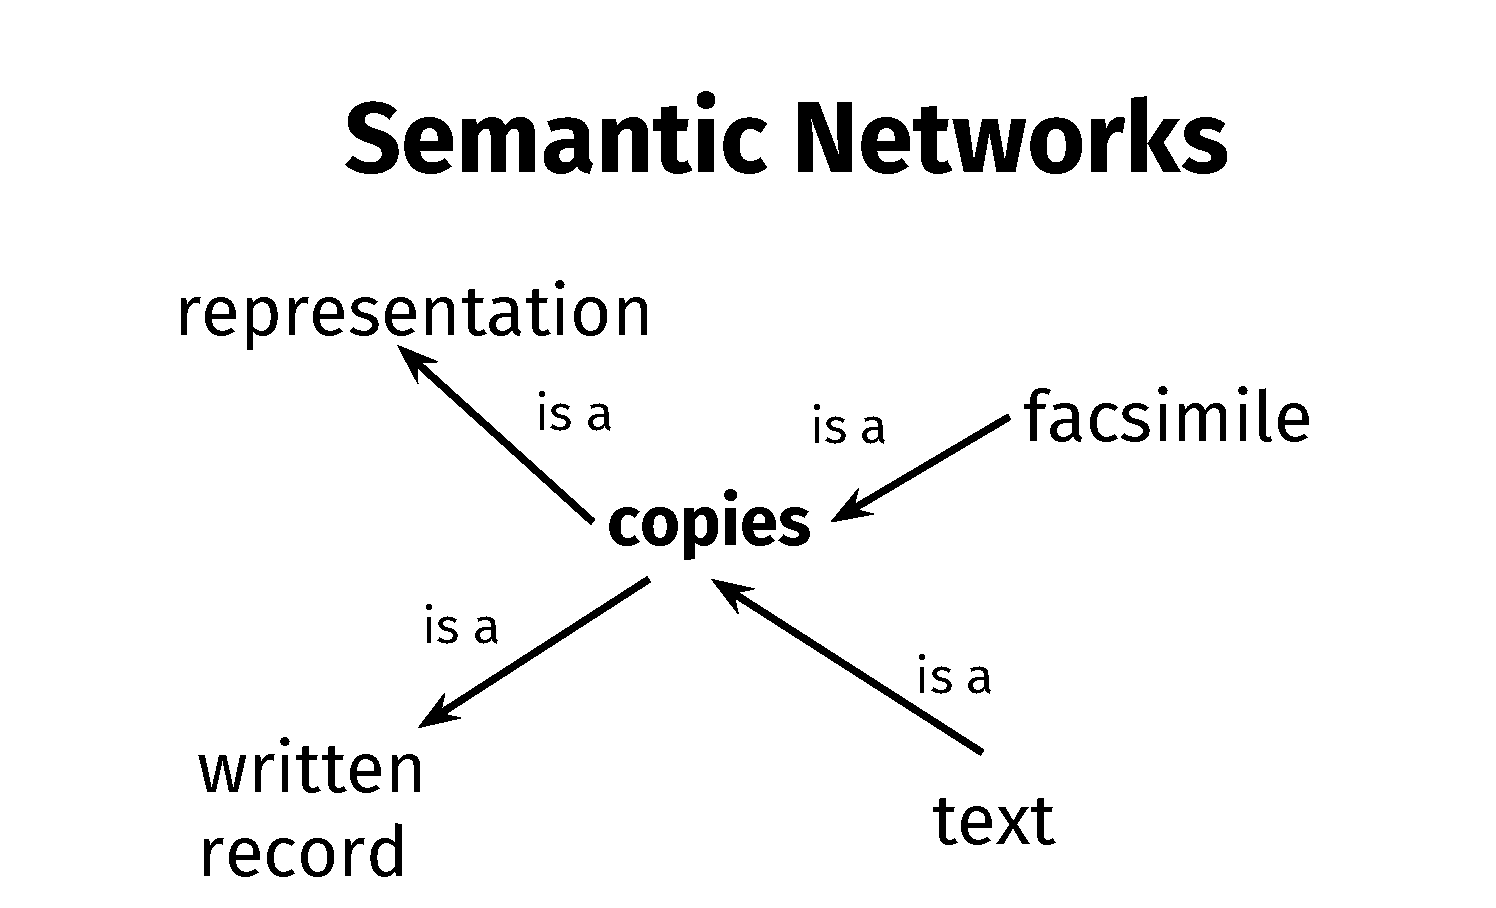
\includegraphics[width=.7\linewidth]{image2/Chapitre2/sem_network_ex.pdf}   

  % on slide three
  % etc.
\end{overprint}


\end{frame}


\begin{frame}{Limitations and Proposition}
\begin{itemize}
\item<1-> \large \textbf{Limitations of existing representations}
	\begin{itemize}
	\item<1-> Language networks generally employ a single type of textual information
	\item<1-> The edges of the network relate maximum two words at each time
	\end{itemize}
\item<2-> \large \textbf{Proposition}
	\begin{itemize}
	\item<2-> Use a hypergraph model to link together the different types of networks
	\item<2-> This allows for a semantic overview at three different layers: short range, medium range, and long range at once
	\item<2-> Relating more than two words at the same time
	\end{itemize}
\end{itemize}
\vspace{\textheight}
\end{frame}

\begin{frame}{Proposed Model}
%	\begin{itemize}
%		\item Explain (grpahically/with the working exampleh) we use lexical and syntactic info and the build a fusion of them with a hypergraph.
%	\end{itemize}
	\begin{columns}
		\column{.33\textwidth}
		\begin{minipage}[c][0.4\textheight][c]{\linewidth}
			 \centering
			 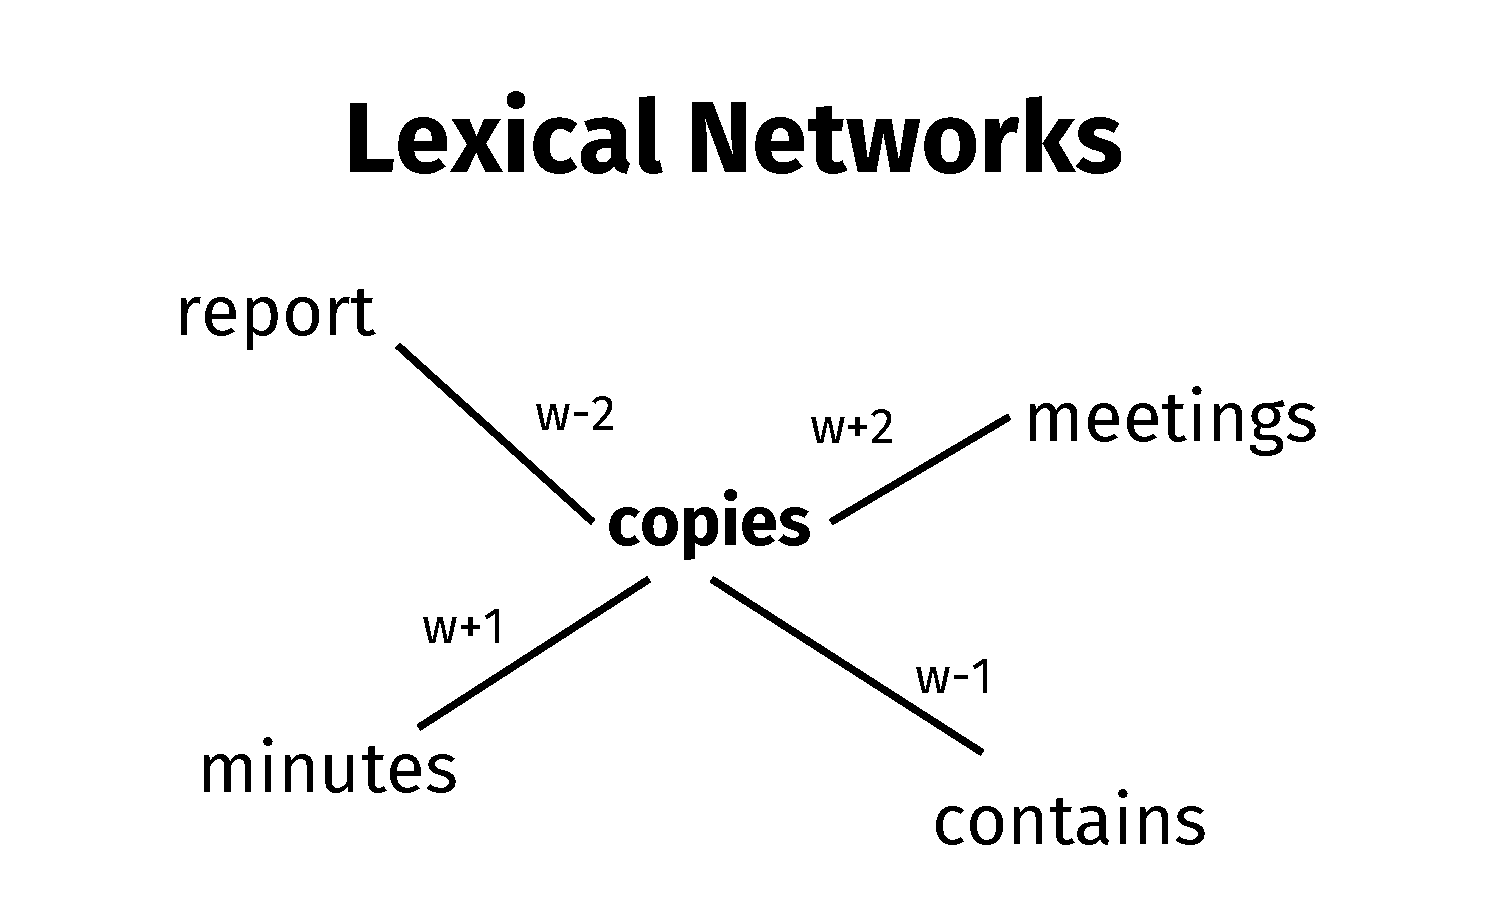
\includegraphics[width=1\linewidth]{image2/Chapitre2/lexi_network_ex.pdf}
		\end{minipage}
		\column{.33\textwidth}
		\begin{minipage}[c][0.4\textheight][c]{\linewidth}
			 \centering
			 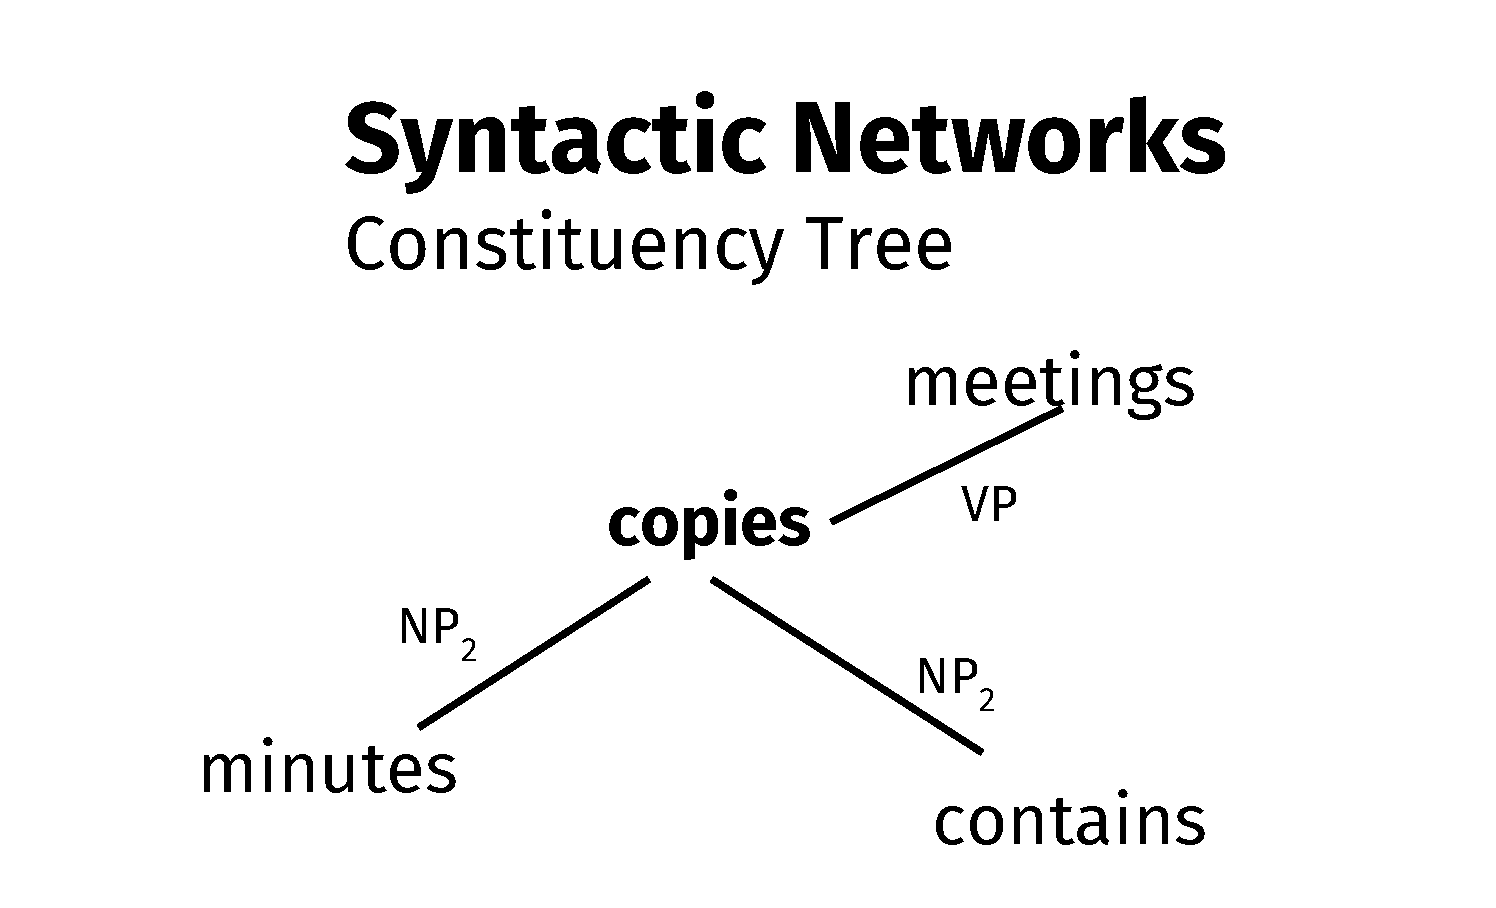
\includegraphics[width=1\linewidth]{image2/Chapitre2/consti_network_ex.pdf}
		\end{minipage}		
		\column{.33\textwidth}
		\begin{minipage}[c][0.4\textheight][c]{\linewidth}
			 \centering
				 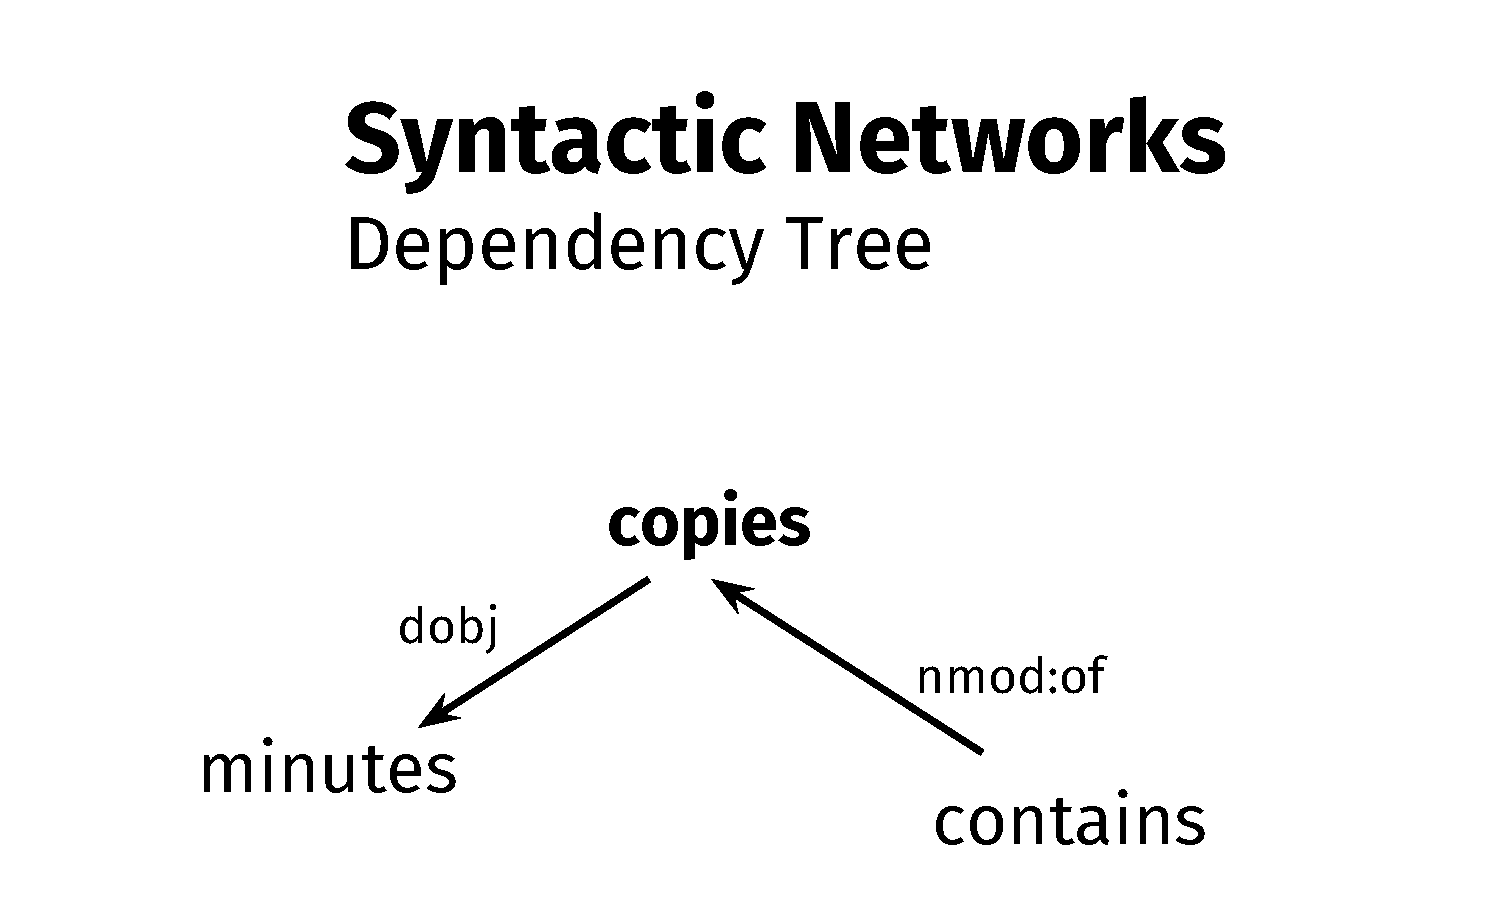
\includegraphics[width=1\linewidth]{image2/Chapitre2/deps_network_ex.pdf}
		\end{minipage}
	\end{columns}
	

	
	\begin{overprint}
	\onslide<2>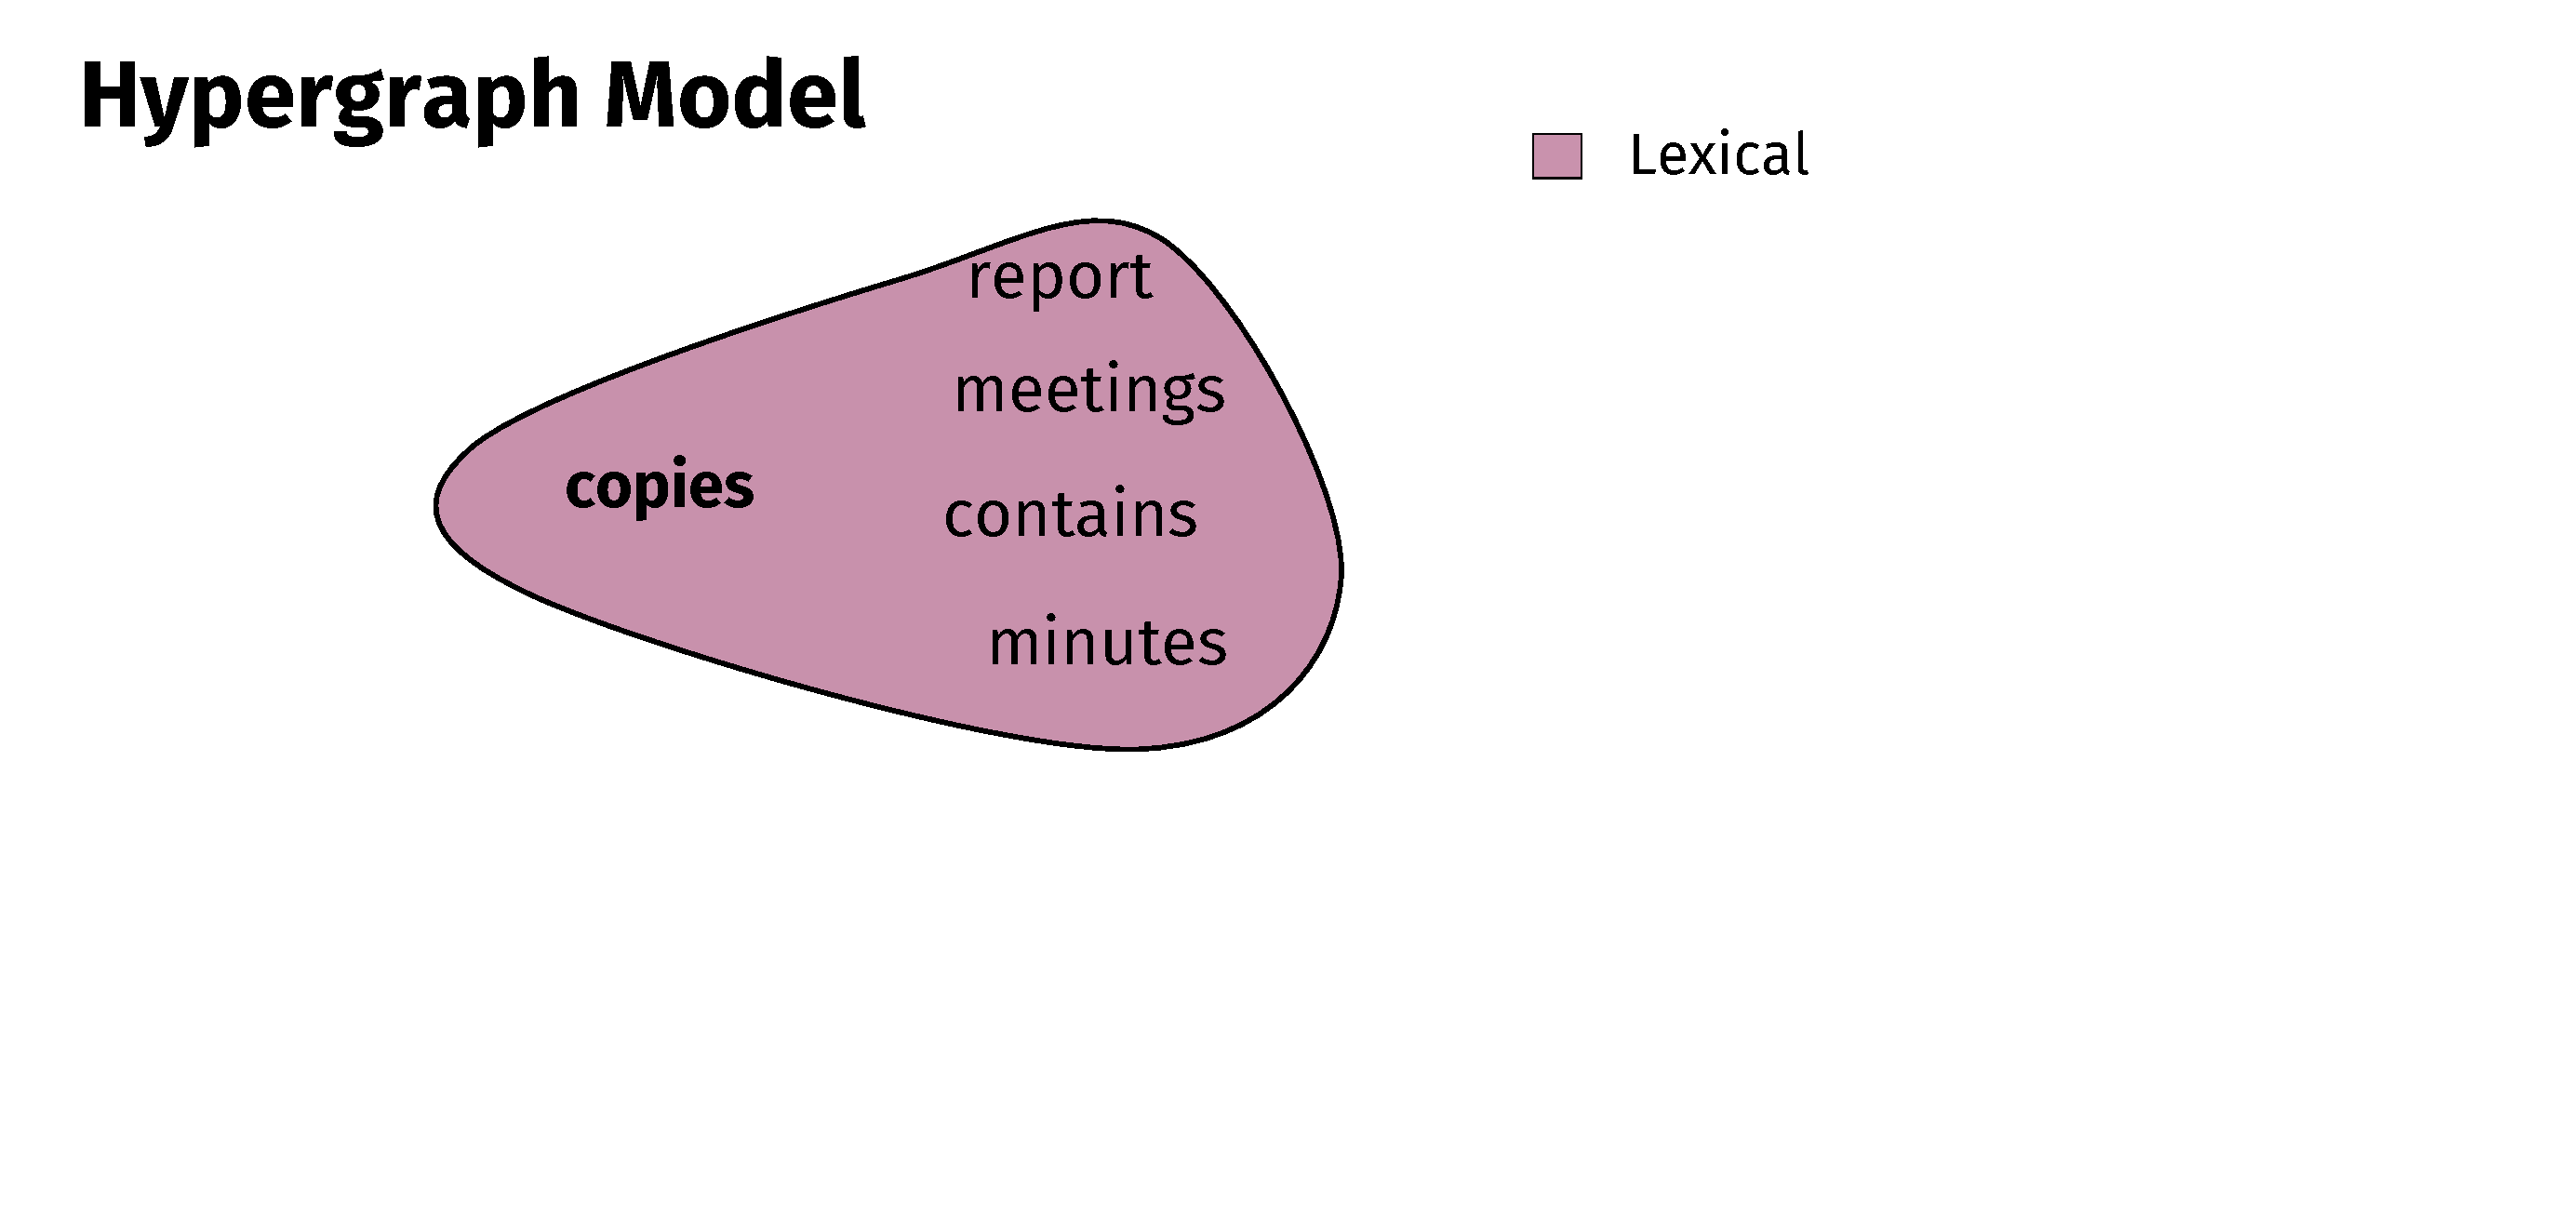
\includegraphics[width=1\linewidth]{image2/Chapitre2/hyper_network_ex_1.pdf}%lexical
	\onslide<3>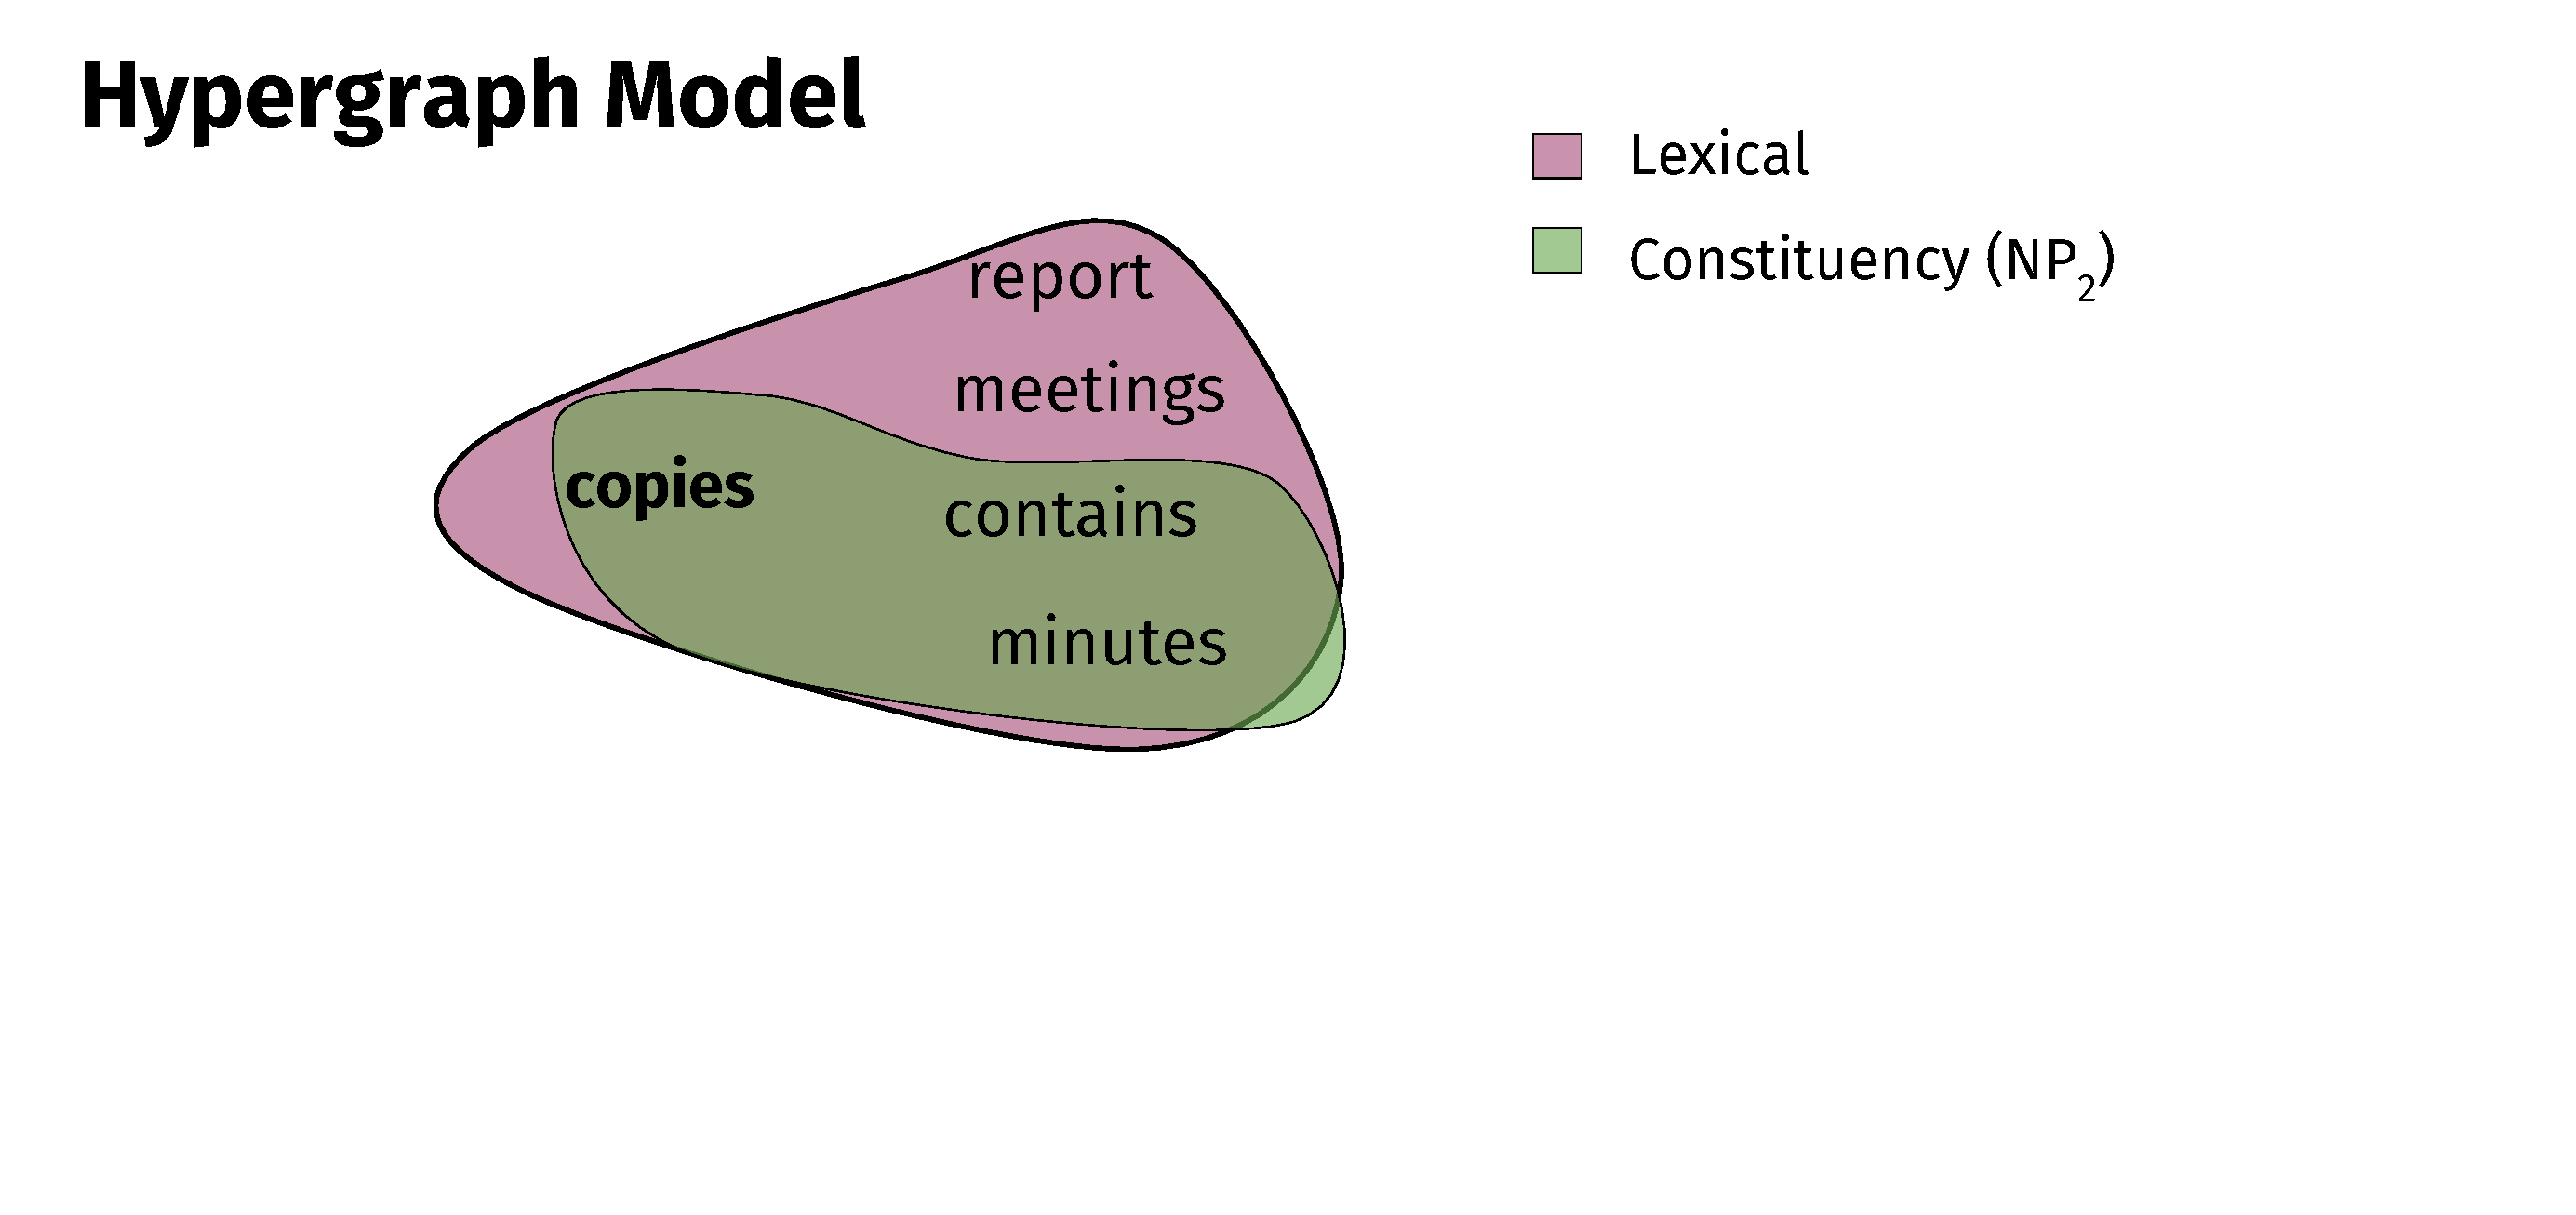
\includegraphics[width=1\linewidth]{image2/Chapitre2/hyper_network_ex_2.pdf}%constit
	\onslide<4>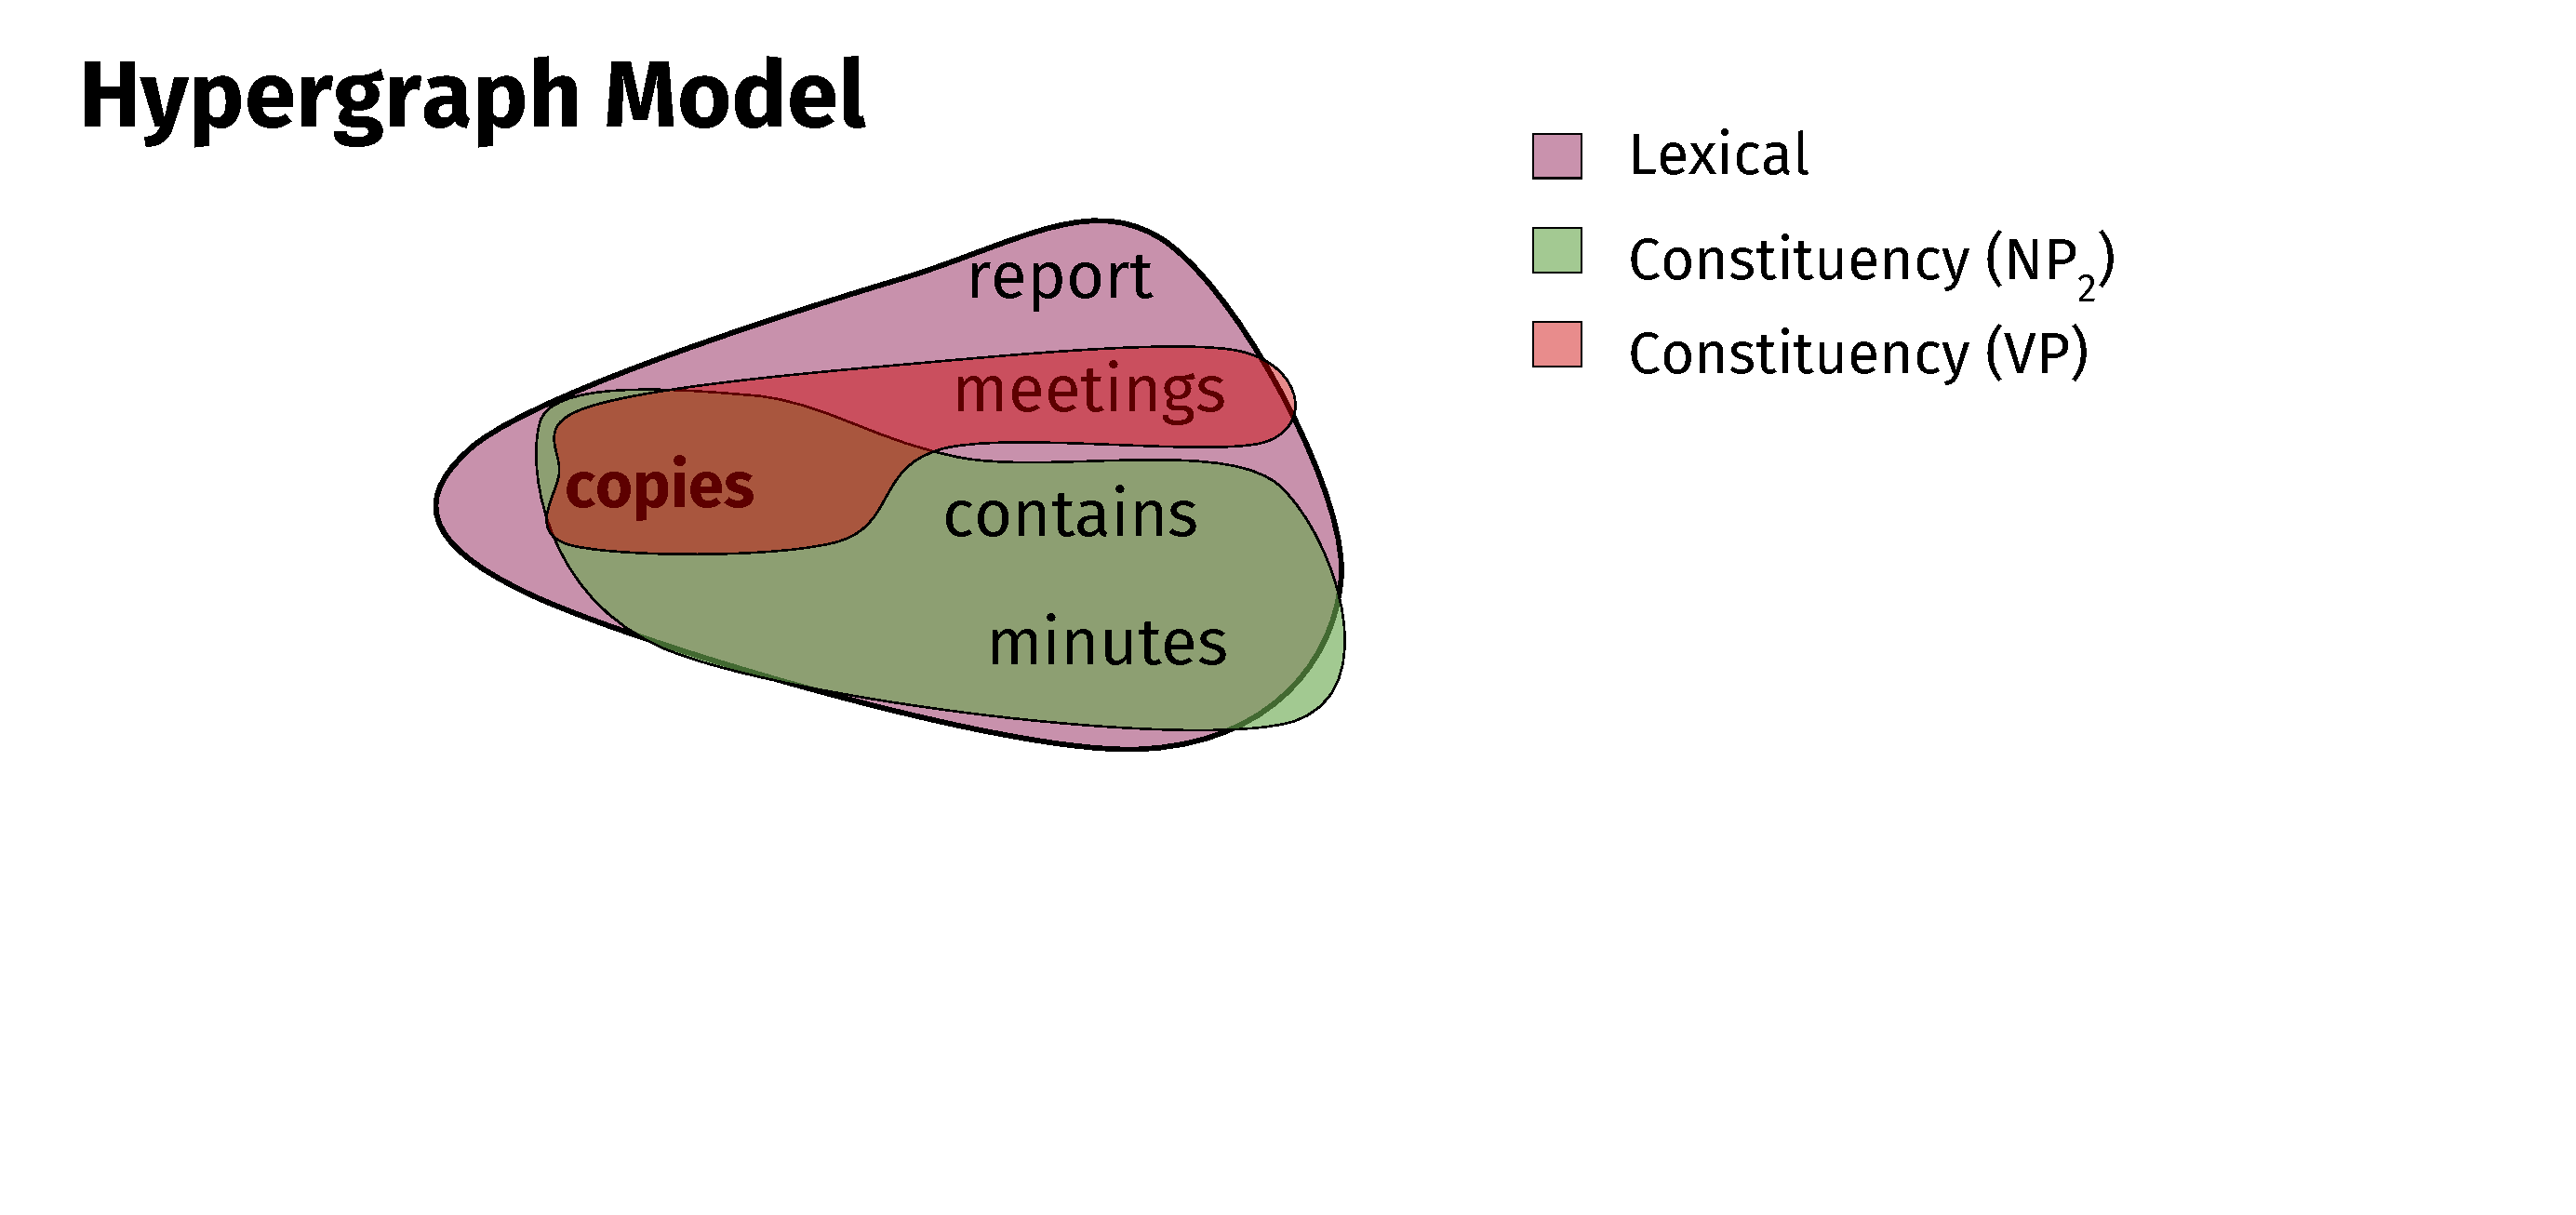
\includegraphics[width=1\linewidth]{image2/Chapitre2/hyper_network_ex_3.pdf}%constit
	\onslide<5>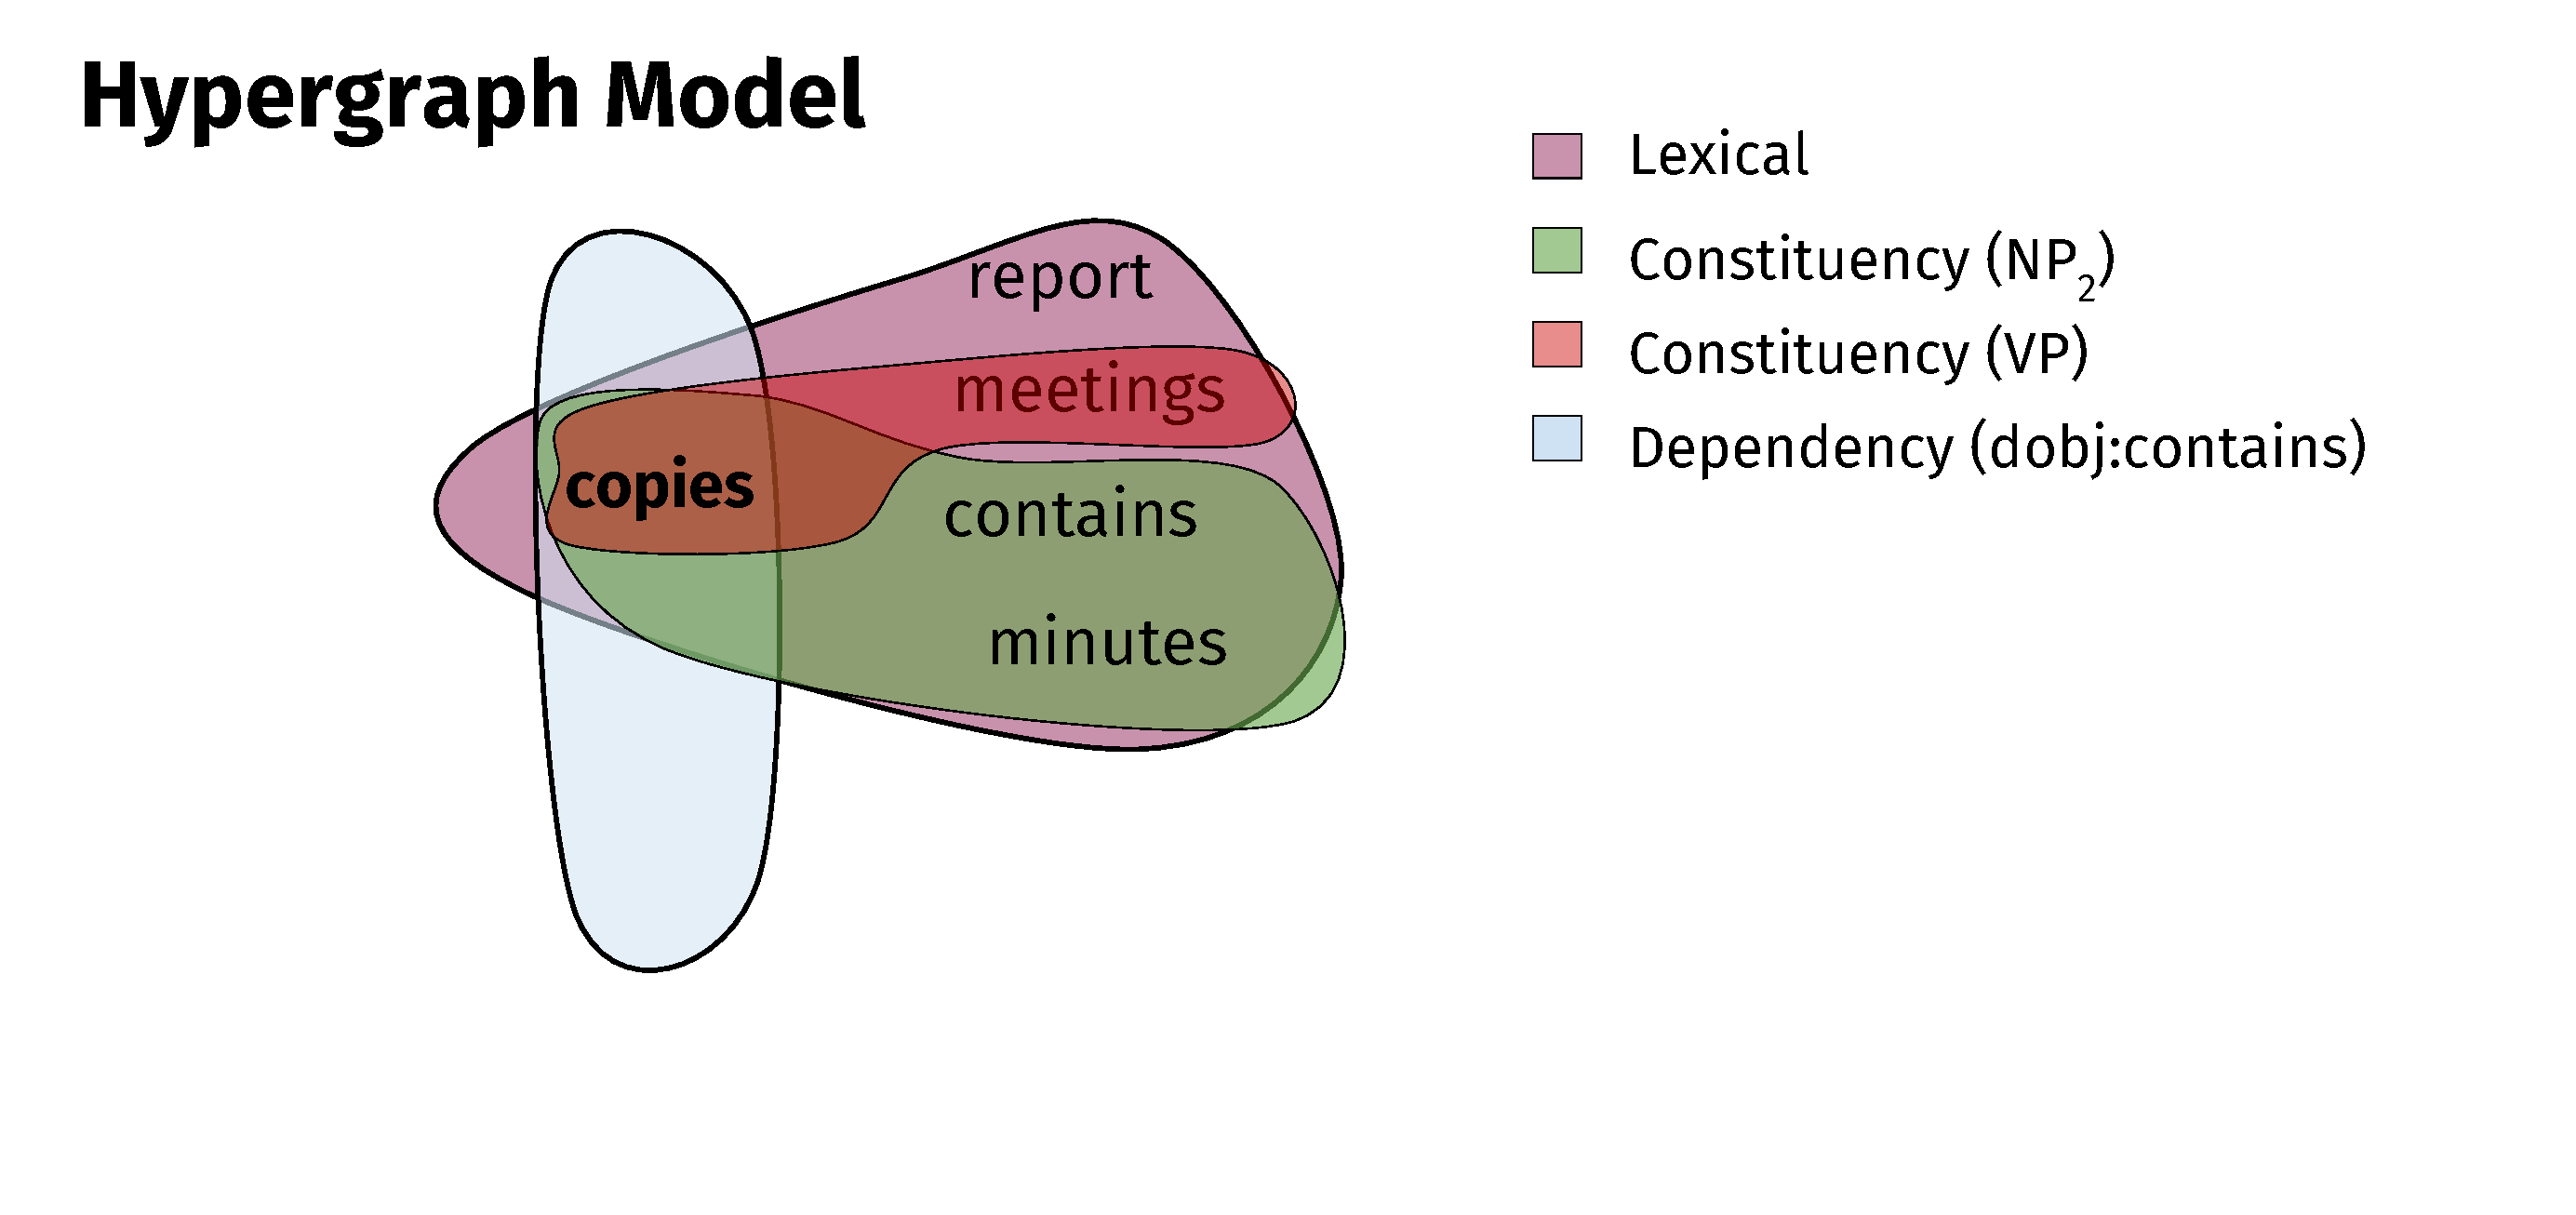
\includegraphics[width=1\linewidth]{image2/Chapitre2/hyper_network_ex_4.pdf}%dep
	\onslide<6>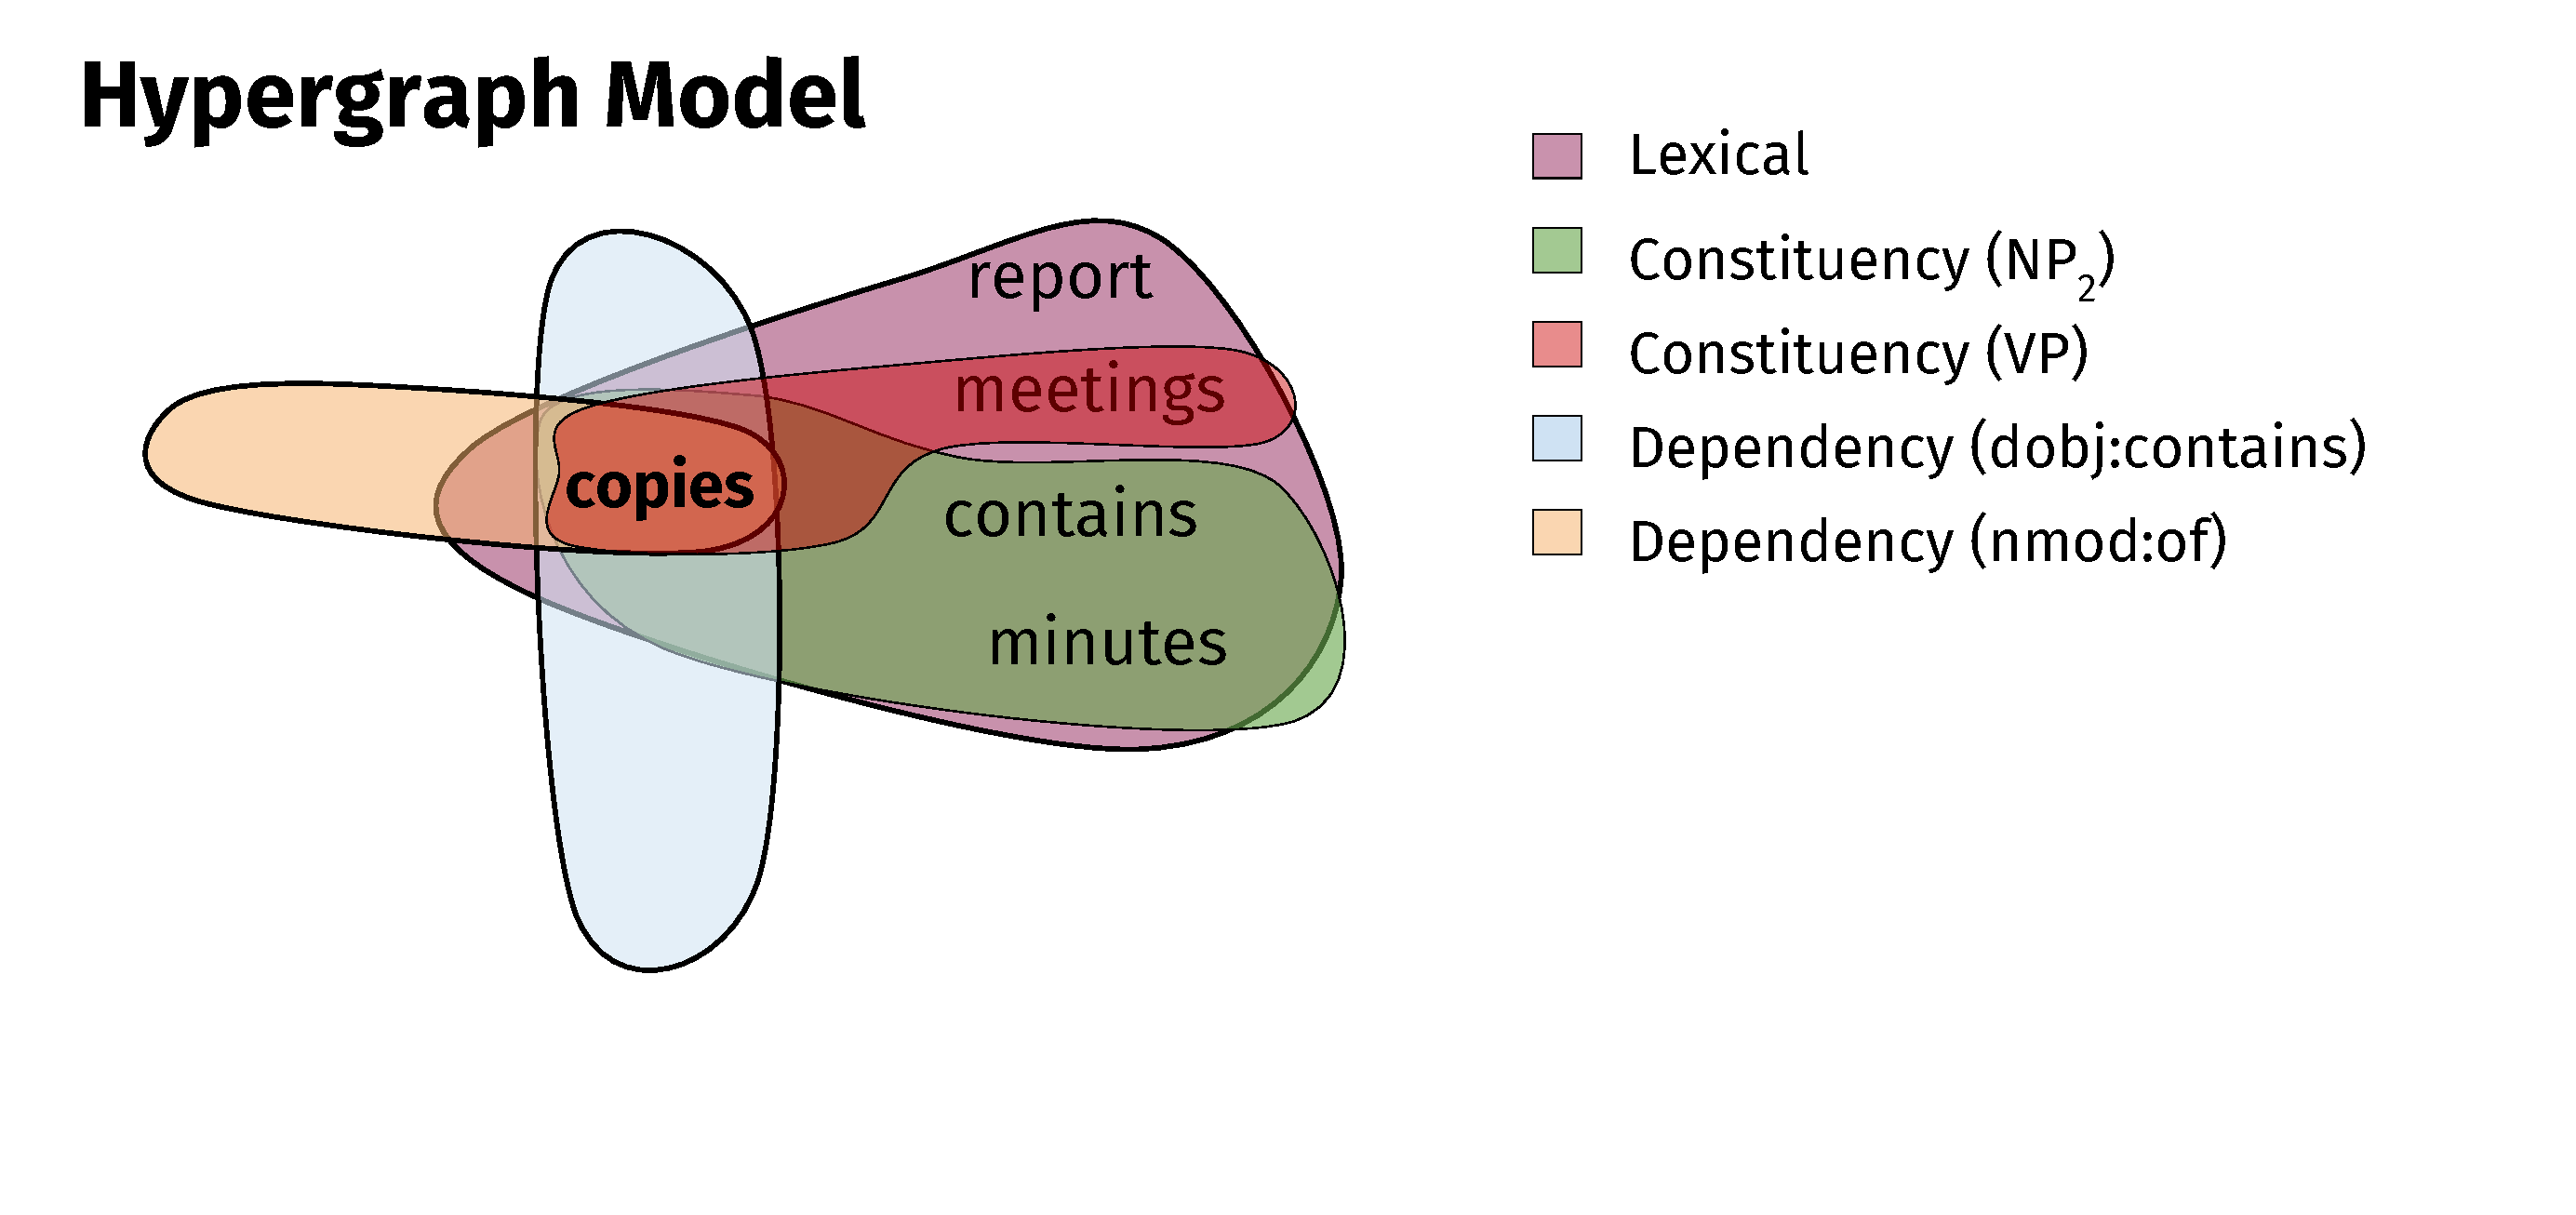
\includegraphics[width=1\linewidth]{image2/Chapitre2/hyper_network_ex_5.pdf}%dep
	\onslide<7>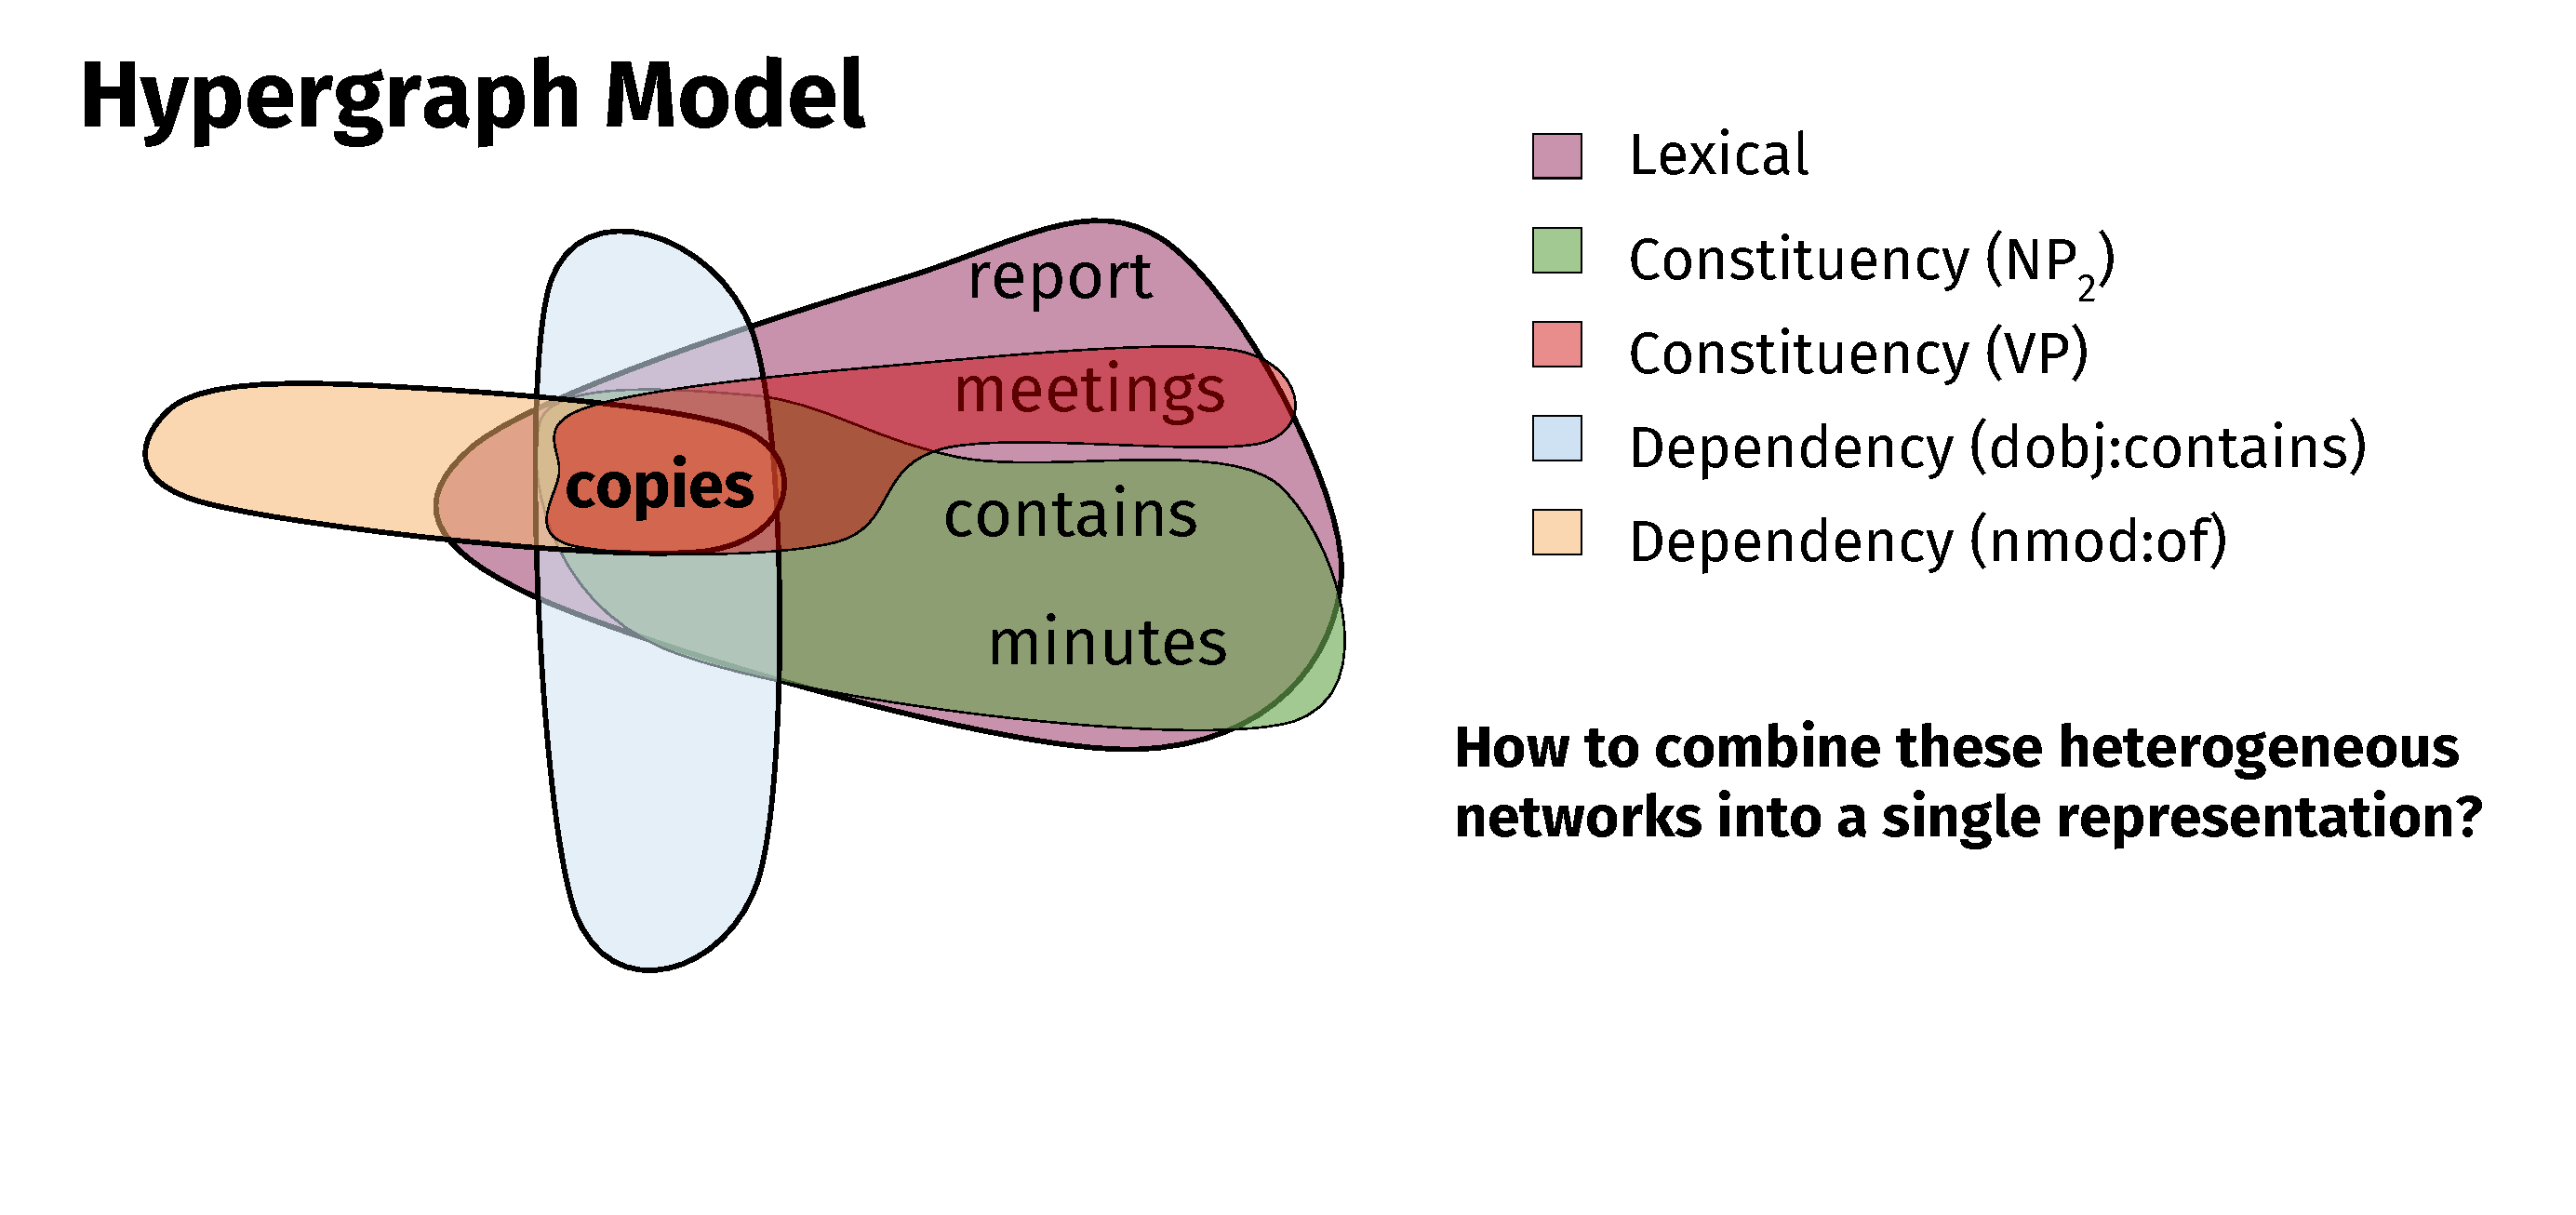
\includegraphics[width=1\linewidth]{image2/Chapitre2/hyper_network_ex_6.pdf}%dep
	
	\begin{itemize}
	\item[] How to combine these networks together?
	\end{itemize}
	\end{overprint}
	\vspace{7cm}
	\pnote{YOU SHOULD BE 12 MINS}
\end{frame}

%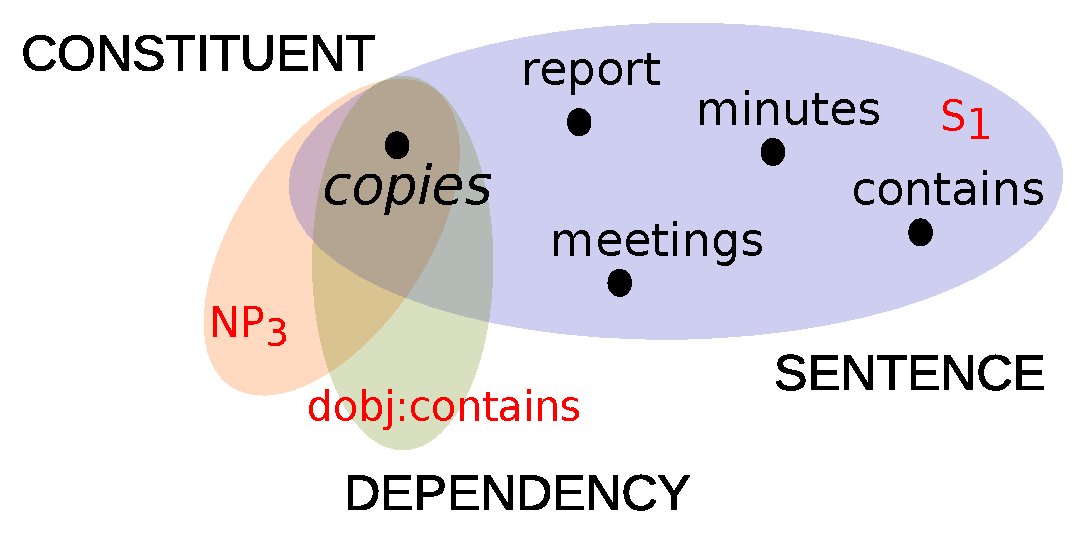
\includegraphics[width=.6\linewidth]{img/hypergraph_copies.pdf} <===== THIS!

\setbeamertemplate{section page}[mytheme]
\section[Contributions in Detail]{Combining Features and Dealing with Sparsity}                  

      
\begin{frame}{Multimedia Fusion Techniques}
\vfill
%\vspace{.5cm}
\begin{itemize}
\item<1-> \large \textbf{Definition}
	\begin{itemize}
	\item<1-> Used in multimedia analysis tasks to integrate multiple media 
	\item<1-> We adapt them to combine textual information

	\item<1-> The goal is to obtain rich insights about the data being treated
	\item<1-> By creating a single representation from heterogeneous information
	\end{itemize}									
\vfill	
\item<2-> \large\textbf{Main fusion operators:}
	\begin{itemize}
	\item<2-> Early Fusion $E_\alpha(\cdot)$, 
	\item<2-> Late Fusion $L_\beta(\cdot)$, 
	\item<2-> Cross Fusion $X_\gamma(\cdot)$
%	\item $\alpha$ and $\beta$: Assign an importance weight to each of their operators 
%	\item $\gamma$: number of top similar items to take from the similarity space
	\end{itemize}

\end{itemize}
\hfill
\end{frame}




\begin{frame}{Early and Late Fusion}
\centering
\onslide<1->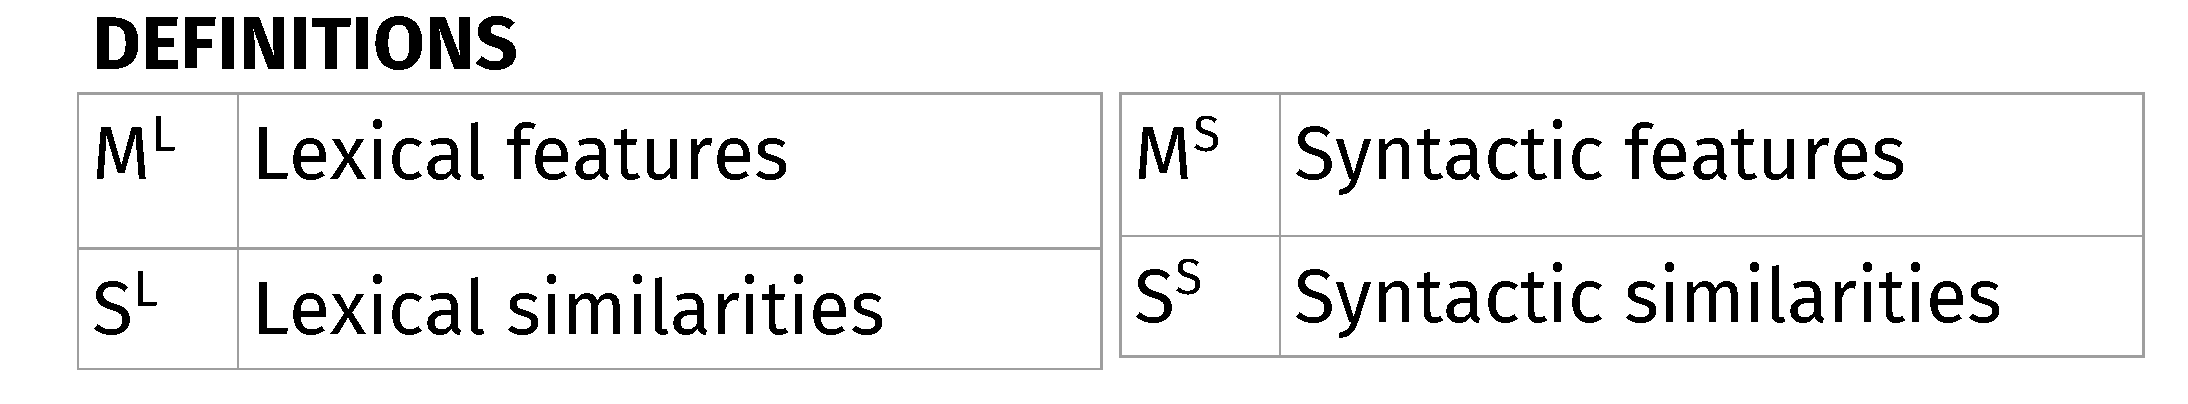
\includegraphics[width=.8\linewidth]{image2/Chapitre3/definition_S_L.pdf}
\vfill
\begin{columns}
	\column{0.5\textwidth}
	\begin{minipage}[c][0.5\textheight][c]{\linewidth}
		\centering
		\onslide<1->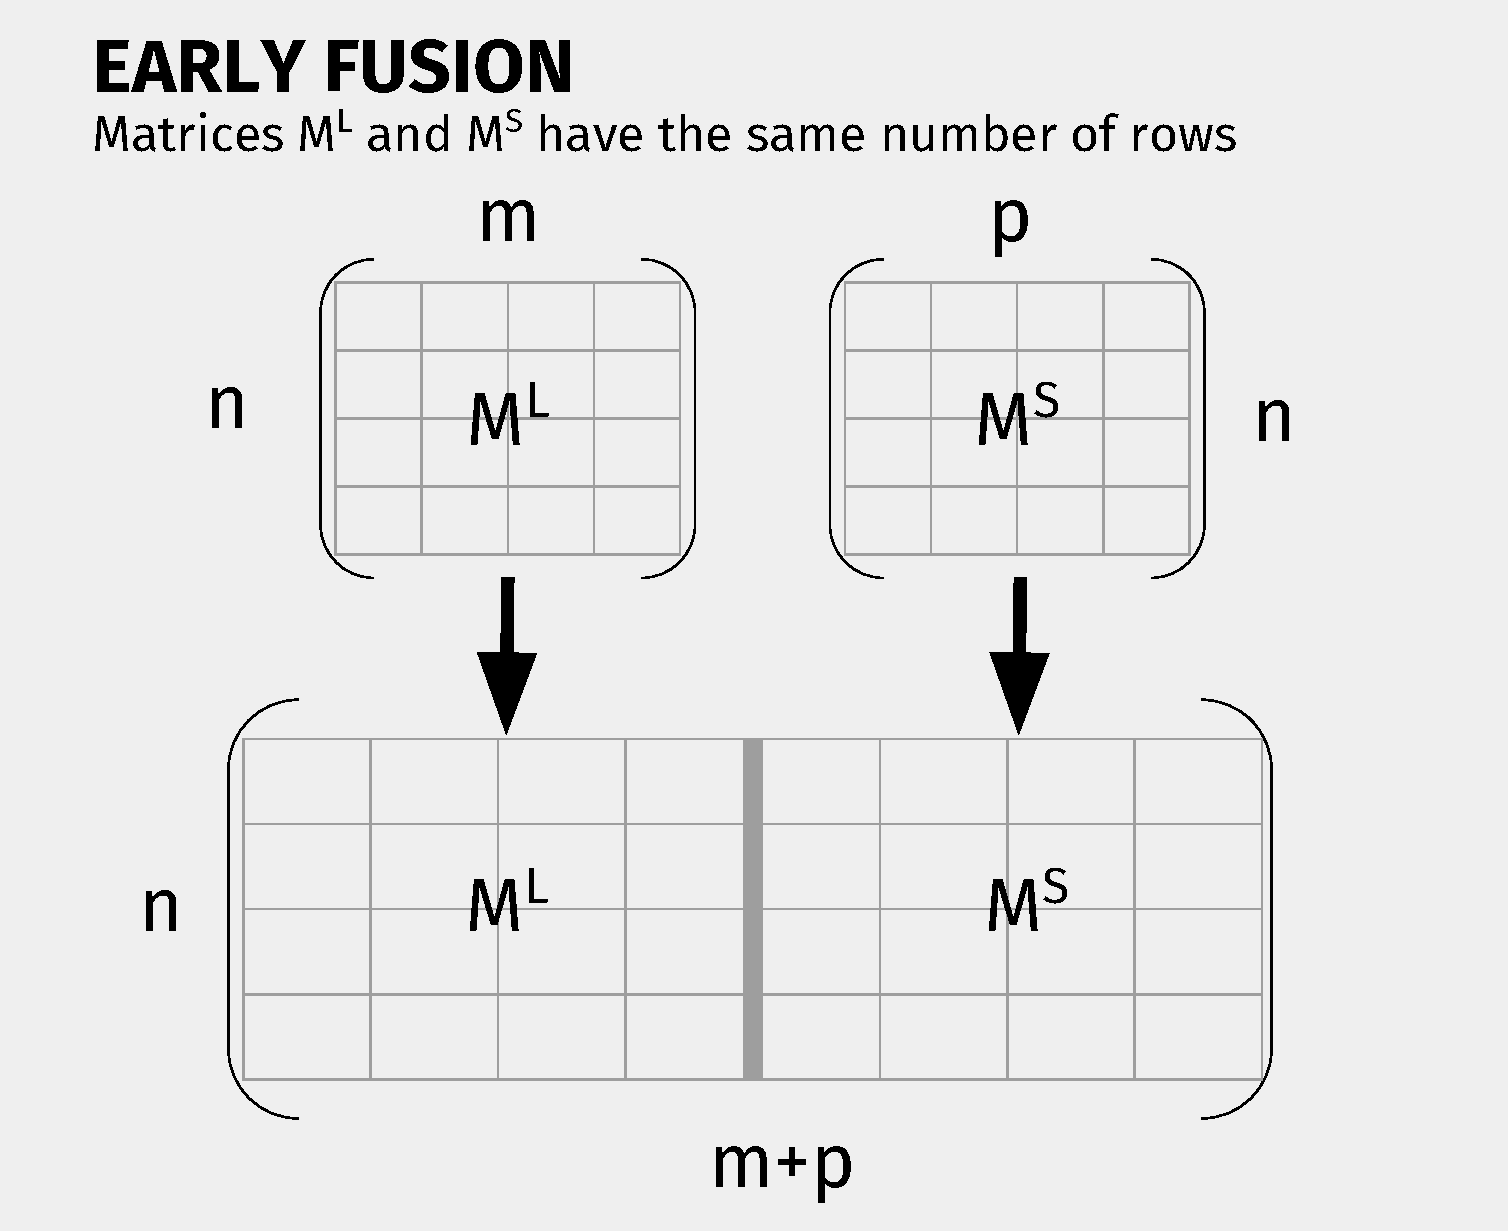
\includegraphics[width=1\linewidth]{image2/Chapitre3/ef_diag}
		\end{minipage}
		\column{0.5\textwidth}
	\begin{minipage}[c][0.5\textheight][c]{\linewidth}
		\centering
		\onslide<2->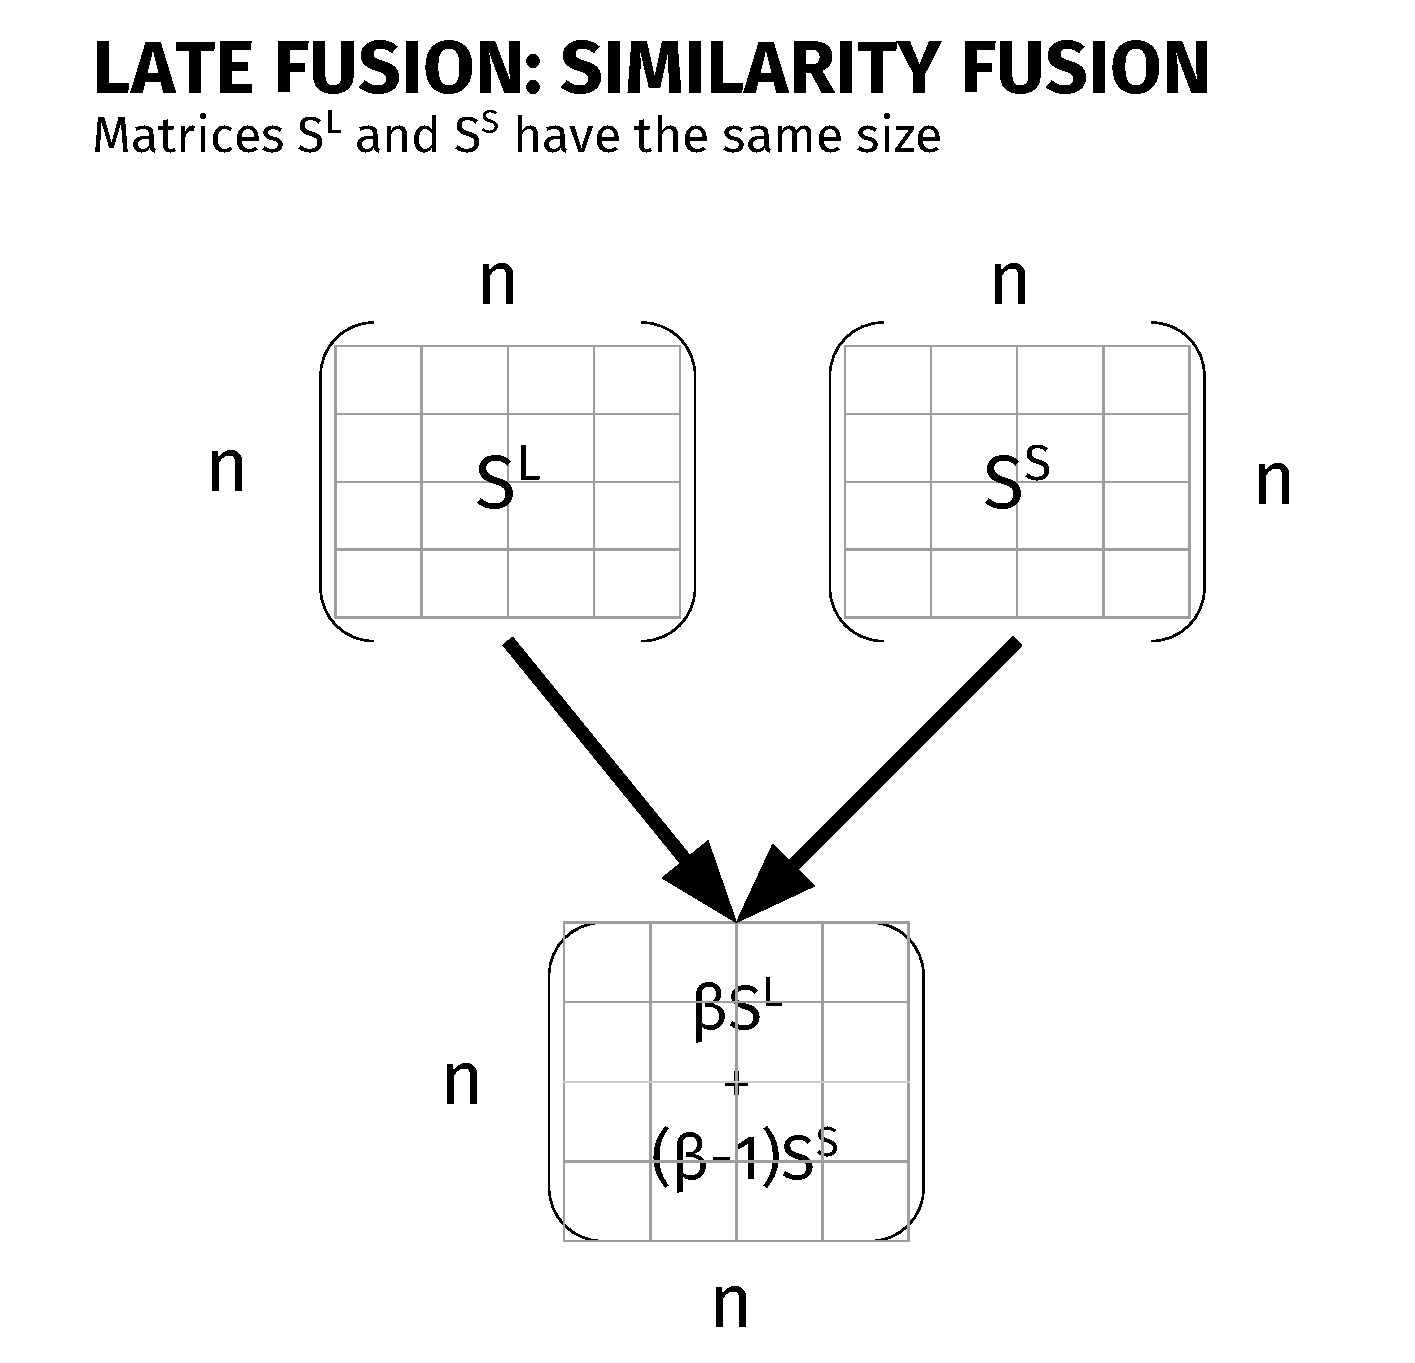
\includegraphics[width=1\linewidth]{image2/Chapitre3/lf2_diag.pdf}
	\end{minipage}
\end{columns}




\end{frame}



\begin{frame}{Cross Fusion}
\begin{center}
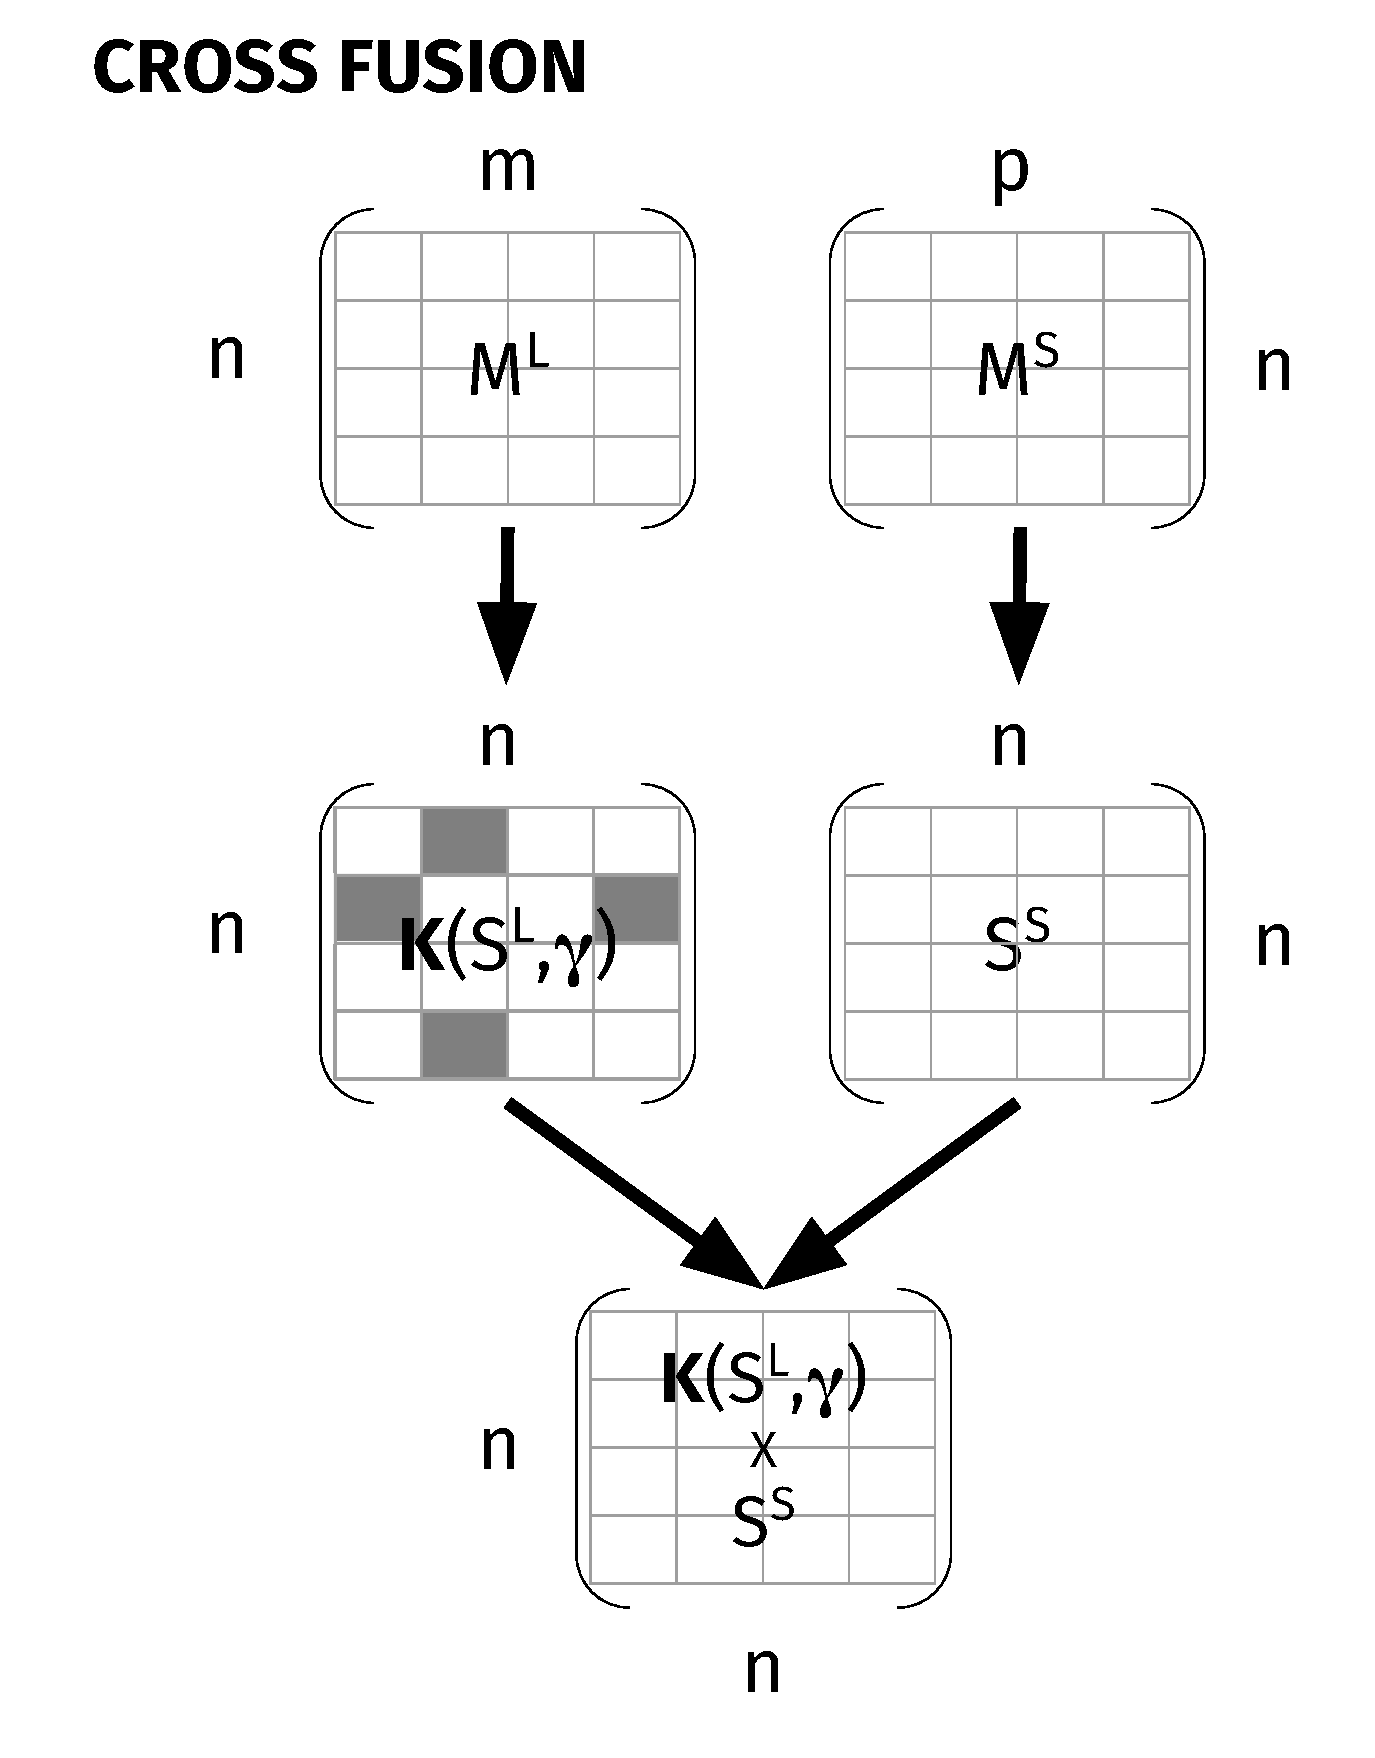
\includegraphics[width=.55\linewidth]{image2/Chapitre3/xf_diag.pdf}
\end{center}
\end{frame}


\begin{frame}{Hybrid Fusion}
\begin{itemize}
%\item \large Combining fusion operators
%	\begin{itemize}
%	\item Chaining together fusion functions to leverage the complementarity of the different features
%	\end{itemize}
\item<1-> \textbf{Combining fusion operators}

\begin{itemize}
\item<1-> Applying one function to the result of another to produce a new fusion function
\end{itemize}
\begin{overprint}
	\onslide<2>
		\begin{itemize}
		\item \textbf{First Degree} 
			\begin{itemize}
			\item $E(\mlex,\msyn)$, $L(\ssyn,\mlex)$ 
			\item \textbf{Cross Feature Fusion}: $X_F(S^S, M^L)$
			\item \textbf{Cross Similarity Fusion}: $X_S(S^S, S^L)$
			\end{itemize}
		\end{itemize}
		\centering
		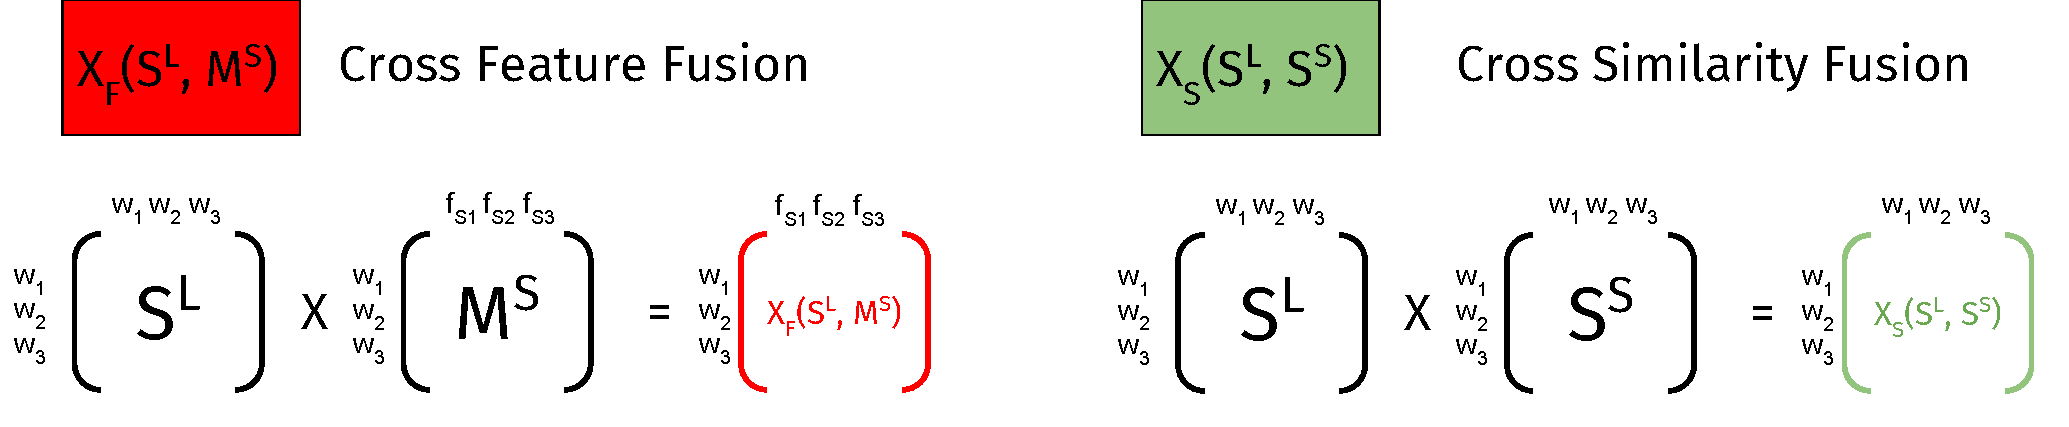
\includegraphics[width=1\linewidth]{image2/Chapitre2/xFFusion.pdf}
	\onslide<3>
		\begin{itemize}
		\item \textbf{Second Degree} 
			\begin{itemize}
			\item \textbf{Cross Feature Early Fusion}: $X_F(S^T , E(M^S, M^L ))$
			\item \textbf{Late Cross Feature Fusion}: $L(M^T, X_F (S^T , M^T ))$
			\end{itemize}
		\end{itemize}
		\centering
		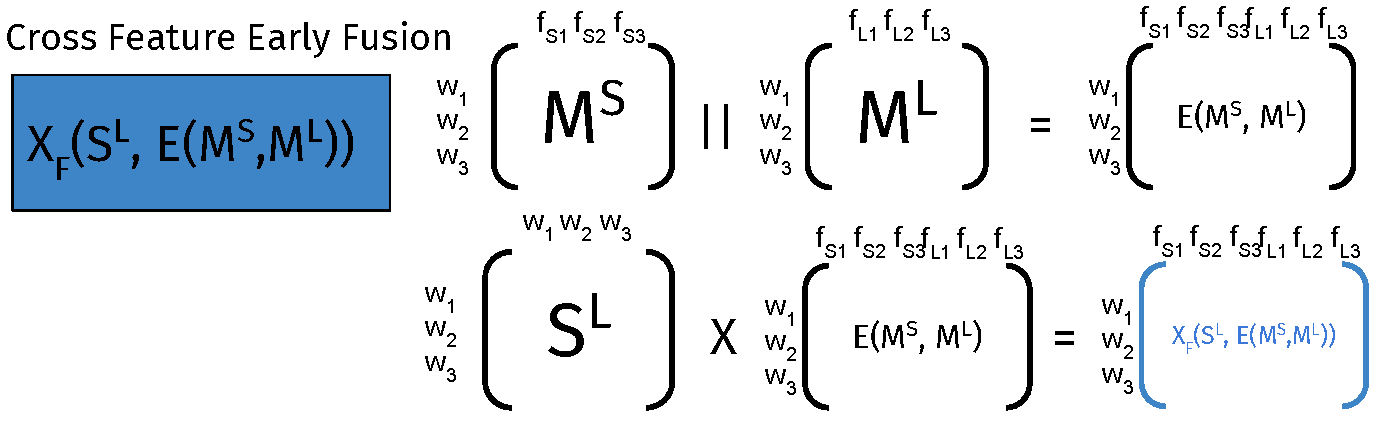
\includegraphics[width=1\linewidth]{image2/Chapitre2/XFEF.pdf}

	\onslide<4>
		\begin{itemize}
		\item \textbf{Higher Degree}
			\begin{itemize}
			\item Triple Early Double Late Cross Feature Fusion: $E(M_L , E(E(M_T , L(M^T , X_F (S^T , M^T ))) , L(M^L , X_F (S^S , M^L))))$
			\end{itemize}
		\end{itemize}
		
\end{overprint}
	

\end{itemize}
\vfill
\end{frame}

\begin{frame}{High Degree Fusion}
\begin{itemize}
\item[] \large \textbf{Higher Degree Operator }
\end{itemize}
\begin{overprint}
	\onslide<1>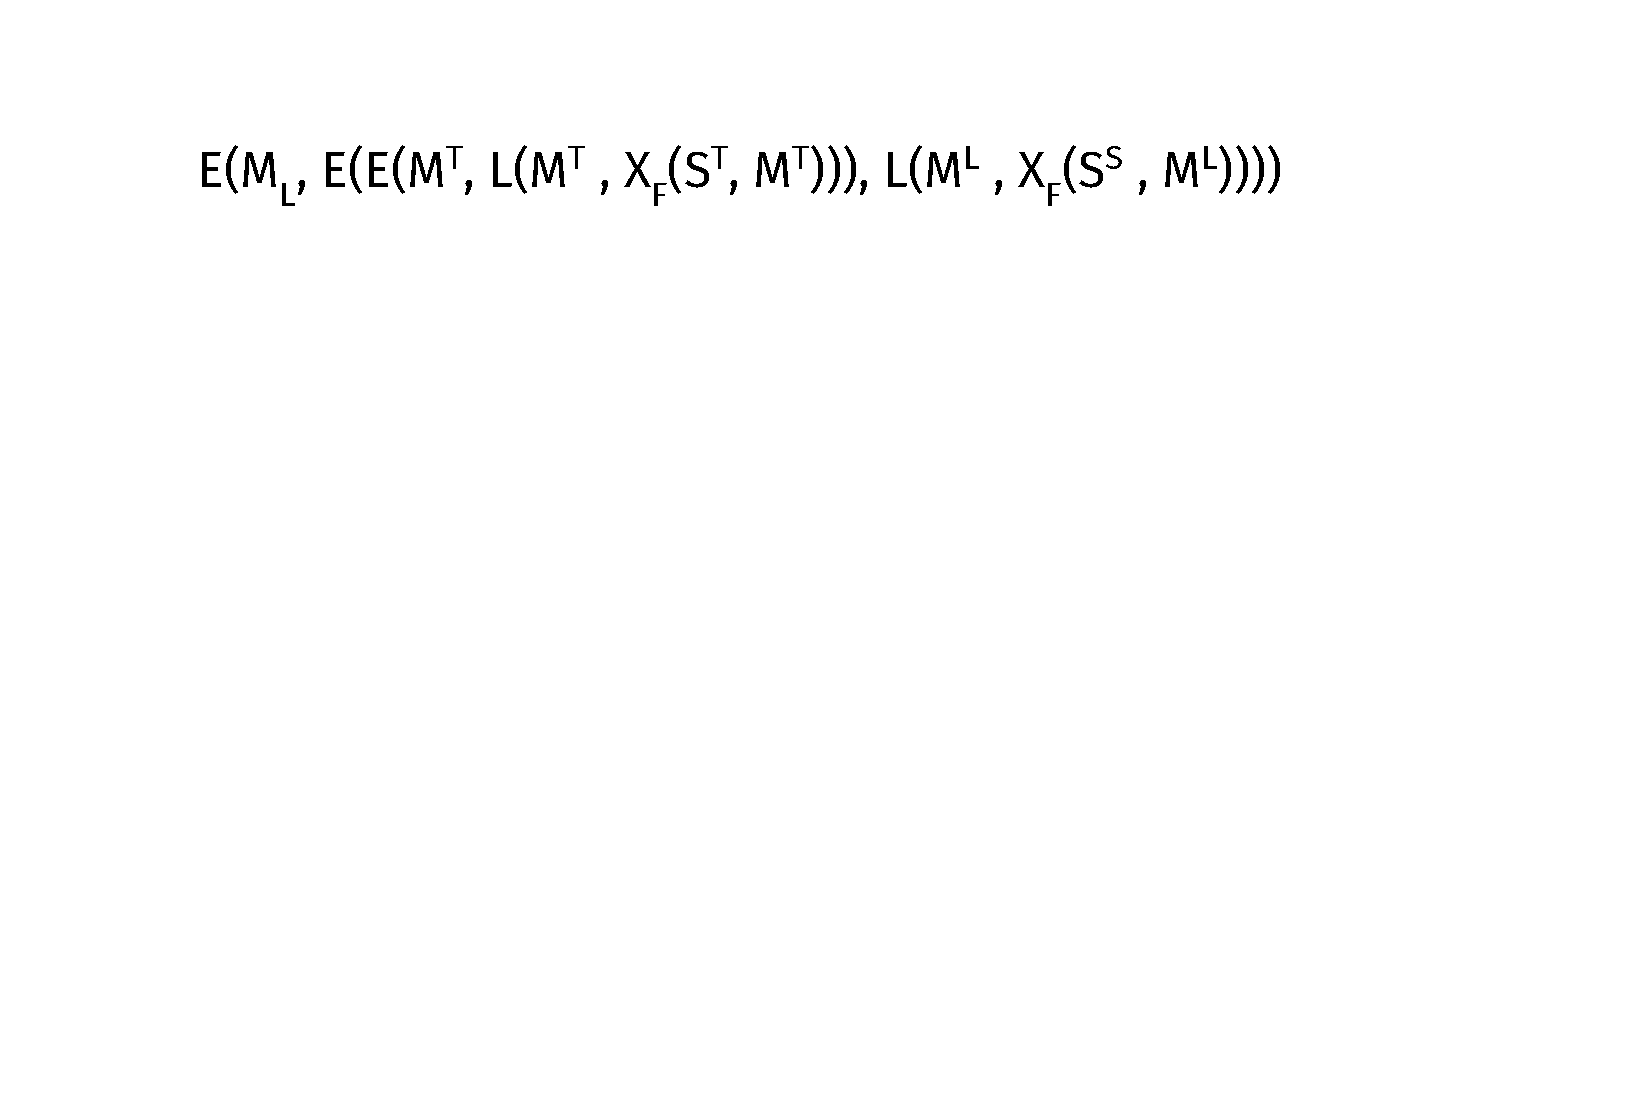
\includegraphics[width=1\linewidth]{image2/Chapitre2/hybrid_fusion0.pdf}%lexical
	\onslide<2>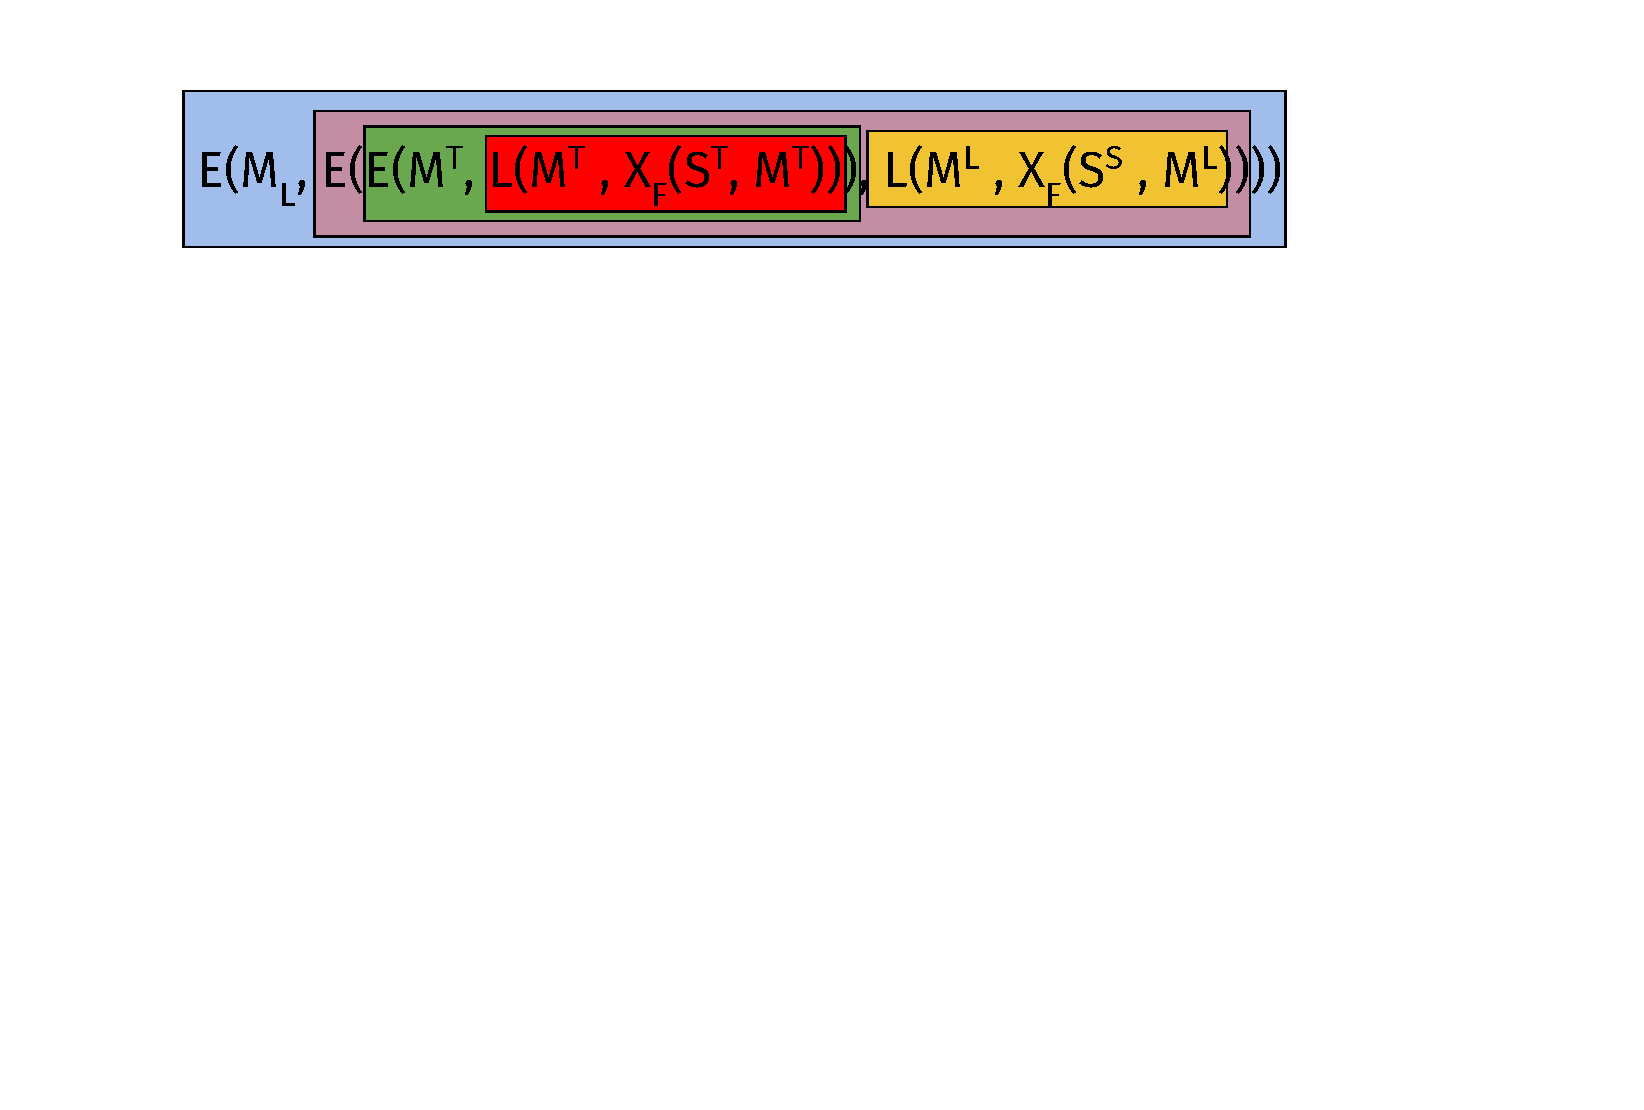
\includegraphics[width=1\linewidth]{image2/Chapitre2/hybrid_fusiona.pdf}%lexical
	\onslide<3>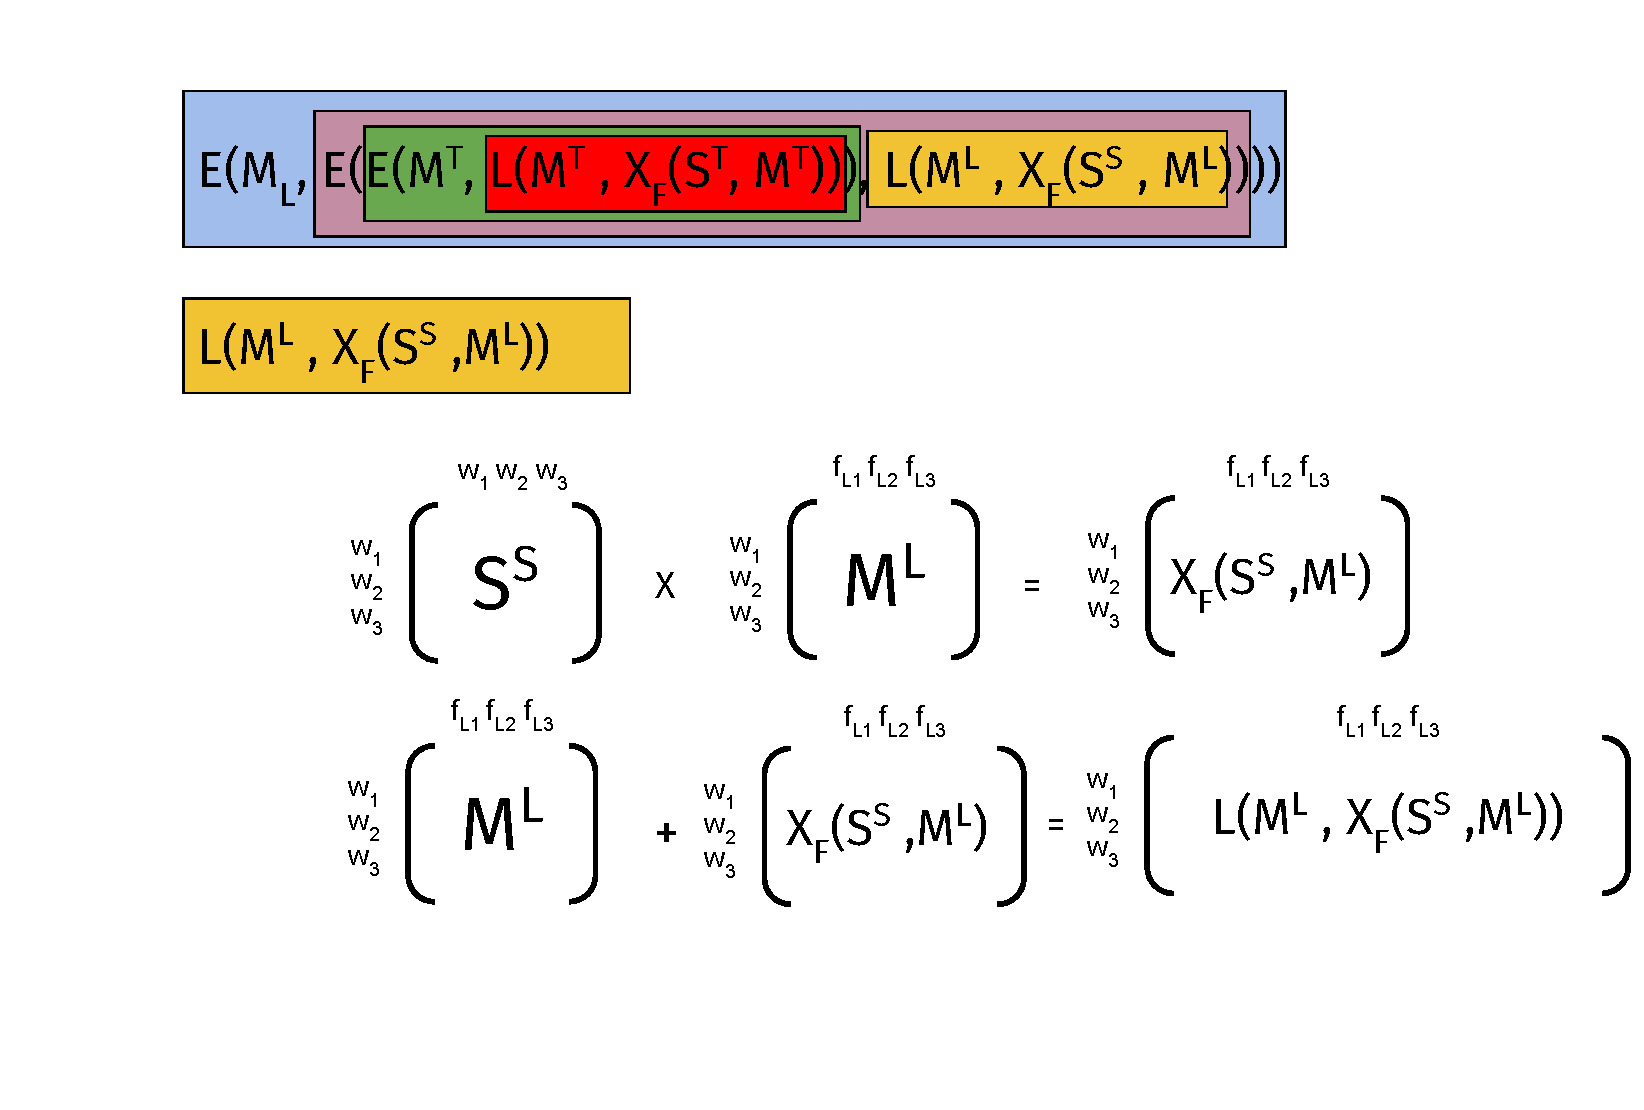
\includegraphics[width=1\linewidth]{image2/Chapitre2/hybrid_fusion1.pdf}%lexical
	\onslide<4>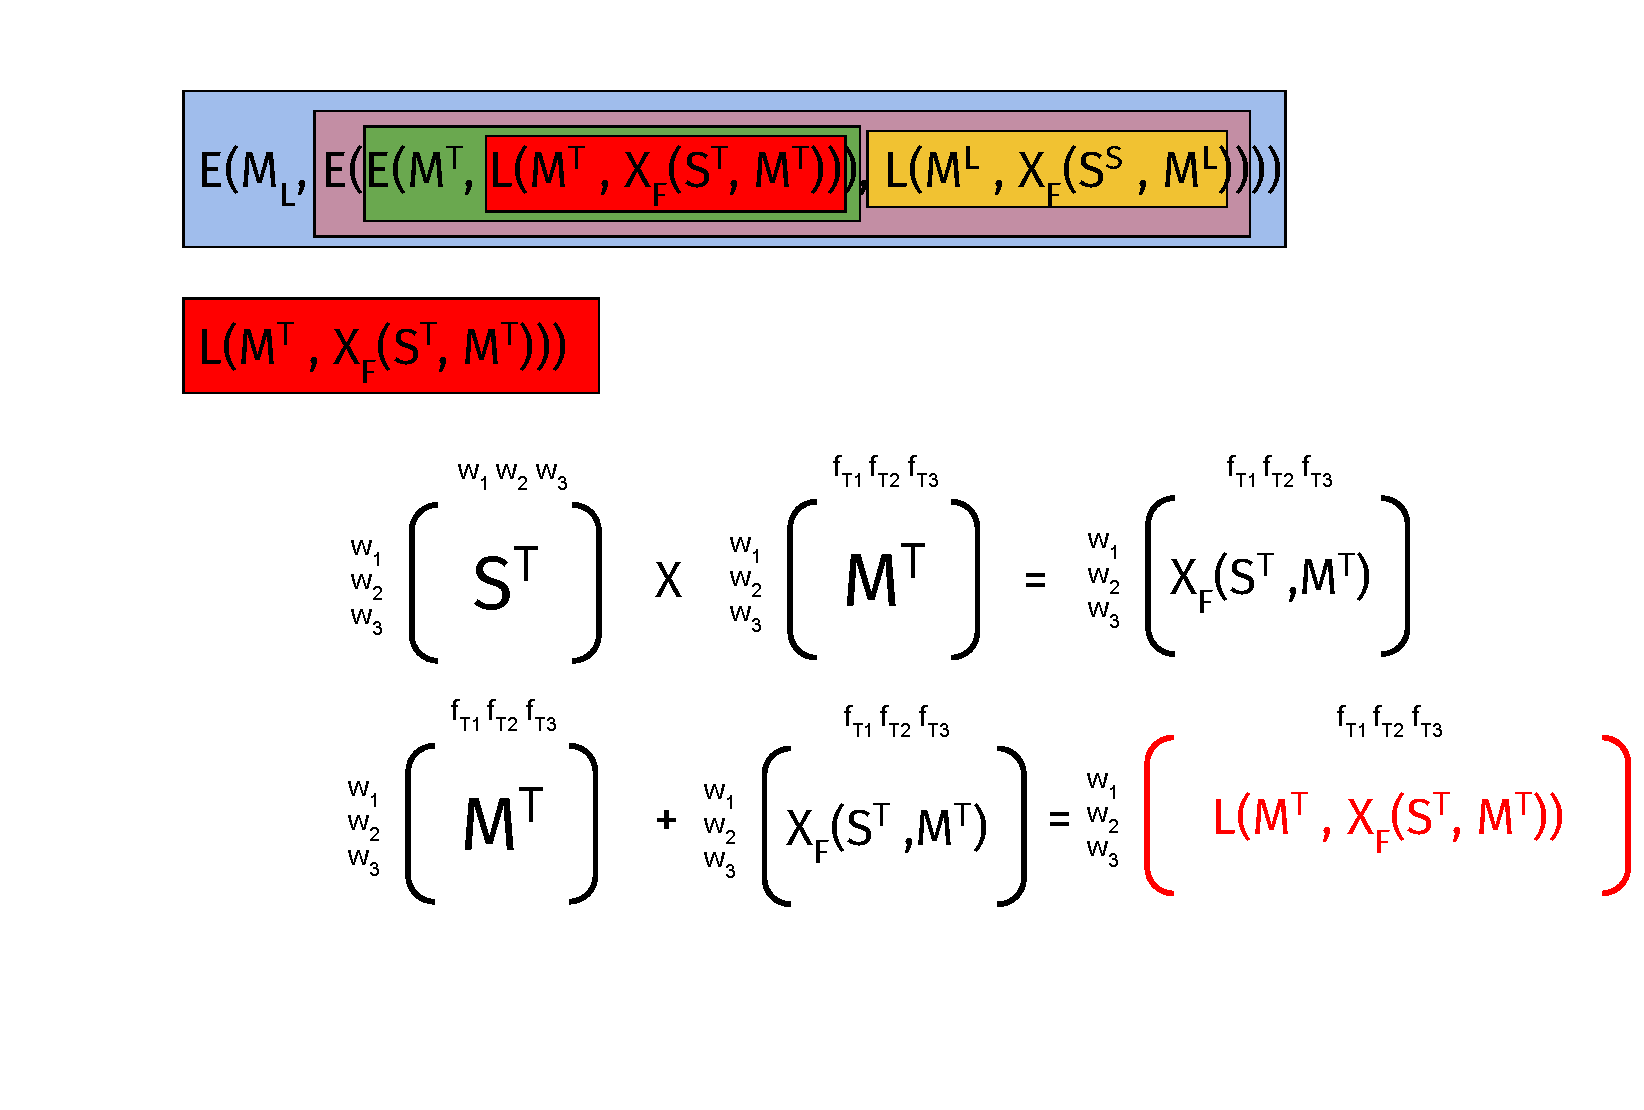
\includegraphics[width=1\linewidth]{image2/Chapitre2/hybrid_fusion2.pdf}%constit
	\onslide<5>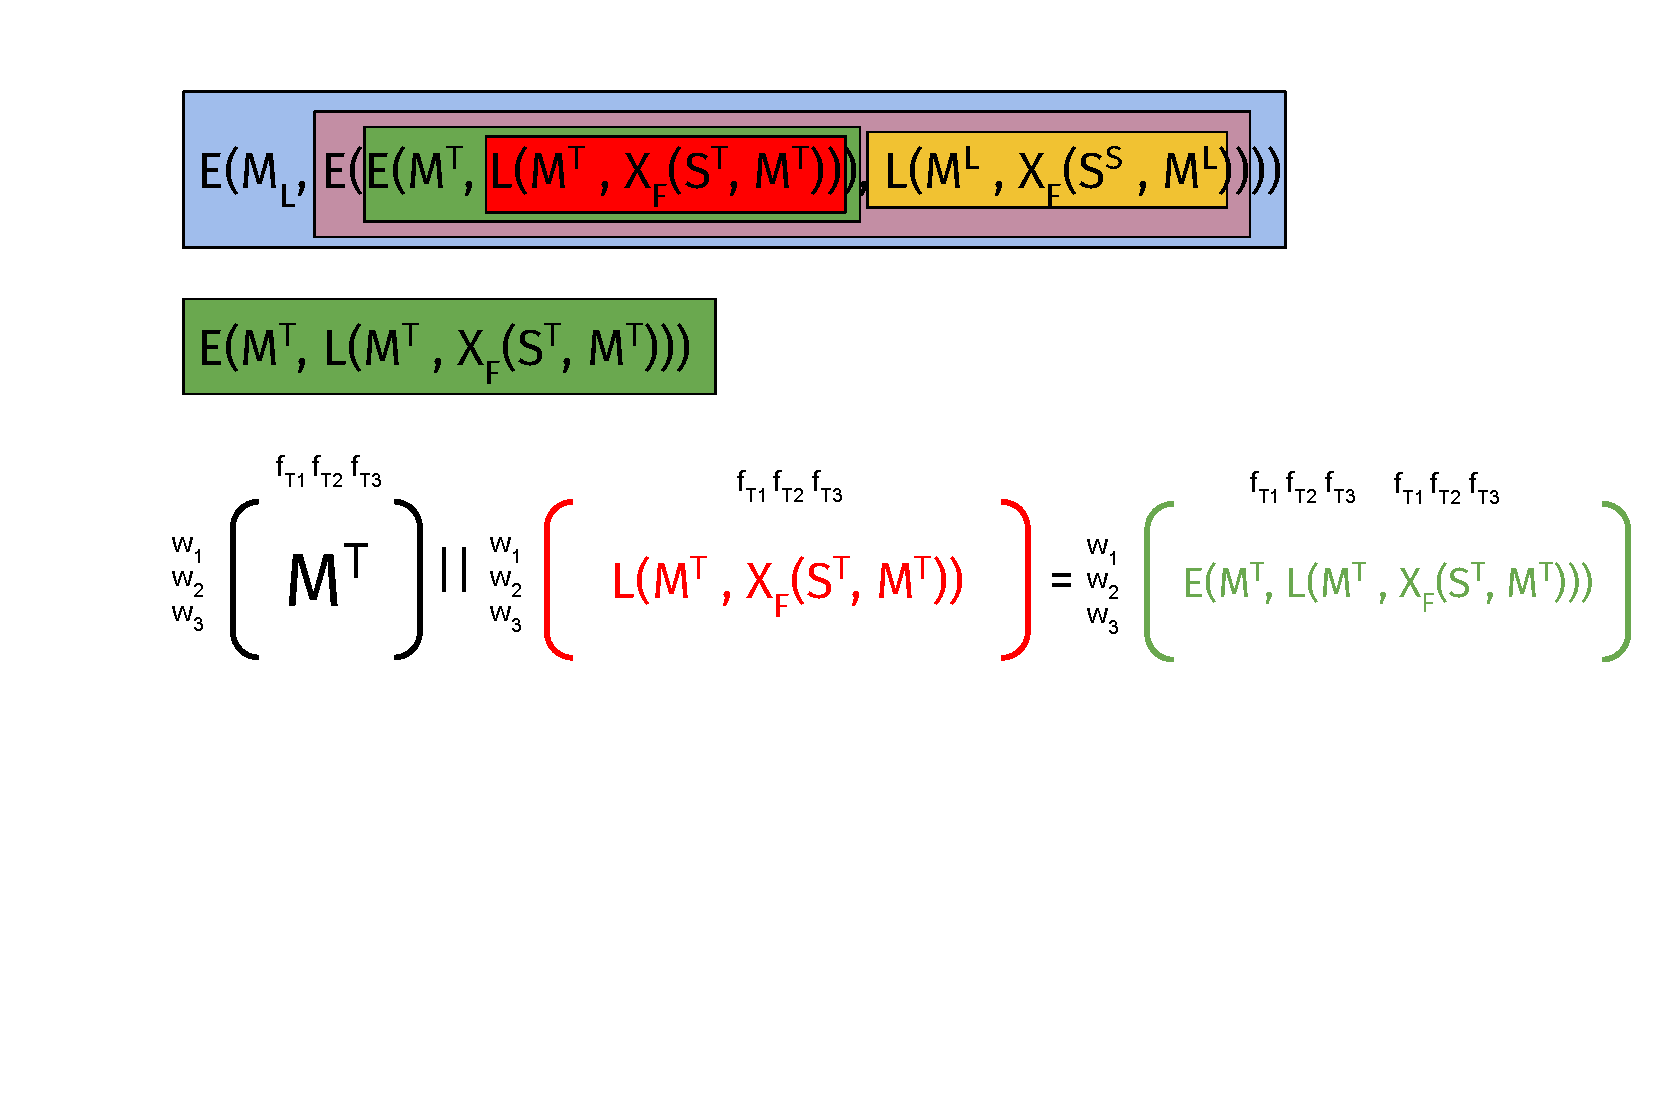
\includegraphics[width=1\linewidth]{image2/Chapitre2/hybrid_fusion3.pdf}%constit
	\onslide<6>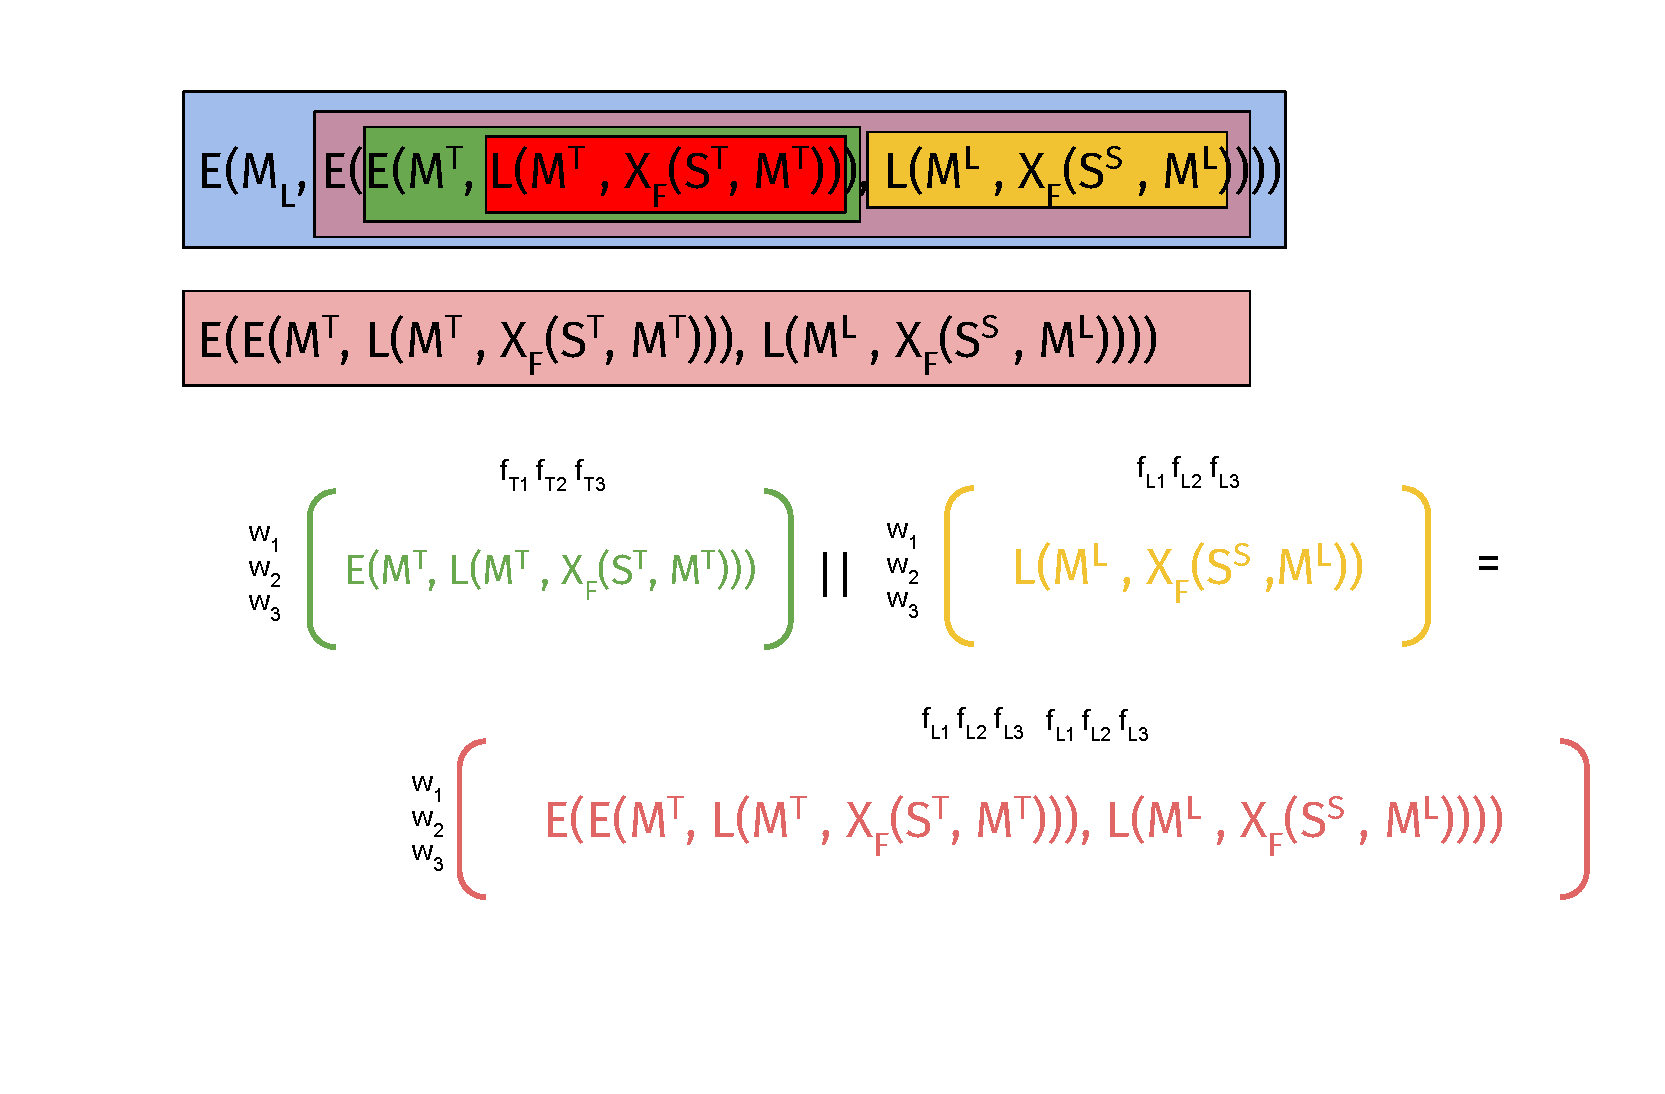
\includegraphics[width=1\linewidth]{image2/Chapitre2/hybrid_fusion4_a.pdf}%dep
	\onslide<7>\includegraphics[width=1\linewidth]{image2/Chapitre2/hybrid_fusion4.pdf}%dep
\end{overprint}
\end{frame}






\section[Contributions in Detail]{Finding Communities in the Network}


\begin{frame}{Introduction}

	\begin{itemize}
		\item<1-> \large \textbf{Language networks tend to be scale-free}	
			\begin{itemize}
				\item<1-> There are certain nodes (hubs) that are very well connected forming communities within the network
			\end{itemize}
%
		\item<2-> \large \textbf{Seminal approaches}
			\begin{itemize}
				\item<2-> Hyperlex \cite{2004.Veronis}
				\item<2-> University of York (UoY) \cite{2007.Klapaftis.UOY}
			\end{itemize}
		\item<3-> \textbf{Limitations of existing approaches}
		\begin{itemize}
			\item<3-> Single typed networks
			\item<3-> Large number of parameters
		\end{itemize}
		\item<4-> \textbf{Proposition}
		\begin{itemize}
				\item<4-> Be able to exploit different types of linguistic information (lexical or syntactic co-occurrence)
				\item<4-> Keep  the number of parameters low and allow for their automatic adjusting according to the network's nature
%				\item Use a robust and interpretable similarity measure
		
		\end{itemize}
\end{itemize}
\vspace{\textheight}	
\end{frame}
\begin{frame}{Proposed Method}
  \centering
  \includegraphics[width=1\linewidth]{img/wsd_wsi.png}

\end{frame}


\begin{frame}<presentation:0>[noframenumbering]{Leveraging the network communities} 
\begin{enumerate}
\item Link some words together with a color overlay to represent possible communities (clusters/groups) of same sense words. 
\item Argue that thanks to the heterogeneous info contained in the structure, we can relate words according to different linguistic properties 

\end{enumerate}
\end{frame}

\section[Applications to NLP]{Hypergraph Model Instantiation}



\begin{frame}<presentation:0>[noframenumbering]{Introduction}
\large \textbf{Applications}
\vspace{.5cm}
\begin{itemize}
\item \large \textbf{We instantiate our proposed linguistic resource}
\begin{itemize}
\item Based on the English Wikipedia corpus
\end{itemize}
\item \large \textbf{Use the proposed model  to solve two NLP tasks}
	\begin{itemize}
	\item Named Entity Recognition 
	\item Word Sense Induction and Disambiguation
	\end{itemize}
\vspace{.3cm}
\item \large \textbf{These experiments have two main objectives}
	\begin{itemize}
	\item Test the effectiveness of fusion enriched representations (heterogeneity + less sparse spaces)
	\item Leverage the structure of the network built following our proposed model
	\end{itemize}

\end{itemize}
\vspace{\textheight}
\end{frame}

\subsection{Introduction}
\begin{frame}{Hypergraph Model Instantiation}
\begin{itemize}
\item<1-> \large \textbf{Apply our proposed linguistic model to a real world corpus}
	\begin{itemize}
	\item<1-> Use the English Wikipedia as input and generate a textual structure following the proposed network model
	\end{itemize}
%\item<2-> \large \textbf{We provide two resources}
%\begin{itemize}
%	\item<2-> A syntactically annotated English Wikipedia corpus (SAEWD)
%	\item<2-> A Wikipedia-based enriched hypergraph linguistic model 
%\end{itemize}
\item<2-> \large \textbf{Steps performed}	
\begin{itemize}
	\item<2->[] \begin{center}
		\includegraphics[width=\linewidth]{image2/Chapitre7/saewd}
		\end{center}

\end{itemize}

\end{itemize}

\end{frame} 


\begin{frame}<presentation:0>{Syntactically Annotated Wikipedia}


			 	\centering	           
	\adjustbox{max height=\dimexpr\textheight-6.5cm\relax,
	           max width=\textwidth}{
\begin{tabular}{llllll}
 \multicolumn{6}{l}{\textit{FILENAME wiki\_00.parsed}}                                           \\ \hline
  \textbf{token}   & \textbf{lemma}   & \textbf{POS} & \textbf{constituency}                      & \textbf{head} & \textbf{dependency} \\ \hline
 \multicolumn{6}{l}{\textit{\%\%\#PAGE Anarchism}}                                         \\ \hline
  {$\vdots$}      &      {$\vdots$}   &  {$\vdots$}   &     {$\vdots$}                              &    {$\vdots$}  &     {$\vdots$}       \\  \hline
 \multicolumn{6}{l}{\textit{\%\%\#SEN 25  9}}                                             \\ \hline
						 A       & a       & DT  & NP\_22,S\_97                      & 3    & det        \\ %\cline{2-7} 
                         great   & great   & JJ  & NP\_22,S\_97                      & 3    & amod       \\ %\cline{2-7} 
                         brigand & brigand & NN  & NP\_22,S\_97                      & 4    & nsubj      \\ %\cline{2-7} 
                         becomes & become  & VBZ & VP\_44,S\_97                      & 0    & root       \\ %\cline{2-7} 
                         a       & a       & DT  & NP\_18,NP\_20,VP\_44,S\_97        & 6    & det        \\ %\cline{2-7} 
                         ruler   & ruler   & NN  & NP\_18,NP\_20,VP\_44,S\_97        & 4    & xcomp      \\ %\cline{2-7} 
                         of      & of      & IN  & PP\_57,NP\_20,VP\_44,S\_97        & 9    & case       \\ %\cline{2-7} 
                         a       & a       & DT  & NP\_18,PP\_57,NP\_20,VP\_44,S\_97 & 9    & det        \\ %\cline{2-7} 
                         Nation  & nation  & NN  & NP\_18,PP\_57,NP\_20,VP\_44,S\_97 & 6    & nmod       \\ %	\cline{2-7} 
\hline 
\end{tabular}}

\end{frame}


\begin{frame}{Hypergraph Incidence Matrix}
\begin{center}
\includegraphics[width=1\linewidth]{img/incidence_aug.pdf}
\end{center}

\end{frame} 



\begin{frame}{Wikipedia Feature Enriched Space}
%\textbf{Target word \textit{priest} and its top 5 most similar words using different representation matrices.}
\begin{itemize}
	\item \textbf{Characteristics of the enriched space}
	\begin{itemize}
	\item Sparsity is reduced
	\item Semantic relatedness differs according to the representation space
	\end{itemize}
\end{itemize}
\begin{tabular}{@{}llllll@{}}
\toprule
                           & \textbf{\begin{tabular}[c]{@{}l@{}}Lexical\\ Features\\ \textcolor{orangeEric}{(5.49\%)}\\$\mlex$\end{tabular}}              
                           & \textbf{\begin{tabular}[c]{@{}l@{}}Syntactic\\ Features\\(4.97\%)\\$\msyn$\end{tabular}}        
                           & \textbf{\begin{tabular}[c]{@{}l@{}}Early\\ Fusion\\(5.23\%)\\$E(\mlex, \msyn)$\end{tabular}}                
                           & \textbf{\begin{tabular}[c]{@{}l@{}}$X_F$\\Fusion\\\textcolor{red}{(16.75\%)}\\$X_F(\ssyn, \mlex)$\end{tabular}}   &
                           \textbf{\begin{tabular}[c]{@{}l@{}}$X_F$\\Fusion\\ (13.45\%) \\$X_F(\slex, \msyn)$\end{tabular}}                 \\ \midrule
\multicolumn{1}{c}{\textbf{priest}} & \begin{tabular}[c]{@{}l@{}}priests\\ nun\\ canton\\ sailor\\ burial\end{tabular} & \begin{tabular}[c]{@{}l@{}}monk\\ regent\\ aedile\\ seer\\ meek\end{tabular} & \begin{tabular}[c]{@{}l@{}}sailor\\ regent\\ nuclei\\ nun\\ relic\end{tabular} & \begin{tabular}[c]{@{}l@{}}vassal\\ regent\\ nun\\ sailor\\ monk\end{tabular} & \begin{tabular}[c]{@{}l@{}}sailor\\ fluent\\ dean\\ nuclei\\ chorus\end{tabular} \\

 \bottomrule
\pnote{!!YOU SHOULD BE ~22 mins!!!}
\end{tabular}
\end{frame}

%\begin{frame}{Wikipedia Similarity Enriched Spaces}
%\smaller
%\begin{tabular}{@{}lllllll@{}}
%\toprule
%                           & \textbf{\begin{tabular}[c]{@{}l@{}}Lexical\\ Similarity\\(75.25\%)\\$S^L$\end{tabular}}              & \textbf{\begin{tabular}[c]{@{}l@{}}Syntactic\\ Similarity\\(60.64\%)\\$S^S$\end{tabular}}        & \textbf{\begin{tabular}[c]{@{}l@{}}Early\\ Fusion\\(67.94\%)\\$E(S^L, S^S)$\end{tabular}}                & \textbf{\begin{tabular}[c]{@{}l@{}}Late\\ Fusion\\(83.17\%)\\$L(S^L, S^S)$\end{tabular}}                 & \textbf{\begin{tabular}[c]{@{}l@{}}$X_S$\\ Fusion\\(87.22\%)\\$X_S(\ssyn, \slex)$\end{tabular}}  &
%                           \textbf{\begin{tabular}[c]{@{}l@{}}$X_S$\\
%                           Fusion\\(79.69\%)\\$X_S(\slex,\ssyn)$\end{tabular}}                 
%                           \\ \midrule
%\multicolumn{1}{c}{\textbf{priest}} 
%& \begin{tabular}[c]{@{}l@{}}wholly\\burial\\monk\\lingua\\nuclei\end{tabular} &
%\begin{tabular}[c]{@{}l@{}}regent\\ coach\\ broker\\ dream\\tailor\end{tabular} & \begin{tabular}[c]{@{}l@{}}regent\\slang\\ broker\\rebel\\tiger\end{tabular} & \begin{tabular}[c]{@{}l@{}}regent\\slang\\ seer\\ tutor\\cradle\end{tabular} & \begin{tabular}[c]{@{}l@{}}regent\\vassal\\vizier\\leader\\result\end{tabular} & \begin{tabular}[c]{@{}l@{}}sailor\\nuclei\\nun\\canton\\burial\end{tabular} \\
%
% \bottomrule
%
%\end{tabular}
%\end{frame}

\section[Applications to NLP]{Solving Named Entity Recognition}



\begin{frame}{Introduction}
\begin{itemize}
\item<1-> \large \textbf{NER Objective}
\begin{itemize}
\item<1->  The goal is to automatically discover  mentions that belong to a well-defined semantic category. 

\end{itemize}
\item<2-> \large \textbf{Classic entities types}
	\begin{itemize}
	\item<2-> Location (LOC)
	\item<2-> Organization (ORG)
	\item<2-> Person (PER)
	\item<2-> Miscellaneous (MISC)
	\item<2-> None (O)
	\end{itemize}
\item<3-> \large \textbf{Our goal}
\begin{itemize}
\item<3-> We assess the effectiveness of the classic fusion methods and propose new hybrid combinations 
\end{itemize}

\end{itemize}
\end{frame}

%
%\begin{frame}{Experiment Flow Diagram}
%\centering
%\includegraphics[width=0.85\linewidth]{image2/Chapitre4/diag_metodoNER.pdf}
%\end{frame}


\begin{frame}{Representation Spaces}
\hfill
\begin{itemize}
	\item[] \large \textbf{Example Phrase}
	\begin{itemize}
	\item[] \large \textit{Australian scientist discovers star with telescope}
	\end{itemize} 
\end{itemize}
\hfill
\begin{itemize}
\item[] \large \textbf{Three different types of features}
\end{itemize}

\small

\begin{tabular}{llr}

	\hline 
	 \textbf{Word} & \textbf{Features} & \textbf{Feature Type}\\ 
	\hline 
	\rowcolor{greenEric!70}	
	Australian & word:Australian, word+1:scientist, ...& \textbf{Lexical (L)}\\ 
	\rowcolor{orangeEric!70}	
	scientist  &  Australian/JJ/amod, discovers/VBZ/nsubj\_inv & \textbf{Syntactic (S)}\\ 
	\rowcolor{blue!30}
	discover &discover, no-capital-letter, prf:dis, suf:ver, VBZ & \textbf{Standard (T)}\\ 
	\hline 
\end{tabular} 
\vspace{\textheight}
\end{frame}


%\begin{frame}{Representation Spaces}
%	\large \textbf{Syntactic Space (S)}
%	\vspace{1cm}
%	\small
%	
%	
%	\begin{tabular}{ll}
%	\hline 
%	 Word & Contexts \\ 
%	\hline 
%	Australian & scientist/NN/amod\_inv \\ 
%	scientist  &  Australian/JJ/amod, discovers/VBZ/nsubj\_inv\\ 
%	discovers & scientist/NN/nsubj, star/NN/dobj, telescope/NN/nmod:with \\ 
%	star & discovers/VBZ/dobj\_inv \\ 
%	telescope  &  discovers/VBZ/nmod:with\_inv \\ 
%	\hline \
%	\end{tabular} 
%	 
%	\vspace{\textheight}
%\end{frame}
%


%\begin{frame}{Representation Spaces}
%	\large \textbf{Standard Features Space (T)}
%	\vspace{1cm}
%	\begin{itemize}
%		\item Each word
%		\item Whether it is capitalized
%		\item Prefix and suffix (of each word their surroundings)
%		\item Part of Speech tag
%	\end{itemize}	 
%	\vspace{\textheight}
%\end{frame}



\begin{frame}{Experimental Protocol}
	\begin{itemize}
		\item<1-> \large \textbf{Preprocessing}
			\begin{itemize}
				\item<1-> Normalize numbers
			\end{itemize}
		\item<2-> \textbf{Test Corpora}
			\begin{itemize}
			\item<2-> CoNLL-2003 (CONLL): Train: 219,554 lines. Test: 50,350 lines
			\item<2-> Wikiner (WNER): 3.5 million words. 
			\item<2-> Wikigold (WGLD): 41,011 words. 
			\end{itemize}
		\item<3-> \textbf{Learning Algorithm}
			\begin{itemize}
				\item<3-> Structured Perceptron 
			\end{itemize}

		\item<4-> \textbf{Evaluation Metric}
			\begin{itemize}
				\item<4-> F-measure
				\item<4-> Evaluated with a 5-fold CV (WNER and WGLD)
			\end{itemize}
	\end{itemize}	 
	\vspace{\textheight}
\end{frame}


\begin{frame}[t]{Evaluation Baselines (F-measure)}
	\begin{minipage}[c][.8\textheight][c]{\linewidth}
		\begin{table}[!tbp]
		\centering
		\begin{tabular}{@{}lccc@{}}
		\toprule
		$A$                           & \multicolumn{3}{c}{\textbf{Single Features}} \\ \midrule
		                & \textbf{CONLL}    & \textbf{WNER}     & \textbf{WGLD}    \\ \cmidrule{2-4}
		$\mstd$                        & 77.41    & 77.50    & 59.66   \\
		$\mlex$                       & 69.40    & 69.17    & 52.34   \\
		$\msyn$                        & 32.95    & 28.47    & 25.49   \\
		 \bottomrule
		\end{tabular}
		\end{table}
		\begin{table}
		\centering
		\begin{tabular}{@{}llccc@{}}
				\toprule
				    $A$      &    $B$       & \multicolumn{3}{r}{\textbf{Early Fusion (EF)} }                                            \\ \midrule
				          &           & \textbf{CONLL}                      & \textbf{WNER}                      & \textbf{WGLD}                      \\ \cmidrule{3-5}
				          
				$\mlex$ & $\msyn$ & 72.01                      & 70.59                     & 59.38                     \\
				$\mlex$ & $\mstd$ & 78.13                      & 79.78                     & 61.96                     \\
				$\msyn$ & $\mstd$ & 77.70                      & 78.10                     & 60.93                     \\
				\rowcolor{orangeEric}
				$\mlex$ & $E(M^S, M^T)$ & {78.90}                      & {80.04}                     & {63.20}                   \\ \bottomrule
		\end{tabular}
		\end{table}
	\end{minipage}
\end{frame}

\begin{frame}{Evaluation (F-measure)}
\begin{minipage}[c][.3\textheight][c]{\linewidth}
\centering
	\begin{tabular}{@{}llccc@{}}
			\toprule
    $A$      &    $B$       & \multicolumn{3}{r}{\textbf{Baseline (EF)} }                                            \\ \midrule
          &           & \textbf{CONLL}                      & \textbf{WNER}                      & \textbf{WGLD}                      \\ \cmidrule{3-5}
          	\rowcolor{orangeEric}
			${\mlex}$ & ${E(M^S, M^T)}$ & {78.90}                      & {80.04}                     & {63.20}                   \\ \bottomrule
	\end{tabular}
\end{minipage}

\begin{overprint}
	\onslide<1>
		\begin{itemize}
		\item[] \large \textbf{First Degree Fusion}
		\end{itemize}
		\begin{minipage}[c][.4\textheight][c]{\linewidth}
		\centering
		\begin{tabular}{@{}llccc@{}}
		\toprule
			          &           & \multicolumn{3}{r}{\textbf{Cross Feature Fusion ($\mathbf{X_FF}$)}} \\
			\midrule
			          &           & \textbf{CONLL}                      & \textbf{WNER}                      & \textbf{WGLD}                      \\ \cmidrule{3-5}
			$\slex$ &$\mstd$        & 49.90                      & \textbf{70.27}                     & \textbf{62.69}                    \\
			$\ssyn$ & $\mstd$ & 47.27                      & 51.38                     & 48.53                     \\
			$\sstd$ & $\mlex$        & \textbf{52.89}                      & 62.21                     & 50.15                     \\
			\bottomrule
		\end{tabular}
		\end{minipage}
	\onslide<2>
		\begin{itemize}
			\item[] \large \textbf{Second Degree Fusion}
		\end{itemize}
		\begin{minipage}[c][.4\textheight][c]{\linewidth}
		\centering
		\begin{tabular}{@{}llccc@{}}
		\toprule
		$A$&$B$& \multicolumn{3}{r}{\textbf{Early Cross Feature Fusion ($\mathbf{EX_FF}$)}} \\ \midrule
			                         &                & \textbf{CONLL} & \textbf{WNER}  &             \textbf{WGLD}             \\
			\cmidrule{3-5}
		
		$\mstd$ & $ X_F(\ssyn, \mlex)$          & 49.58 & \textbf{77.32} &            \textbf{61.69}             \\
		\bottomrule
		\end{tabular}
		\end{minipage}
		
	\onslide<3>
		\begin{itemize}
			\item[] \large \textbf{Second Degree Fusion}
		\end{itemize}
		\begin{minipage}[c][.4\textheight][c]{\linewidth}
		\centering
		\begin{tabular}{@{}llccc@{}}
		\toprule
		$A$&$B$& \multicolumn{3}{r}{\textbf{Late Cross Feature Fusion ($\mathbf{LX_FF}$)}} \\ \midrule
			                         &                & \textbf{CONLL} & \textbf{WNER}  &             \textbf{WGLD}             \\
			\cmidrule{3-5}
		$\mstd$ & $ X_F(\ssyn, \mstd)$          & \textbf{56.53} & {62.27} &            {52.39}             \\
		\bottomrule
		\end{tabular}
		\end{minipage}
	\onslide<4>
		\begin{itemize}
			\item[] \large \textbf{High Degree Fusion}
		\end{itemize}
		\begin{minipage}[c][.4\textheight][c]{\linewidth}
		\centering
			\begin{tabular}{@{}llccc@{}}
			\toprule
			          &        &   \multicolumn{3}{r}{\makecell{\textbf{Triple Early} \\ \textbf{Double Late Cross Feature Fusion} \\ \textbf{($\mathbf{EEELX_FLX_F}$)}}}                                             \\
			\midrule     
			          &          & \textbf{CONLL}                      & \textbf{WNER}                      & \textbf{WGLD}                      \\ \cmidrule{3-5}
			\rowcolor{greenEric!70} 
			$\mathbf{\mlex_{\alpha=0.95}}$ & $ \mathbf{\hat{b}_{\scriptscriptstyle EEELX_FLX_F}}$  & \textbf{79.67}                      & \textbf{81.79}                     & \textbf{67.05}                     \\ \midrule
			\end{tabular}
		\small	$\hat{b}_{\scriptscriptstyle EEELX_FLX_F} =  E(E(\mstd, 	 L(\mstd, X_F(\ssyn, \mstd))), L(\mlex, X_F(\ssyn, \mlex)))$
		\end{minipage}
			
\end{overprint}
\end{frame}


\begin{frame}{Analyzing the Best Fusion Operator}
\begin{itemize}
\item \large  \textbf{Split the operator in four different models}
	\begin{itemize}
	\item[] \begin{equation*}
	\overbrace{\underbrace{\overbrace{E_{\alpha=0.95}(\underbrace{\mlex}_{\circled{$M_1$}},\mstd}^{\circled{$M_2$}},L(\mstd, X_F(\ssyn, \mstd))}_{\circled{$M_3$}}, L(\mlex, X_F(\ssyn, \mlex))}^{\circled{$M_4$}})
	\end{equation*}
	\end{itemize}

\item<2->[\circled{$M_1$}] $\mlex$ 
\item<2->[\circled{$M_2$}] $E_\alpha(\mlex, \mstd)$  
\item<2->[\circled{$M_3$}] $E_\alpha(\mlex, \mstd, L(\mstd, X_F(\ssyn, \mstd)))$ 
\item<2->[\circled{$M_4$}] $E_\alpha(\mlex, \mstd, L(\mstd, X_F(\ssyn, \mstd)), L(\mlex, X_F(\ssyn, \mlex)))$ 



%\item[\circled{$M_1$}] $\mlex$ \label{eq:f1} used to train model $M_1$.
%\item[\circled{$M_2$}] $E(\alpha_1\mlex, \alpha_2\mstd)$ \label{eq:f2} used to train model $M_2$, with $\alpha_1=0.95,\alpha_2=0.05$
%\item[\circled{$M_3$}] $E_\alpha(\alpha_1\mlex, \alpha_2\mstd, \alpha_3L(\mstd, X_F(\ssyn, \mstd)))$ used to train model $M_3$, with $\alpha_1=0.95,\alpha_2=\alpha_3=0.05$
%\item[\circled{$M_4$}] $E_\alpha(\alpha_1\mlex, \alpha_2\mstd, \alpha_3L(\mstd, X_F(\ssyn, \mstd)), \alpha_4L(\mlex, X_F(\ssyn, \mlex)))$ used to train model $M_4$, with $\alpha_1=0.95,\alpha_2=\alpha_3=\alpha_4=0.05$
\end{itemize}
\end{frame}

\begin{frame}{Analyzing the Best Fusion Operator}
\begin{itemize}
\item<1-> \textbf{Error Analysis Model}
	\begin{itemize}
		\item<1-> To facilitate the interpretation, we change the prediction model to a logistic regression with $L_1$ normalization, which also benefits from the enriched spaces

	\end{itemize}
\item<2-> \textbf{Procedure}
	\begin{itemize}
		\item<2-> We find an error on a model and then see if this error was fixed in the next evolved model
		\item<2-> We study the weights assigned to each feature and see if those added by the fusion make the model change its decision
	\end{itemize}
\item<3-> \textbf{Experiment}
	\begin{itemize}
%		\item<3-> We follow the proper name \textit{Kory} from \circled{$M_1$} (incorrectly classified as O) to \circled{$M_2$} (correctly classified as PER)
		\item<3-> We follow the location name \textit{Green} from \circled{$M_3$} (incorrectly classified as ORG) to \circled{$M_4$} (correctly classified as LOC)
		
	\end{itemize} 
\end{itemize}
\end{frame}


\begin{frame}<presentation:0>[noframenumbering]{Analyzing the Best Fusion Operator}
\large \textbf{The proper name \textit{Kory} is classified as O by \circled{$M_1$}. It is fixed by  \circled{$M_2$}, classifying it as PER}
	\begin{overprint}
		\onslide<1>
			\begin{center}
			\circled{$M_1$}\includegraphics[width=0.4\linewidth]{image2/Chapitre4/M1_383.png}
			\end{center}
		\onslide<2>
			\begin{center}
			\circled{$M_2$}\includegraphics[width=0.8\linewidth]{image2/Chapitre4/M2_383.png}
			\end{center}
		
	\end{overprint}
\end{frame}


\begin{frame}{Analyzing the Best Fusion Operator}
\large \textbf{The location \textit{Green} is classified as ORG by \circled{$M_3$}. It is fixed by  \circled{$M_4$}, classifying it as LOC}
\vfill
	\begin{overprint}
		\onslide<1>
			\begin{center}
			\includegraphics[width=\linewidth]{image2/Chapitre4/M3_16029.png}
			\\
			\circled{$M_3$}	
			\end{center}
		\onslide<2>	
			\begin{center}
			\includegraphics[width=\linewidth]{image2/Chapitre4/M4_16029.png}
			\\
			\circled{$M_4$}
			\end{center}
	\end{overprint}

\end{frame}

\section[Applications to NLP]{Solving Word Sense Induction and Disambiguation}

\begin{frame}{Introduction}
\begin{itemize}
\item<1-> \large \textbf{WSI/WSD Objective}
\begin{itemize}
\item<1->  The goal is to determine a set of possible senses to a given word according to its possible contexts (WSI). Then, assigning a correct sense to a particular instance of said word (WSD)

\end{itemize}
\item<2-> \large \textbf{Our goals}
\begin{itemize}
\item<2-> Assess the effectiveness of the fusion enriched spaces
\item<2-> Evaluate the pertinence of our community discovering algorithm
\end{itemize}

\end{itemize}
\end{frame}


\begin{frame}{Experimental Protocol}
	\begin{itemize}
		\item<1-> \textbf{Feature Space}
			\begin{itemize}
			\item Lexical (L) and Syntactic (S) Features
			\end{itemize}
		
	
		\item<1-> \textbf{Preprocessing}
			\begin{itemize}
				\item<1-> Remove very frequent and very infrequent words
			\end{itemize}
		\item<2-> \textbf{Test Corpora}
			\begin{itemize}
			\item<2-> Semeval Competition 2007: Train 219,554 lines. Test 50,350 lines
			\end{itemize}
		\item<3-> \textbf{Clustering Algorithm}
			\begin{itemize}
				\item<3-> Spectral Clustering 
				\item<3-> Proposed Community Algorithm
			\end{itemize}

		\item<4-> \textbf{Evaluation Metrics}
			\begin{itemize}
				\item<4-> Supervised Recall (SR)
				\item<4-> Unsupervised  F-measure (UF)
				\item<5-> \textcolor{orangeEric}{Proposed H-measure}
				\begin{itemize}
				\item<5->[] 
					\begin{equation*}
					\text{H-measure} = \dfrac{1}{2}\left(2*\dfrac{SR*UF}{SR+UF}+\dfrac{\delta}{\delta+|\#cl-\delta|}\right)
					\end{equation*}
				\item<5->[] \small $\delta$ is the average true number of senses of the words in a test corpus

				\end{itemize}
			\end{itemize}
	\end{itemize}	 
	\vspace{\textheight}
\end{frame}

\begin{frame}{Spectral Clustering Results}
	\vspace{.3cm}
	\begin{overprint}
		\onslide<1>
			\centering \large \textbf{Supervised Recall}
			\normalsize
			
			\begin{minipage}[c][.8\textheight][c]{\linewidth}
				\centering
				\begin{tabular}{@{}lrrrr@{}}
				\toprule
				\textbf{Fusion Operation / System} & \multicolumn{3}{c}{\textbf{Recall (\%)}} & \#\textbf{cl}\\ 
				  & \textbf{all}          & \textbf{nouns}          & \textbf{verbs} &          \\ 
				  \midrule
				  \multicolumn{5}{r}{\textbf{Single Features}} \\ %\midrule
		          \rowcolor{orangeEric!70} 
				  $\mlex$ &	79.20 & 82.10 & 75.80 & 4.13\\
				  $\msyn$ & 79.10 & 81.60 & 76.20 & 4.47\\
				  \midrule
				  \multicolumn{5}{r}{\textbf{Early Fusion (EF)}} \\ 
				         $E(\mlex, \msyn)$		& 78.70 & 81.11 & 76.10 & 4.46\\
				  \midrule
				  \midrule
			   	  \multicolumn{5}{r}{\textbf{Late Cross Feature Fusion ($\mathbf{LX_FF}$)}}       \\ %\midrule	  
				  $L(\msyn, X_F(\slex, \msyn))$		& 78.60 & 81.10 & 75.80 & 4.22\\
		  		  \rowcolor{greenEric!70} 	   
				  $L(\mlex, X_F(\slex, \mlex))$		& {79.50} & {82.80} & 75.70 & 3.96\\	   
				  \midrule
				\end{tabular}
			\end{minipage}
		\onslide<2>
		\centering \large \textbf{Unsupervised F-measure}
		\normalsize
		\begin{minipage}[c][.8\textheight][c]{\linewidth}
			\centering
			\begin{tabular}{@{}lrrrr@{}}
			\toprule
			\textbf{Fusion Operation / System} & \multicolumn{3}{c}{\textbf{F-measure (\%)}} & \#\textbf{cl}\\ \midrule
		    & \textbf{all}          & \textbf{nouns}          & \textbf{verbs}           \\ 
		    \midrule
		    \multicolumn{5}{r}{\textbf{Single Features}} \\ %\midrule
		       $\mlex$                    &	72.70	 & 76.90 & 67.90 & 4.13\\
		 	$\msyn$                    &	69.30	& 69.40 & 69.20 & 4.47\\
		    \midrule 
		    \multicolumn{5}{r}{\textbf{Early Fusion (EF)}} \\ %\midrule
   			\rowcolor{orangeEric!70} 
		    $E(\mlex, \msyn)$		&	{74.00}	& 76.66 & {71.11} & 4.46\\
			  %\midrule
			\midrule \midrule
	       \multicolumn{5}{r}{\textbf{Cross Feature Fusion ($\mathbf{X_FF}$)}}       \\
 		   \rowcolor{greenEric!70} 
       	   $X_F(\ssyn, \mlex)$		&	{78.90}	& 80.70 & {76.90}	 & 1.08 \\	   	         
       	   \bottomrule
			\end{tabular}		
		\end{minipage}
	\end{overprint}
\end{frame}

\begin{frame}{Spectral Clustering Evaluation: H-measure}
\begin{figure}
	\centering 
	\includegraphics[width=.6\linewidth]{image2/Chapitre4/spectral_hmeasure_bars.pdf}
\end{figure}
\end{frame}


\begin{frame}{Proposed Algorithm Evaluation}
	\vspace{.3cm}
	\begin{overprint}
		\onslide<1>
			\centering \large \textbf{Supervised Recall}
			\normalsize
			
			\begin{minipage}[c][.8\textheight][c]{\linewidth}
				\centering
				\begin{tabular}{@{}lrrrr@{}}
				\toprule
				\textbf{Fusion Operation / System} & \multicolumn{3}{c}{\textbf{Recall (\%)}} & \#\textbf{cl}\\ 
				  & \textbf{all}          & \textbf{nouns}          & \textbf{verbs} &          \\ 
				  \midrule
				  \multicolumn{5}{r}{\textbf{Single Features}} \\ %\midrule
		          \rowcolor{orangeEric!70} 
				  $\mlex$ &	78.70 & 81.00 & 76.00 & 4.21\\
				  $\msyn$ & 78.41 & 80.30 & 76.10 & 2.26\\
				  \midrule
				  \multicolumn{5}{r}{\textbf{Early Fusion (EF)}} \\ 
				         $E(\mlex, \msyn)$		& 78.80 & 81.00 & 76.40 & 2.43\\
				  \midrule
				  \midrule
			   	  \multicolumn{5}{r}{\textbf{Cross Feature Fusion ($\mathbf{X_FF}$)}}       \\ %\midrule	  
		  		  \rowcolor{greenEric!70} 	   
				  $X_F(\slex, \mlex))$		& 79.10 & 81.60 & 76.40 & 1.73\\
				  \bottomrule
				\end{tabular}
			\end{minipage}
		\onslide<2>
		\centering \large \textbf{Unsupervised F-measure}
		\normalsize
		\begin{minipage}[c][.8\textheight][c]{\linewidth}
			\centering
			\begin{tabular}{@{}lrrrr@{}}
			\toprule
			\textbf{Fusion Operation / System} & \multicolumn{3}{c}{\textbf{F-measure (\%)}} & \#\textbf{cl}\\ \midrule
		    & \textbf{all}          & \textbf{nouns}          & \textbf{verbs}           \\ 
		    \midrule
		    \multicolumn{5}{r}{\textbf{Single Features}} \\ %\midrule
		       $\mlex$                    &	63.80	 & 61.30.90 & 66.50 & 4.21\\
		 	$\msyn$                    &	75.90	& 78.80 & 72.60 & 2.26\\
		    \midrule 
		    \multicolumn{5}{r}{\textbf{Early Fusion (EF)}} \\ %\midrule
   			\rowcolor{orangeEric!70} 
		    $E(\mlex, \msyn)$		&	{76.90}	& 80.20 & {73.10} & 2.43\\
			  %\midrule
			\midrule \midrule
	       \multicolumn{5}{r}{\textbf{Cross Feature Fusion ($\mathbf{X_SF}$)}}       \\
 		   \rowcolor{greenEric!70} 
       	   $X_F(\ssyn, \mlex)$		&	{78.30}	& 79.70 & {76.80}	 & 1.10 \\	   	         
       	   \bottomrule
			\end{tabular}		
		\end{minipage}
	\end{overprint}
\end{frame}




\begin{frame}{Proposed Algorithm Evaluation: H-measure}
\begin{figure}
	\centering
	\includegraphics[width=.66\linewidth]{image2/Chapitre4/proposed_hmeasure_bars.pdf}
\end{figure}
\end{frame}





%
%
%\item\textbf{ How can we improve the model?}
%\begin{itemize}
%\item Leverage large sources of text data to enrich current approach
%\item Combine the information stored in the HLM
%\item Improve the WSD stage
%\item Select other more pertinent similarity measures
%
%\end{itemize}
%





%
%


%\section{Ongoing Work}
%
%
%
%\begin{frame}{Combining linguistic features: Information Fusion}
%%			\item By projecting robust information from the syntactic dependencies hypergraph incidence matrix towards the lexical co-occurrence incidence matrix, via the dot product, we can propagate the information contained in the first matrix into the second and thus find more relevant semantic relations between words.
%%			
%%			\begin{figure}
%%			\centering
%%			\includegraphics[width=0.4\linewidth]{img/cross}
%%			\end{figure}
%
%
%	\begin{columns}
%	\column{.5\textwidth}
%	\begin{minipage}[c][0.4\textheight][c]{\linewidth}
%	  \centering
%	  \begin{itemize}
%		  \item \textbf{Inspired on the image/text fusion literature \cite{Snoek2005,ah2015unsupervised}:}
%		  \begin{itemize}
%			  \item Early fusion
%			  \item Late fusion
%			  \item \textbf{Cross fusion}
%		  
%		  \end{itemize}
%	  
%	  \end{itemize}
%	\end{minipage}
%	\column{.5\textwidth}
%	\begin{minipage}[c][0.4\textheight][c]{\linewidth}
%		\centering
%		\includegraphics[width=1\linewidth]{img/cross}
%	\end{minipage}
%	\end{columns}
%
%			
%\end{frame}
%


\metroset{sectionpage=none}
\metroset{sectionpage=progressbar}
\section{Conclusions}

\begin{frame}{Insights From our Contributions}
\begin{itemize}
\item<1-> \textbf{Hypergraph linguistic model to hold heterogeneous information}
	\begin{itemize}
		\item<1-> Hypergraphs allow a  multi-layered representation of text within a single resource. 
		\item<1-> The Wikipedia-based instantiation serves as a NLP system starting point
		
	\end{itemize}
\item<2-> \textbf{Multimedia fusion techniques to combine and densify representations}
	\begin{itemize}
	\item<2-> High-degree combinations of linguistic representations reduce sparsity 
	\item<2-> These fusion spaces achieve improvements on NER and WSI/WSD compared to single features and trivial fusion

	\end{itemize}
\item<3-> \textbf{Finding semantically-related communities on linguistic networks}
		\begin{itemize}	
		\item<3-> The proposed community finding method improves over similar algorithms while being simpler and allowing for heterogeneous features
		\end{itemize}
\end{itemize}


\end{frame}

\begin{frame}{Future Work}
\begin{itemize}
\item<1-> \textbf{Hypergraph Linguistic Model}
	\begin{itemize}
	\item<1-> A  dataframe-like structure specialized on linguistic information based on the proposed model
	\item<1-> Defining inter-features similarities measures within the network
	\end{itemize}
\item<2-> \textbf{Combining Features and Dealing with Sparsity}
	\begin{itemize}
	\item<2-> Finding a more principled way to determine what type of
		context with what type of fusion operation according to the task at hand
	\item<2-> Exploring fusion with other types of features (other modalities)  
	\end{itemize}
\item<3-> \textbf{Applications to NLP}
	\begin{itemize}
	\item<3-> Comparison with other distributional representations (word embeddings)
	\item<3-> Using the large Wikipedia-based network as a background corpus to further enrich domain-specific corpora
	\item<3-> Test more feature weighting schemes, validate findings on more datasets
	\end{itemize}
\end{itemize}


\end{frame}




\begin{frame}{Publications Produced by our Research}
\begin{itemize}
	\item \footnotesize Edmundo-Pavel Soriano-Morales, Julien Ah-Pine, Sabine Loudcher: \textbf{Fusion Techniques for Named Entity Recognition and Word Sense Induction and Disambiguation}. DS 2017
	\item \footnotesize Edmundo-Pavel Soriano-Morales, Julien Ah-Pine, Sabine Loudcher:
	\textbf{Using a Heterogeneous Linguistic Network for Word Sense Induction and Disambiguation.} CICLING 2016
	\item \footnotesize Edmundo-Pavel Soriano-Morales, Julien Ah-Pine, Sabine Loudcher:
		\textbf{Hypergraph Modelization of a Syntactically Annotated English Wikipedia Dump}. LREC 2016
	\item \footnotesize Adrien Guille, Edmundo-Pavel Soriano-Morales, Ciprian-Octavian Truica:
\textbf{Topic modeling and hypergraph mining to analyze the EGC conference history}. EGC 2016
\item \footnotesize Adrien Guille, Edmundo-Pavel Soriano-Morales:
\textbf{TOM: A library for topic modeling and browsing.} EGC 2016
\item \footnotesize Julien Ah-Pine, Edmundo-Pavel Soriano-Morales: \textbf{A Study of Synthetic Oversampling for Twitter Imbalanced Sentiment Analysis}. DMNLP@PKDD/ECML 2016

\item \footnotesize Sabine Loudcher, Wararat Jakawat, Edmundo-Pavel Soriano-Morales, C\'{e}cile Favre:	\textbf{Combining OLAP and information networks for bibliographic data analysis: a survey}. Scientometrics 103(2) 2015
\end{itemize}
\end{frame}

\setbeamertemplate{frametitle}
{
    \nointerlineskip
    \begin{beamercolorbox}[sep=0.3cm,ht=2.5em,wd=\paperwidth]{frametitle}
        \vbox{}\vskip-2ex%
        \strut\hfill\insertframetitle\hfill\strut
        \vskip-0.8ex%
    \end{beamercolorbox}
}

\begin{frame}{\textcolor{greenEric}{Thank you for your attention}}
\begin{itemize}
	\item \footnotesize Edmundo-Pavel Soriano-Morales, Julien Ah-Pine, Sabine Loudcher: \textbf{Fusion Techniques for Named Entity Recognition and Word Sense Induction and Disambiguation}. DS 2017
	\item \footnotesize Edmundo-Pavel Soriano-Morales, Julien Ah-Pine, Sabine Loudcher:
	\textbf{Using a Heterogeneous Linguistic Network for Word Sense Induction and Disambiguation.} CICLING 2016
	\item \footnotesize Edmundo-Pavel Soriano-Morales, Julien Ah-Pine, Sabine Loudcher:
		\textbf{Hypergraph Modelization of a Syntactically Annotated English Wikipedia Dump}. LREC 2016
	\item \footnotesize Adrien Guille, Edmundo-Pavel Soriano-Morales, Ciprian-Octavian Truica:
\textbf{Topic modeling and hypergraph mining to analyze the EGC conference history}. EGC 2016
\item \footnotesize Adrien Guille, Edmundo-Pavel Soriano-Morales:
\textbf{TOM: A library for topic modeling and browsing.} EGC 2016
\item \footnotesize Julien Ah-Pine, Edmundo-Pavel Soriano-Morales: \textbf{A Study of Synthetic Oversampling for Twitter Imbalanced Sentiment Analysis}. DMNLP@PKDD/ECML 2016

\item \footnotesize Sabine Loudcher, Wararat Jakawat, Edmundo-Pavel Soriano-Morales, C\'{e}cile Favre:	\textbf{Combining OLAP and information networks for bibliographic data analysis: a survey}. Scientometrics 103(2) 2015
\end{itemize}
\end{frame}

%

%\begin{frame}[allowframebreaks]{References}

%\printbibliography
%\bibliographystyle{alpha}

%\end{frame}	
\section{Appendix}	
\appendix
\begin{frame}{Proposed Method: Step One}

\begin{itemize}
	\item \textbf{Creation of the linguistic network}
	\begin{itemize}
		\item After preprocessing, we build a HLM $G_{tw}$ that contains the co-occurrent (lexically and syntactically) words for a target word $tw$.
	\end{itemize}
\end{itemize}
\end{frame}	
	
\begin{frame}{Proposed Method: Step Two}
\begin{itemize}

\item \textbf{Computing the similarity between nodes}
	\begin{itemize}
		\item $G_{tw}$ is represented as a bipartite graph $B_{tw}$. Left nodes $U$ represent words and right nodes $W$ correspond to the hyperedges. An edge from a node $u$ to a node $w$ depicts the incidence of node $u$ in hyperedge $w$.
		
		\item A similarity matrix $S_{tw}$ of dimension $|U|\times|U|$ is calculated using the Jaccard similarity: given $n_{i,j} \in U$, then $Jaccard(i,j)=\frac{|N(i)\cap N(j)|}{|N(i)\cup N(j)|}$.
	
		
		\item Induce a new incidence matrix $F_{tw}$ from $S_{tw}$ containing only the closest neighbours to each word $n_i \in U$. Each of these hyperedges represent a set of words that are deemed similar between them according to their Jaccard index value, which must be equal or higher than an assigned threshold $th_1$.
		
	\end{itemize}
\end{itemize}
\end{frame}


\begin{frame}{Proposed Method: Step Three}
\begin{itemize}
	\item \textbf{Clustering words together}
	\begin{itemize}
		\item We select the top $c$-nodes in $F_{tw}$ according to their degree. These nodes are candidate hubs, which must surpass a second threshold $th_2$ to be considered as proper hubs. We use the average Jaccard measure defined for each node $n$ as: $$AvgJaccard(n)=\frac{1}{|hedges(n)|}\sum_{h\in hedges(n)}\frac{\sum_{\substack{i\in h\\j\in h;i\neq j}}Jaccard(i,j)}{|h|}$$ 
		where $hedeges(n)$ is the set of hyperedges $n$ is incident in and its cardinality is defined as $|hedges(n)|$. $|h|$ is the number of nodes in hyperedge $h$. 
		\item Accepted hubs represent senses alongside with their co-occurrent words. The final set of senses is called $SoS_{tw}$.
	\end{itemize}

\end{itemize}
\end{frame}

\begin{frame}{Structured Perceptron}
\begin{center}
\includegraphics[width=\linewidth]{image2/Appendix/structured_perceptron}
\end{center}
\end{frame}
\begin{frame}{Spectral Clustering}
The normalized Laplacian of an affinity (symmetric and positive) matrix $W\in \mathbb{R}^{n\times n}$, with $w_{ij} = w_{ji} \geq 0$, is defined as: 
\begin{equation}\label{eq:norm_laplacian}
\mathcal{L} = I - D^{-1/2}WD{-1/2}
\end{equation}

where $I$ is the identity matrix and $D$ is the degree matrix of $W$. $D$ is defined as the diagonal matrix with the degrees $d_1 ,\dots,d_n$ on the diagonal. As $W$ may not be an adjacency matrix, we define the degrees of each row in the matrix as: $d_i=\sum_{j=1}^{n}{w_{ij}}$.
\end{frame}
\begin{frame}{Spectral Clustering 2}
Given a  symmetric and positive similarity matrix $W \in \mathbb{R}^{n \times n}$, and a number of desired clusters $k$, the steps required to perform spectral clustering are:

\begin{enumerate}
\item Obtain the normalized Laplacian $\mathcal{L}$ as indicated in Equation \ref{eq:norm_laplacian}.
\item Obtain the first $k$ eigenvectors $u_{1\dots k}$ of $\mathcal{L}$.
\item Store said eigenvectors as columns in a matrix $V \in \mathbb{R}^{n \times k}$. This matrix is akin to a lower-dimension projection of the original similarity matrix $W$.
\item Cluster the points in $V_i$ with $k$-means. The clusters found and their members correspond to the cluster of the spectral algorithm.
\end{enumerate}

\end{frame}

\begin{frame}{Precision and Recall for NER}
% Please add the following required packages to your document preamble:
% \usepackage{booktabs}
% Please add the following required packages to your document preamble:
% \usepackage{booktabs}
\begin{table}[]
\centering
\begin{tabular}{@{}llll@{}}
\textbf{CONLL}                                                                                                                  &                &                &                \\ \midrule
\textbf{Method}                                                                                                        & \textbf{All\_F} & \textbf{ALL\_P} & \textbf{ALL\_R} \\ \midrule
$\mstd$                                                                                                                & 77.41          & 77.39          & 77.42          \\
$\mlex$                                                                                                                & 69.4           & 80.73          & 60.86          \\
$\msyn$                                                                                                                & 32.95          & 53.79          & 23.75          \\
$E(\mstd,\mlex,\msyn$                                                                                                  & 78.9           & 78.82          & 78.99          \\
\begin{tabular}[c]{@{}l@{}}$E(M_L , E(E(M_T , L(M^T , X_F (S^T , M^T )))$ ,\\ $ L(M^L , X_F (S^S , M^L))))$\end{tabular} & 79.67          & 80.45          & 78.9           \\ \bottomrule
\end{tabular}
\end{table}

\end{frame}

\begin{frame}{Precision and Recall for NER}
% Please add the following required packages to your document preamble:
% \usepackage{booktabs}
\begin{table}[]
\centering
\begin{tabular}{@{}llll@{}}
\textbf{WNER}                                                                                                            &                &                &                \\ \midrule
\textbf{Method}                                                                                                          & \textbf{All\_F} & \textbf{ALL\_P} & \textbf{ALL\_R} \\ \midrule
$\mstd$                                                                                                                  & 77.5           & 77.83          & 77.18          \\
$\mlex$                                                                                                                  & 69.17          & 79.07          & 61.47          \\
$\msyn$                                                                                                                  & 28.47          & 38.36          & 22.45          \\
$E(\mstd,\mlex,\msyn$                                                                                                    & 80.04          & 80.26          & 79.83          \\
\begin{tabular}[c]{@{}l@{}}$E(M_L , E(E(M_T , L(M^T , X_F (S^T , M^T ))) ,$ \\ $L(M^L , X_F (S^S , M^L))))$\end{tabular} & 81.79          & 82.28          & 81.32          \\ \bottomrule
\end{tabular}
\end{table}
\end{frame}

\begin{frame}{Precision and Recall for NER}

% Please add the following required packages to your document preamble:
% \usepackage{booktabs}
\begin{table}[]
\centering
\begin{tabular}{@{}llll@{}}
\toprule
\textbf{WGLD}                                                                                                            &                 &                 &                 \\ \midrule
\textbf{Method}                                                                                                          & \textbf{All\_F} & \textbf{ALL\_P} & \textbf{ALL\_R} \\
$\mstd$                                                                                                                  & 59.66           & 60.37           & 58.75           \\
$\mlex$                                                                                                                  & 52.34           & 68.42           & 42.38           \\
$\msyn$                                                                                                                  & 25.49           & 36.55           & 19.56           \\
$E(\mstd,\mlex,\msyn$                                                                                                    & 63.2            & 63.88           & 62.54           \\
\begin{tabular}[c]{@{}l@{}}$E(M_L , E(E(M_T , L(M^T , X_F (S^T , M^T ))) ,$\\  $L(M^L , X_F (S^S , M^L))))$\end{tabular} & 67.05           & 69.63           & 64.64           \\ \bottomrule
\end{tabular}
\end{table}

\end{frame}

\begin{frame}{Examples of Senses Found }
\textbf{Word: authority}
\begin{itemize}
\item Dependencies
\begin{itemize}
	\item \textbf{process}: [neighborhood, lawyer, idea, seizure, council, subsidiary, need, collector, court, office]
	\item \textbf{cabinet}: [create, trade, stability, manager, swine, department, misconduct, settlement, economist, math] 
		
\end{itemize}
\item Lexical
\begin{itemize}
	\item \textbf{shop}: [shop, sketch, young, month, pareo, woman, moscow, opposite, tahitian, handler, verso]
	\item \textbf{supply}: [supply, justice, money, hugo, telephone, authority, initiative, alberta, bundesbank, utility, impact] 
	\item \textbf{evidence}: [council, machine, court, august, district, instance, fulham, auditor, hammersmith, plant]
		
\end{itemize}
\end{itemize}
\end{frame}

\begin{frame}{Examples of Senses Found}
\textbf{Word: authority}
\begin{itemize}
\item Best fusion operator: $X_F(\slex,\mlex)$
\begin{itemize}
	\item \textbf{block}: [allow, including, study, told,
	       seek, make, support, claim, provide, lawyers]
	\item \textbf{veto}: [says, court, companies, years, does, law,
	       loans, congress, trading, days]
	\item \textbf{federal}: [federal, president, new, u.s., line-item, banks, local, company, airline, transportation]
	\item \textbf{government}: [legislation, million,
	       bush, year, people, billion, secretary, department, officials, house]
		
\end{itemize}
\end{itemize}


\end{frame}


\end{document}
